%% This is the~ctufit-thesis example file. It is used to produce theses
%% for submission to Czech Technical University, Faculty of Information Technology.
%%
%% Get the~newest version from
%% https://gitlab.fit.cvut.cz/theses-templates/FITthesis-LaTeX
%%
%%
%% Copyright 2021, Eliska Sestakova and Ondrej Guth
%%
%% This work may be distributed and/or modified under the
%% conditions of the~LaTeX Project Public Licenese, either version 1.3
%% of this license or (at your option) any later version.
%% The~latest version of this license is in
%%  https://www.latex-project.org/lppl.txt
%% and version 1.3 or later is part of all distributions of LaTeX
%% version 2005/12/01 or later.
%%
%% This work has the~LPPL maintenance status `maintained'.
%%
%% The~current maintainer of this work is Ondrej Guth.
%% Contact ondrej.guth@fit.cvut.cz for bug reports.
%% Alternatively, submit bug reports into the~tracker at
%% https://gitlab.fit.cvut.cz/theses-templates/FITthesis-LaTeX/issues
%%
%%

%%%%%%%%%%%%%%%%%%%%%%%%%%%%%%%%%%%%%%%%%
% CLASS OPTIONS
% language: czech/english/slovak
% thesis type: bachelor/master/dissertation
%%%%%%%%%%%%%%%%%%%%%%%%%%%%%%%%%%%%%%%%%
\documentclass[english,bachelor,unicode]{ctufit-thesis}

%%%%%%%%%%%%%%%%%%%%%%%%%%%%%%%%%%
% FILL IN THIS INFORMATION
%%%%%%%%%%%%%%%%%%%%%%%%%%%%%%%%%%
\ctufittitle{Tracking of user’s view in virtual reality systems} % replace with the~title of your thesis
\ctufitauthorfull{Richard Kvasnica} % replace with your full name (first name(s) and then family name(s) / surname(s)) including academic degrees
\ctufitauthorsurnames{Kvasnica} % replace with your surname(s) / family name(s)
\ctufitauthorgivennames{Richard} % replace with your first name(s) / given name(s)
\ctufitsupervisor{Ing. Jan Buriánek} % replace with name of your supervisor/advisor (include academic degrees)
\ctufitdepartment{Department of Software Engineering} % replace with the~department of your defence
\ctufityear{2022} % replace with the~year of your defence
\ctufitdeclarationplace{Prague} % replace with the~place where you sign the~declaration
\ctufitdeclarationdate{\today} % replace with the~date of signature of the~declaration
\ctufitabstractCZE{Obsahem této práce je průzkum možností sledování očí uživatele za~pomoci brýlí pro virtuální realitu, analýza existujících řešení, tvorba prototypu aplikace zabývající se~sběrem a~vizualizací pohledových dat, a~jeho použití pro~výrobu testovací scény experimentu, která slouží ke~sběru těchto dat od vícero uživatelů. Z~nasbíraných dat se vytvoří výsledná data, která se analyzují.
Prototyp aplikace je koncipován jako zásuvný modul pro~\emph{Unreal Engine~4} (UE4). Pro~vizualizaci a~sběr pohledových dat je použit způsob vyrábění teplotních map pro~každý objekt ve~scéně zvlášť. Popisuje~se návrh modulu, jeho implementace a~jeho použití na~výrobu experimentu testující průchod novým Návštěvnickým centrem České Národní Banky.%Tuto scénu poskytl Ing.~Jan Buriánek a~Vít Procházka ve spolupráci s AVMEDIA SYSTEMS.
Scéna je v~Blenderu a~práce popisuje její nutné úpravy potřebné pro~export do~UE4 k~zajištění korektní funkčnosti experimentu.
Výsledkem této práce je~funkční prototyp zásuvného modulu pro UE4 schopný záznamu pohledových dat skrze vyrábění teplotních map v~reálném čase, který není závislý na~konkrétním hardwaru pro sledování očí. Dále nabízí popis použití brýlí XTAL, které nebylo možné zprovoznit ke~sběru pohledových dat z~důvodu nestability jejich OpenXR běhového prostředí. Jiná alternativa nebyla, tak se ke~sběru dat od~různých uživatelů používají směrové vektory virtuální kamery ve~scéně Unreal Engine projektu. Nakonec práce popisuje zpracování a~vyhodnocení nasbíraných dat. Zásuvný modul a~Unreal Engine projekt s~experimentem i nasbíranými daty je dostupný na~přiloženém médiu práce.}

\ctufitabstractENG{The~purpose of this thesis is to explore the~possibilities of eye tracking inside headsets for virtual reality, to~analyse existing solutions, to~create a~prototype application that collects and visualises gaze data, and use it to~create an~experiment that collects the~data from multiple users. The~collected data are used to make resultant data that are analysed.
A~plug-in for \emph{Unreal Engine 4} (UE4) is the~form selected for the~prototype application. To~visualise the~gaze data, heatmaps are generated for each object in the~scene. This~thesis describes the~design of the~\emph{plug-in}, its implementation and its use to~create an~experiment of a~traversal through a~scene of the~Czech National Bank Visitor Centre. %This scene was provided by Ing. Jan Buriánek and Vít Procházka in cooperation with AVMEDIA SYSTEMS.
The~scene is in \emph{Blender}, and the~thesis describes the~necessary modifications needed for a~successful export to~UE4 to~achieve the~correct functionality of the~experiment.
The~result of this thesis is a~working prototype of a~\emph{plug-in} for UE4, capable of collecting gaze data to~produce heatmaps in real-time, that is not dependent on any eye tracking hardware. It~also offers a~description of the~use of XTAL, which was not possible to make operational to~collect gaze data due to the instability of its OpenXR runtime. There was no other alternative, so the~forward vectors of a~virtual camera in the~Unreal Engine project scene were used to collect data from different users. Finally, the~thesis describes the~processing and evaluation of the~data collected. The~plug-in, the~Unreal Engine project with the~experiment and the~data are available in the~enclosed media DVD.}
\ctufitkeywordsCZE{virtuální realita, sledování pohybu očí, teplotní mapa, Unreal Engine, zásuvný modul, XTAL}
\ctufitkeywordsENG{virtual reality, eye tracking, heatmap, Unreal Engine, plug-in, XTAL}
%%%%%%%%%%%%%%%%%%%%%%%%%%%%%%%%%%
% END FILL IN
%%%%%%%%%%%%%%%%%%%%%%%%%%%%%%%%%%

%%%%%%%%%%%%%%%%%%%%%%%%%%%%%%%%%%
% CUSTOMIZATION of this template
% Skip this part or alter it if you know what you are doing.
%%%%%%%%%%%%%%%%%%%%%%%%%%%%%%%%%%

\RequirePackage{iftex}[2020/03/06]
\iftutex % XeLaTeX and LuaLaTeX
    \RequirePackage{ellipsis}[2020/05/22] %ellipsis workaround for XeLaTeX
\else
    \RequirePackage[utf8]{inputenc}[2018/08/11] %this file encoding
    \RequirePackage{lmodern}[2009/10/30] % vector flavor of Computer Modern font
\fi

% hyperlinks
\RequirePackage[pdfpagelayout=TwoPageRight,colorlinks=false,allcolors=decoration,pdfborder={0 0 0.1}]{hyperref}[2020-05-15]

% uncomment the~following to hide all hyperlinks
% \RequirePackage[pdfpagelayout=TwoPageRight,hidelinks]{hyperref}[2020-05-15]

\RequirePackage{pdfpages}[2020/01/28]

\setcounter{secnumdepth}{4} % numbering sections; 4: subsubsection



%%%%%%%%%%%%%%%%%%%%%%%%%%%%%%%%%%
% CUSTOMIZATION of this template END
%%%%%%%%%%%%%%%%%%%%%%%%%%%%%%%%%%


%%%%%%%%%%%%%%%%%%%%%%
% DEMO CONTENTS SETTINGS
% You may choose to modify this part.
%%%%%%%%%%%%%%%%%%%%%%
\usepackage{dirtree}
\usepackage{lipsum,tikz}
\usepackage{csquotes}
\usepackage{subcaption}
\usepackage{caption}
\usepackage{svg}
\usepackage[style=iso-numeric]{biblatex}
\addbibresource{text/bib-database.bib}
%\usepackage{listings} % typesetting of sources
% \usepackage{minted} % typesetting of sources


%theorems, definitions, etc.
\theoremstyle{plain}
\newtheorem{theorem}{Věta}
\newtheorem{lemma}[theorem]{Tvrzení}
\newtheorem{corollary}[theorem]{Důsledek}
\newtheorem{proposition}[theorem]{Návrh}
\newtheorem{definition}[theorem]{Definice}
\theoremstyle{definition}
\newtheorem{example}[theorem]{Příklad}
\theoremstyle{remark}
\newtheorem{note}[theorem]{Poznámka}
\newtheorem*{note*}{Poznámka}
\newtheorem{remark}[theorem]{Pozorování}
\newtheorem*{remark*}{Pozorování}
\numberwithin{theorem}{chapter}
%theorems, definitions, etc. END
%%%%%%%%%%%%%%%%%%%%%%
% DEMO CONTENTS SETTINGS END
%%%%%%%%%%%%%%%%%%%%%%

\begin{document} 
\frontmatter\frontmatterinit % do not remove these two commands

\includepdf{kvasnric-assignment.pdf} % replace that file with your thesis assignment provided by study office

\thispagestyle{empty}\cleardoublepage\maketitle % do not remove these three commands

\imprintpage % do not remove this command

\tableofcontents % do not remove this command
%%%%%%%%%%%%%%%%%%%%%%
% list of other contents: figures, tables, code listings, algorithms, etc.
% add/remove commands accordingly
%%%%%%%%%%%%%%%%%%%%%%
\listoffigures % list of figures
\begingroup
\let\clearpage\relax
\listoftables % list of tables
%\lstlistoflistings % list of source code listings generated by the~listings package
% \listoflistings % list of source code listings generated by the~minted package
\endgroup
%%%%%%%%%%%%%%%%%%%%%%
% list of other contents END
%%%%%%%%%%%%%%%%%%%%%%

%%%%%%%%%%%%%%%%%%%
% ACKNOWLEDGMENT
% FILL IN / MODIFY
% This is a~place to thank people for helping you. It is common to thank your supervisor.
%%%%%%%%%%%%%%%%%%%
\begin{acknowledgmentpage}
	First of all, I would like to express my gratitude to my supervisor who allowed me to work on this topic and offered me a~lot of useful and factual advice. Next, I would like to thank my friends for their moral and mental encouragement, but, most importantly, I want to express my deepest gratitude to my family. For their constant support, love, and the~nerves of steel throughout my studies.
\end{acknowledgmentpage} 
%%%%%%%%%%%%%%%%%%%
% ACKNOWLEDGMENT END
%%%%%%%%%%%%%%%%%%%


%%%%%%%%%%%%%%%%%%%
% DECLARATION
% FILL IN / MODIFY
%%%%%%%%%%%%%%%%%%%
% INSTRUCTIONS
% ENG: choose one of approved texts of the~declaration. DO NOT CREATE YOUR OWN. Find the~approved texts at https://courses.fit.cvut.cz/SFE/download/index.html#_documents (document Declaration for FT in English)
% CZE/SLO: Vyberte jedno z fakultou schvalenych prohlaseni. NEVKLADEJTE VLASTNI TEXT. Schvalena prohlaseni najdete zde: https://courses.fit.cvut.cz/SZZ/dokumenty/index.html#_dokumenty (prohlášení do ZP)
\begin{declarationpage}
I hereby declare that the~presented thesis is my own work and that I have cited all 
sources of information in accordance with the~Guideline for adhering to ethical 
principles when elaborating an~academic final thesis.

I acknowledge that my thesis is subject to the~rights and obligations stipulated by the~
Act No. 121/2000 Coll., the~Copyright Act, as amended. In accordance with Article 46(6) 
of the~Act, I hereby grant a~nonexclusive authorization (license) to utilize this thesis, 
including any and all computer programs incorporated therein or attached thereto and 
all corresponding documentation (hereinafter collectively referred to as the~“Work”), to 
any and all persons that wish to utilize the~Work. Such persons are entitled to use the~
Work in any way (including for-profit purposes) that does not detract from its value.
This authorization is not limited in terms of time, location and quantity. However, all 
persons that makes use of the~above license shall be obliged to grant a~license at least 
in the~same scope as defined above with respect to each and every work that is created 
(wholly or in part) based on the~Work, by modifying the~Work, by combining the~Work 
with another work, by including the~Work in a~collection of works or by adapting the~
Work (including translation), and at the~same time make available the~source code of 
such work at least in a~way and scope that are comparable to the~way and scope in 
which the~source code of the~Work is made available.
\end{declarationpage}
%%%%%%%%%%%%%%%%%%%
% DECLARATION END
%%%%%%%%%%%%%%%%%%%

\printabstractpage % do not remove this command


%%%%%%%%%%%%%%%%%%%
% ABBREVIATIONS
% FILL IN / MODIFY
% OR REMOVE ENTIRELY
% List the~abbreviations in lexicography order.
%%%%%%%%%%%%%%%%%%%
\chapter{Acronyms}
	
\begin{tabular}{rl}
VR & virtual reality \\
AR & augmented reality \\
XR & mixed reality \\
3D & three-dimensional \\ 
2D & two-dimensional \\
ET & eye tracking \\
UE & Unreal Engine \\
WS & World Space \\
IR & infrared \\
NIR & near infrared \\
UE4 & Unreal Engine 4 \\
UE5 & Unreal Engine 5 \\
HMD & head-mounted display \\
FOV & field of view \\
IPD & interpupillary distance \\
SDK & Software Development Kit \\
PoR & Point of Regard \\
RoI & Region of Interest \\
app & application \\
FPS & frames per second \\
CNN & Convolutional Neural Network \\
GPU & Graphics processing unit \\
SLAM & Simultaneous Localisation and Mapping \\
PCCR & Pupil Centre Cornea Reflexion \\
auto-PID & automatic interpupillary distance \\
Unreal & Unreal Engine \\
\end{tabular}
%%%%%%%%%%%%%%%%%%%
% ABBREVIATIONS END
%%%%%%%%%%%%%%%%%%%

\mainmatter\mainmatterinit % do not remove these two commands

%%%%%%%%%%%%%%%%%%%
% THE THESIS
% MODIFY ANYTHING BELOW THIS LINE
%%%%%%%%%%%%%%%%%%%

%\include{text/text} % include `text.tex' from `text/' subdirectory

\chapter{Introduction}
\emph{Virtual~reality} (VR) has experienced unprecedented growth in~recent years. Since the~release of~\emph{Oculus~Rift~DK1}, head-mounted displays (HMDs) for~VR have registered annual advances in~technical properties. The~new devices operate at~higher resolution and faster refresh rates, and also introduce new hardware features that~broaden their set of tools. One of~such is~\emph{eye~tracker}; the~subject of this thesis.

The~desired effect is to~use our eyes as a~computer input, to~interact in a~virtual world, and to~process our visual attention by~collecting data about them. This~hardware enables a~VR~headset to~track the~movement of its user's eyes to~determine \emph{gaze~direction} in a~virtual 3D space. The~most current use has been found in measuring \emph{interpupillary distance} (IPD) to adjust lens positions in HMD and in foveated rendering, which optimises graphics performance by~lowering rendering resolution in the~area around the~point on~display where the~gaze, line of sight, intersects.

Performing an~experiment inside a~virtual 3D scene brings the~advantage of knowing all the~information about the~objects contained in it, especially their location and rotation in world space. This~allows gaze data to~be collected and processed over time for each object separately using simple trace utilities (\emph{raycasting}) of current game engines. The~resultant data can determine whether the~object had been seen or not, how many times it had been seen, and how long it had been gazed at. Such abilities can have numerous practical applications.

The~prime example is the~possible use in VR training for various professions. They all have different rules, work safety, mandatory steps during procedures, and best practises. All of this can be translated into test scenarios and then divided into multiple objectives that represent user actions. For illustrative purposes, imagine a~situation where the~driver of a~car changes lanes on the~road. The~driver should look in the~rearview mirror, activate a~turn signal on the~same side, look again, do the~actual turn, and finally deactivate the~signal. This sequence of actions can be programmed in a~testing environment, and the~action of whether the~user gazed at the~mirror could be registered with \emph{eye~tracking} (ET). These objective-based systems can provide constructive feedback because they can accurately identify whether a~trainee followed the~procedure or made a~mistake. On a~larger scale, a~statistical model can be built for the~entire experiment when sessions of different participants are analysed and compared.

\pagebreak{}
Collecting information about subject's behaviour in a~virtual environment using scenarios and objectives is an~abstract concept that is not exclusive for VR training and could be applied to~other use cases as~well. For~example, market research. Analyse what people look for in a~supermarket and creating a~heatmap around items that drew the~most visual attention.

\medskip
At~the~time of writing this thesis, there were very few software solutions that addressed the~problem of eye tracking in virtual reality. Those that do exist are proprietary solutions with a~steep price tag. This thesis will propose a~possible solution of collecting and visualising gaze data that will be implemented with the~use of current technology.

\section{Goals}

The~aim of this thesis is to~investigate the~state-of-the-art of eye tracking technology, current devices, to~explain the~overall process of~measuring eye movements and~translating them into a~3D world, to~explore the~possibilities of using this~technology to~collect and visualise user gaze data in a~predefined 3D scene, and to~analyse the~existence of other solutions that have already addressed this topic.


The~main goal is to~select an~available eye tracking device and build a~prototype application in a~modern \emph{game engine} that will be able to~collect and visualise gaze data. The~app will be used to~create an~experiment to~test user behaviour within a~virtual 3D scene in the~same engine. Data from multiple participants will be~collected and evaluated. 


\bigskip

The~Bachelor's thesis is divided into five core parts, where the~first one will be devoted to the~description of ET processes and principles not only used in the~context of VR.

In~the~second part, the~thesis will analyse other existing solutions and work done within the~scope of this topic. Explore current hardware, software solutions, and analyse how gaze data can be collected and visualised.

The~third part will propose a~solution based on the~previous findings and design a~prototype application in a~\emph{game~engine} of choice. The~fourth one will focus on the~implementation of the~designed prototype, that will be used later by the~last part, which will cover the~creation of an~experiment and the~collection of gaze data.

\chapter{Eye-tracking technology}
\begin{chapterabstract}
This chapter offers an~overview of how the~eye tracking process works and the~methods used along with it.
\end{chapterabstract}
%\bigskip{}

The~whole process can be divided into two parts: \emph{eye detection} and \emph{gaze estimation}. The~first step interprets the~captured images to~detect the~existence of an~eye and to~accurately find its position relative to the~head. The~next part, \emph{gaze estimation} -- uses the~calculated eye positions to~estimate \emph{gaze direction}; orientation in~space, also called \emph{Point of Regard} (PoR). \cite{hansen2010}

\medskip{}
Both parts are explained in~more detail in Sections \ref{sec:eye-detection} and \ref{sec:gaze-estimation}, respectively. 

\section{Existing techniques}
Duchowski recognises four categories of eye movement measurement methodologies: \emph{electro-oculography}, scleral contact lenses, \emph{photo/video-oculography} %or \emph{video-oculography}
and video-based combined pupil and corneal reflexion. In~his book, he briefly summarises and describes all of~them. However, the~last two categories will be covered together, because both represent video-based methods.~\cite{duchowski2007}

All current VR devices with ET use PoR measurements. %(Section \ref{sec:gaze-estimation}).
Techniques that are generally used most for that purpouse are video-based methods. This thesis will primarily focus on~describing them, but briefly mentions the~other ones first. 


\subsection{Electro-oculography}
This was the~most widely applied method to~measure eye movements in the~1970s and is still used today in~clinical settings. It~is based on~recording electric potential differences of multiple electrodes placed on the~skin around an~eye, see Figure~\ref{fig:eog} for an~example. It~offers good precision with high sampling rates \cite{cognolato2018}.

Eye movements are measured relatively to the~head, but \emph{gaze estimation} is possible if the~head is fixed at~one point in~space or if a~head position tracker is used in~parallel. The~devices used in \emph{electro-oculography} belong to a~family of intrusive devices; physical contact with the~user is required \cite{cognolato2018}. Its intrusive nature allows eye movements to~be recorded even if the~eyes are closed.

\pagebreak
\subsection{Scleral contact lens}
Techniques based on scleral contact lenses are the~most intrusive of all, but fundamentally, this makes them among the~most precise\footnote{The~accuracy is measured within arc-second units} in~terms of eye movement measurement.

The~method uses special contact lens with a~reference object attached to~it. This entire gadget is worn directly on the~eye. During the~nineteenth century, the~first attempts used lens alternatives. One~of~such was a~plaster ring, which was attached directly to~the~cornea. The~contact lens must be larger to~cover both the~cornea and the~sclera to~prevent slippage, due to~the~increase in~weight added by the~extra object. Among the~mechanical and optical attachments used, the~most popular were reflecting phosphors, line diagrams, and wire coils in magneto-optical configurations. In~particular, a~wire coil is used in the~principal method to~measure eye movements using an~electromagnetic field. An~example of a~scleral lens with wire coil can be seen in Figure~\ref{fig:contact-lens}.

The~biggest downside of a~scleral contact lens is the~discomfort of wearing one. These methods also provide eye positions relative to the~head.

\begin{figure}[!ht]\centering
    \begin{subfigure}[b]{0.45\textwidth}
        \centering
        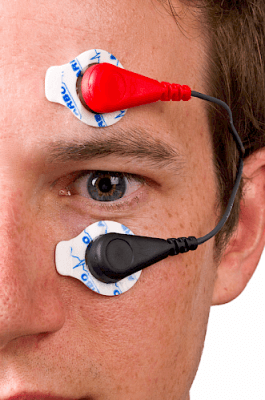
\includegraphics[width=0.51\textwidth]{img/eog.png}
        \caption{An~electro-oculography device.~\cite{fig:eog} }
        \label{fig:eog}
    \end{subfigure}
    \hfill
    \begin{subfigure}[b]{0.45\textwidth}
        \centering
        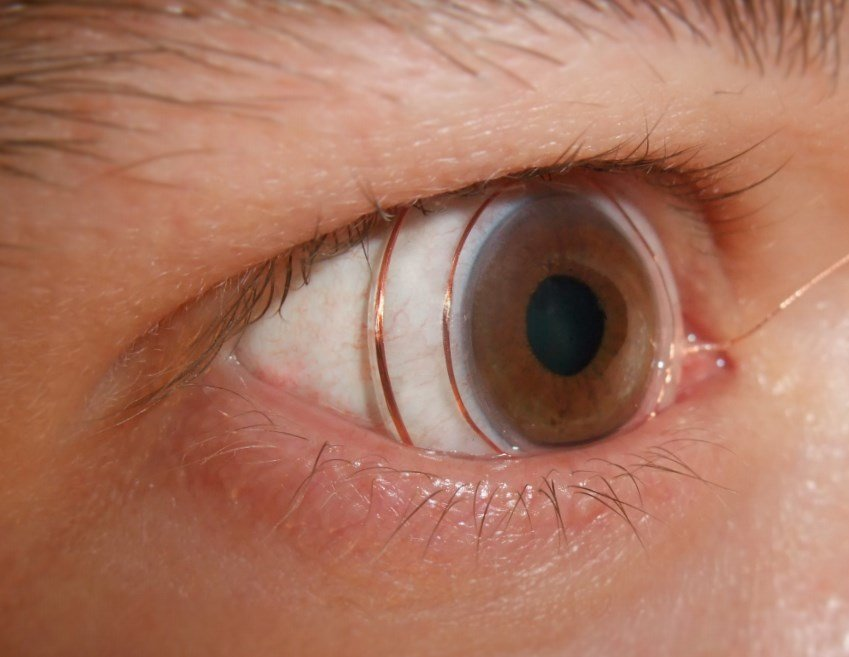
\includegraphics[width=\textwidth]{img/scleral-contact-lens.png}
        \caption{A~scleral contact lens with wire coil.~\cite{fig:scleral-lens}}
        \label{fig:contact-lens}
    \end{subfigure}
    \caption{Examples of intrusive eye tracking devices.}
\end{figure}

\begin{figure}[!ht]\centering
    \includesvg[width=0.60\textwidth]{img/basic-vod}
    \caption[Typical video-oculography setup using  method of corneal reflection.]{Typical video-oculography setup using method of corneal reflection.~\cite[p.~16497]{anuradha2017review}.}
    \label{fig:basic-vod}
\end{figure}

\subsection{Video-based methods}
\emph{Photo} and \emph{video-oculography} group together methods that record eye images with the~use of cameras or video cameras to measure eye movements. The~recording device is either attached to the~users head; head-mounted; or placed near the~user; table-mounted. Devices that are used in the~these methods are non-intrusive, even if the~device is mounted on the~head, because the~actual measurement is not made by direct physical contact with the~user.

Hansen has described video-based methods and their general process in great detail. The~publication is, despite its age, still relevant today because the~methods presented have not changed.~\cite{hansen2010}

The~idea behind video-based eye movement measurements is to~inspect distinguishable eye features from captured eye images, which must differ enough to~clearly distinguish between eye and head movements. These are the~appearance and shape of the~pupil, iris, and cornea.

%The~principles used by these features are further described in Sections \ref{sec:eye-detection} and \ref{sec:gaze-estimation}.
The~techniques that use these features are implemented using computer vision. It is possible to process them manually frame-by-frame. Doing so becomes more time-consuming, inefficient, and unreliable with each added frame. Multiple errors can be made during the~process.

The~most widely applied method for measuring eye movements is the~one based on corneal reflexion, example shown in Figure \ref{fig:basic-vod}, which involves the~use of -- at least -- one camera and a~near infrared (NIR) light source to~produce glints on the~eye cornea. The~relative position of the~glint and the~pupil centre is measured to estimate \emph{gaze direction}. Infrared (IR) light is used because it is invisible to the~naked eye and cameras can capture it. This property is useful for controlling the~lightning conditions in the~environment. It is more suited for indoor setups, where natural light can be controlled and IR rays can bounce around.
The~natural light can be also utilised for the~same purpose, but it offers a~poorer contrast~\cite{hansen2010}.

It is impossible to make an~absolutely precise gaze estimate; always a~certain deviation from the~real line of sight must be taken into account, as shown in Figure \ref{fig:basic-vod}. P represents the~pupil on the~human eye ball and G is the~glint created by the~light source. The~camera image plane is the~captured eye image, in which P and G indicate the~position of the~pupil and the~glint.~\cite{anuradha2017review}

\subsubsection*{ET process}
Each \emph{video-oculography} system must go through the~same process, shown in Figure \ref{fig:ET-process}, to~estimate \emph{gaze direction}. In the~initial step, this procedure requires image data. At least one camera is needed. The~image is processed to~determine the~existence of the~eye and to~detect its position, which can be used directly by an~application or further used to~estimate \emph{gaze direction} -- PoR, which is the~final output an~application can receive from the~system. For this to happen, the~position and rotation of the~head needs to~be tracked.

\begin{figure}[!ht]\centering{}
    \includesvg[width=0.8\textwidth]{img/ET-technique}
    \caption[Components of eye tracking process.]{Components of eye tracking process.~\cite{fig:vbprocesscomponents}}
    \label{fig:ET-process}
\end{figure}

\subsubsection*{Tracking head position}
One possible solution is to~simply sacrifice a~degree of freedom and fix the~head in one place in~space -- resting a~chin on a~raised support. It~is functional but not optimal, because there are techniques that solve this. Another device or system dedicated to~tracking the~head position needs to~be used in parallel.
If the~system is table-mounted, the~head position is already handled by some \emph{gaze estimation} algorithms. %; more about this in Section~\ref{sec:gaze-estimation}.
Meanwhile, this is impossible for head-mounted systems, because they move simultaneously with the~head, so the~\emph{gaze direction} behaves the~same. Another device or system dedicated to~tracking the~head position needs to~be used in parallel.

There are several positional tracking systems. Some track the~absolute position of the~user in a~room, such as~VICON tracker, Lighthouse from Valve, ART trackers, OptiTrack, \ldots

Other systems can detect the~position of the~head while being head-mounted. This is a~simultaneous localisation and mapping (SLAM) problem, which is solved, for example, by the Intel T265 tracking camera. However, this is beyond the~scope of this thesis.

Table-mounted devices estimate PoR on a~surface of interest -- usually a~monitor or a~TV screen -- which might be too restrictive because they cannot move with the~user and may experience difficulties registering eye positions from angles invisible to the~camera. Wearable eye gaze tracking devices use virtual scene cameras to~measure gaze in 3D space.~\cite{cognolato2018}

\section{Eye detection}
\label{sec:eye-detection}

This section derives information mainly from Hansen~\cite{hansen2010}. The~purpose of \emph{eye detection} is to~determine the~existence of the~eye and its position from the~captured eye images. It is crucial, in order to successfully perform it, to find an~eye model that is flexible enough to account for changes in the~eye's appearance without being computationally too expensive. Techniques use computer vision algorithms to analyse captured eye images to obtain information that describe the~eye's status, appearance, lighting conditions, and reflectivity. Specifically, the~viewing angle, head position, occlusion by the~eyelid, degree of eye openness, and position and colour of the~iris. These are very specific features that drastically change the~appearance of the~eye.
Eye models are determined by approaches that use the~shape or appearance of the~eye. 
%There are also hybrid ones that use both approaches and benefit from their respective advantages. 

\subsection{Shape}

These approaches create eye models using shapes of eye features. Their important characteristic is the~ability to handle changes in the~shape, scale, and rotation of the~eye. Models are defined by a~geometric shape that is either rigid or deformable, based on its parameters. 

\subsubsection*{Rigid shape}
\emph{Simple elliptical shape} is an~computationally efficient rigid model that takes advantage of the~eye features that look elliptical; iris and pupil. The~current state of those features under different viewing angles is found by edge detection algorithms. The~iris is detected by finding the~limbus, which is the~boundary between the~iris and the~sclera, and the~pupil by detecting its edge with the~iris. The~variability of these features is restricted to two degrees of freedom that describe eye movements; pan and~tilt. Higher-contrast images are preferred for easier and more precise edge detection.

\subsubsection*{Complex shape}
More detailed eye models can be made for greater precision. Methods based on a~deformable eye model use for the~eye description generic deformable template, which is modifiable with parameters. One method is used to represent the~eyelids and the~iris. The~former is described by two parabolas with 11 parameters, while the~iris is a~simple circle. Another method describes the~deformable eye with two semiellipses that are defined by six parameters. 

Methods based on a~deformable eye model offer an~accurate and generic representation of the~eye, but they are computationally very demanding and require high contrast images that are taken from a~close distance to the~eye for their proper operation. Algorithms solving these issues incorporate energy minimisation processes of computer vision. The~same approaches are applicable to face recognition. 

\subsection{Appearance}

Appearance-based approaches detect and track eyes directly from captured images, as opposed to shape approaches. The~eye and its features are described by the~colour distribution in the~image or by the~results of \emph{image filters}. The~computer vision techniques employed do not require any knowledge about the~eye itself. These are actually able to model absolutely anything. The~requirement to train a~model is to use a~sufficiently large set of images that represent the~appearance of the~desired object. 
%when the~model is trained on a~sufficiently large dataset of images representing the~appearance of the~desired object.

Methods based on these approaches can have problems with rotation, scale, and detection of the~eye. The~reason for this may be the~insufficient amount and diversity of training data that do not reflect different types of eyes, head orientations, or lighting conditions. 

Information about the~appearance of the~eye is extracted from captured images either directly or by their transformation, which can enhance the~features of the~eye or suppress differences in illumination.

\pagebreak{}
\subsubsection*{Image filtering}
\emph{Image filtering} are techniques used to~modify raster images, either over the~entire image or just in a~selected area. Filtering can be done in two ways, either by filtering only one pixel value or by adjusting a~pixel, based on its near surrounding neighbours. These techniques include, for example, brightness and contrast adjustments, gamma correction, thresholding, blurring, edge detection, and convolution.~\cite{trnka2020thesis}

\subsubsection*{Eye features}
Captured eye data can be transformed by filters. Filter responses to a~given image can also be used for individual eye features. Some are more appropriate than others. Limbus boundary detection is easily implementable but offers low precision~\cite{cognolato2018}. Generally, explicit eye edge detection may not always be correctly detected due to changes in light, image focus, occlusion, or eyelid cover.

Eye images taken from a~reasonably close distance allow the~pupil to be a~reliable feature. It depends on the~pupil, and the~iris appears darker than in other areas. This might require higher-contrast images. One method uses an~iterative threshold algorithm that searches for two dark regions. However, this method alone is insufficient in some cases. It could confuse the~pupil with areas with dark shadows, eyebrows, or even areas of individuals with darker skin. There is an~improvement for this method that uses an~NIR light source.

\subsection{Dark and Bright pupil}
\label{sec:dp-method}

These are two methods that extend the~eye detection method by localisation of the~pupil with an~IR light ray. It is used to increase the~pupil contrast in captured images for more robust eye detection.

The~methods depend on the~angle of light entering the~pupil. When the~IR light bounces back from the~eye to the~camera, the~pupil brightens up. On the~contrary, when the~light is at an~angle away from the~camera, it creates an~effect where the~pupil appears much darker. 

This Czech thesis presents an~implementation of the~dark pupil method using a~\emph{convolutional neural network} (CNN)~\cite{trnka2020thesis}.

\subsection{Purkinje images}
Another characteristic of the~eye that is observed is the~behaviour of how light reflects off its surface. These features were found by Jan Evangelista Purkyně. They are named after him and called \emph{Purkinje images}. In the~context of ET, IR light is used to produce different types of reflexions on the~eye, which are then detected by algorithms.

Exactly four distinct \emph{Purkinje images} can be recognised. First one (P1) is reffered to as a~glint, which is reflexion of the~outer side of the~cornea. Second (P2) is the~reflexion from the~back side of the~cornea. Third (P3) bounces off the~front side of the~eye lens. Fourth (P4) image captures the~reflectivity of the~back side of the~eye lens.~\cite{ugwitz2020thesis}

\pagebreak{}

\section{Gaze estimation}
\label{sec:gaze-estimation}
Determining gaze is to be understood as the~gaze direction or PoR, which is a~2D coordinate on a~surface. \emph{Pupil Centre Cornea Reflexion} (PCCR) is a~method that uses an~NIR light source to produce the~first Purkinje images while simultaneously darkening the~pupil using the~dark pupil method. This results in a~very contrasting image of a~glint and a~pupil. These features are easy to detect, so their positions are determined. It is the~most widely used ET method to date~\cite{tobii-eye-trackers}. Gaze is estimated by their relative position, which is used by two different methods.~\cite{cognolato2018}

However, the~position and orientation of the~head need to be taken into account for systems that do not operate with a~fixed head. In these cases, the~head movement must be compensated for. This problem is not solved with HMD systems because they move simultaneously with the~head.~\cite{anuradha2017review}

\subsection{2D regression}

2D regression is a~group of methods that use the~position of the~pupil and the~glint of the~eye to map directly to a~PoR. This mapping is expressed by some polynomial function or by a~neural network. There are 2D regression methods that are capable of head compensation during polynomial mapping~\cite{anuradha2017review}. Some are able to address this by adding an~additional camera, which requires stereo calibration~\cite{hansen2010}.

For these methods, it is essential to use a~calibration for the~polynomial function. It is often based on several points on the~screen that are spaced around. The~points cause the~eye to look in a~certain direction. The~camera records the~eye. From this eye image, the~position of the~pupil, the~glint and their relative vector are determined and assigned to a certain gaze vector or PoR on the~screen according to a~specific calibration point. This operation finds the~correct parameters for the~polynomial function from them. The~accuracy of gaze estimation is improved with a~larger number of calibration points.~\cite{anuradha2017review}

\subsection{3D model}
Then there are methods that create a~geometric 3D model of the~eye from the~detected features, and the~estimated gaze originates from the~centre of the~cornea as the~optical axis of this 3D model. These methods utilise the~similarity of the~shape and size of the~eyes.~\cite{anuradha2017review} 

For the~complete construction of the~model, knowledge of the~camera position and light is required, which can be obtained by calibration. For cases where the~head position keeps changing, the~head position must be constantly evaluated. External positioning systems can be useful for this. The~basic device that uses a~3D model to estimate gaze is one IR camera and one IR LED. Such a~solution might require calibration. However, there are many other solutions that add multiple LEDs and cameras to the~system that might no longer require a~calibration. If it does, only once in a~while. For example, if multiple users are using the~device, each would need their own calibration. As the~number of cameras and LEDs increases, so does the~accuracy and quality of the~measurement, while the~need for calibration decreases.~\cite{trnka2020thesis}

\chapter{Analysis}
\begin{chapterabstract}
This chapter covers the~analysis of current gaze tracking practises, systems implementing ET, the~latest VR devices with ET and the~capabilities of Unreal Engine with possibilities of implementing ET in it.
\end{chapterabstract}

\section{Gaze tracking}

ET technology combined with VR allows one to~estimate the~gaze direction in a~3D world, which is a~3D vector. Various techniques that solve the~manipulation, classification, and storage of this line of sight are part of gaze tracking.

\subsection{Fundamentals}
The~way an~eye moves can be described as a~continuous sequence of two alternating actions;~fixation and saccade.~\cite{hansen2010, anuradha2017review}

\begin{description}
    \item[Fixation] is a~stable but non-static gaze state that rests on a~small area for a~period of time. A~gaze can only be classified as a~fixation if it remains in the~area for a~defined minimum threshold duration -- usually 80~ms.
    \item[Saccade] is a~gaze state that indicates rapid movements of the~eye between fixations. It can be classified as such if the~gaze leaves the~small area prior to fixation classification.
\end{description}


Fixation is the~main metric used in ET, but it requires context. In order to~use gaze to~determine fixation within a~3D scene, it is first necessary to~segment the~scene into several logical sections.


\subsubsection*{Region of Interest}
This segment is called \emph{Region of Interest} (RoI), which provides the~context for the~fixation, i.e., the~gaze target. These can be defined as large areas with multiple objects or, alternatively, as small details. Each virtual scene contains information about its objects and their absolute positions in its coordinates. It is reasonable to~create RoIs according to~individual objects in a~given scene.~\cite{ugwitz2020thesis}

An~ET experiment consists of subtasks during which fixations and saccades at different RoIs are captured over time to~determine when and where the~subject gazed at. This information can be used in the~creation of further structures that provide more context to the~subject's behaviour during an~experiment.~\cite{koenig2019}

\subsubsection*{Scanpath}
One of these is \emph{scanpath}~\cite{anuradha2017review}, which consists of an~alternating sequence of fixations and saccades. These are not only useful for storing the~sequence of eye movements over time, but also can be used to~infer the~duration and distance between two different fixations.

With its combination, more precise information is obtained about each \emph{region of interest}, from which one can infer how much time elapsed before the~first fixation in the~RoI or how many and which regions were visited before. Another related metric is \emph{gaze duration}, which sums the~duration of all fixations in a~single RoI.

\subsection{Gaze data}
\label{sec:gaze-data}
The~data are constructed in real time during the~experiment or after its end. Everything depends on the~deployed hardware. It is recommended to have all available performance ready to~use for the~experiment itself. For later processing of ET data, it is crucial to~record the~gaze data first. Sources used for this section~\cite{ugwitz2020thesis, koenig2019}

\begin{figure}[!ht]\centering
    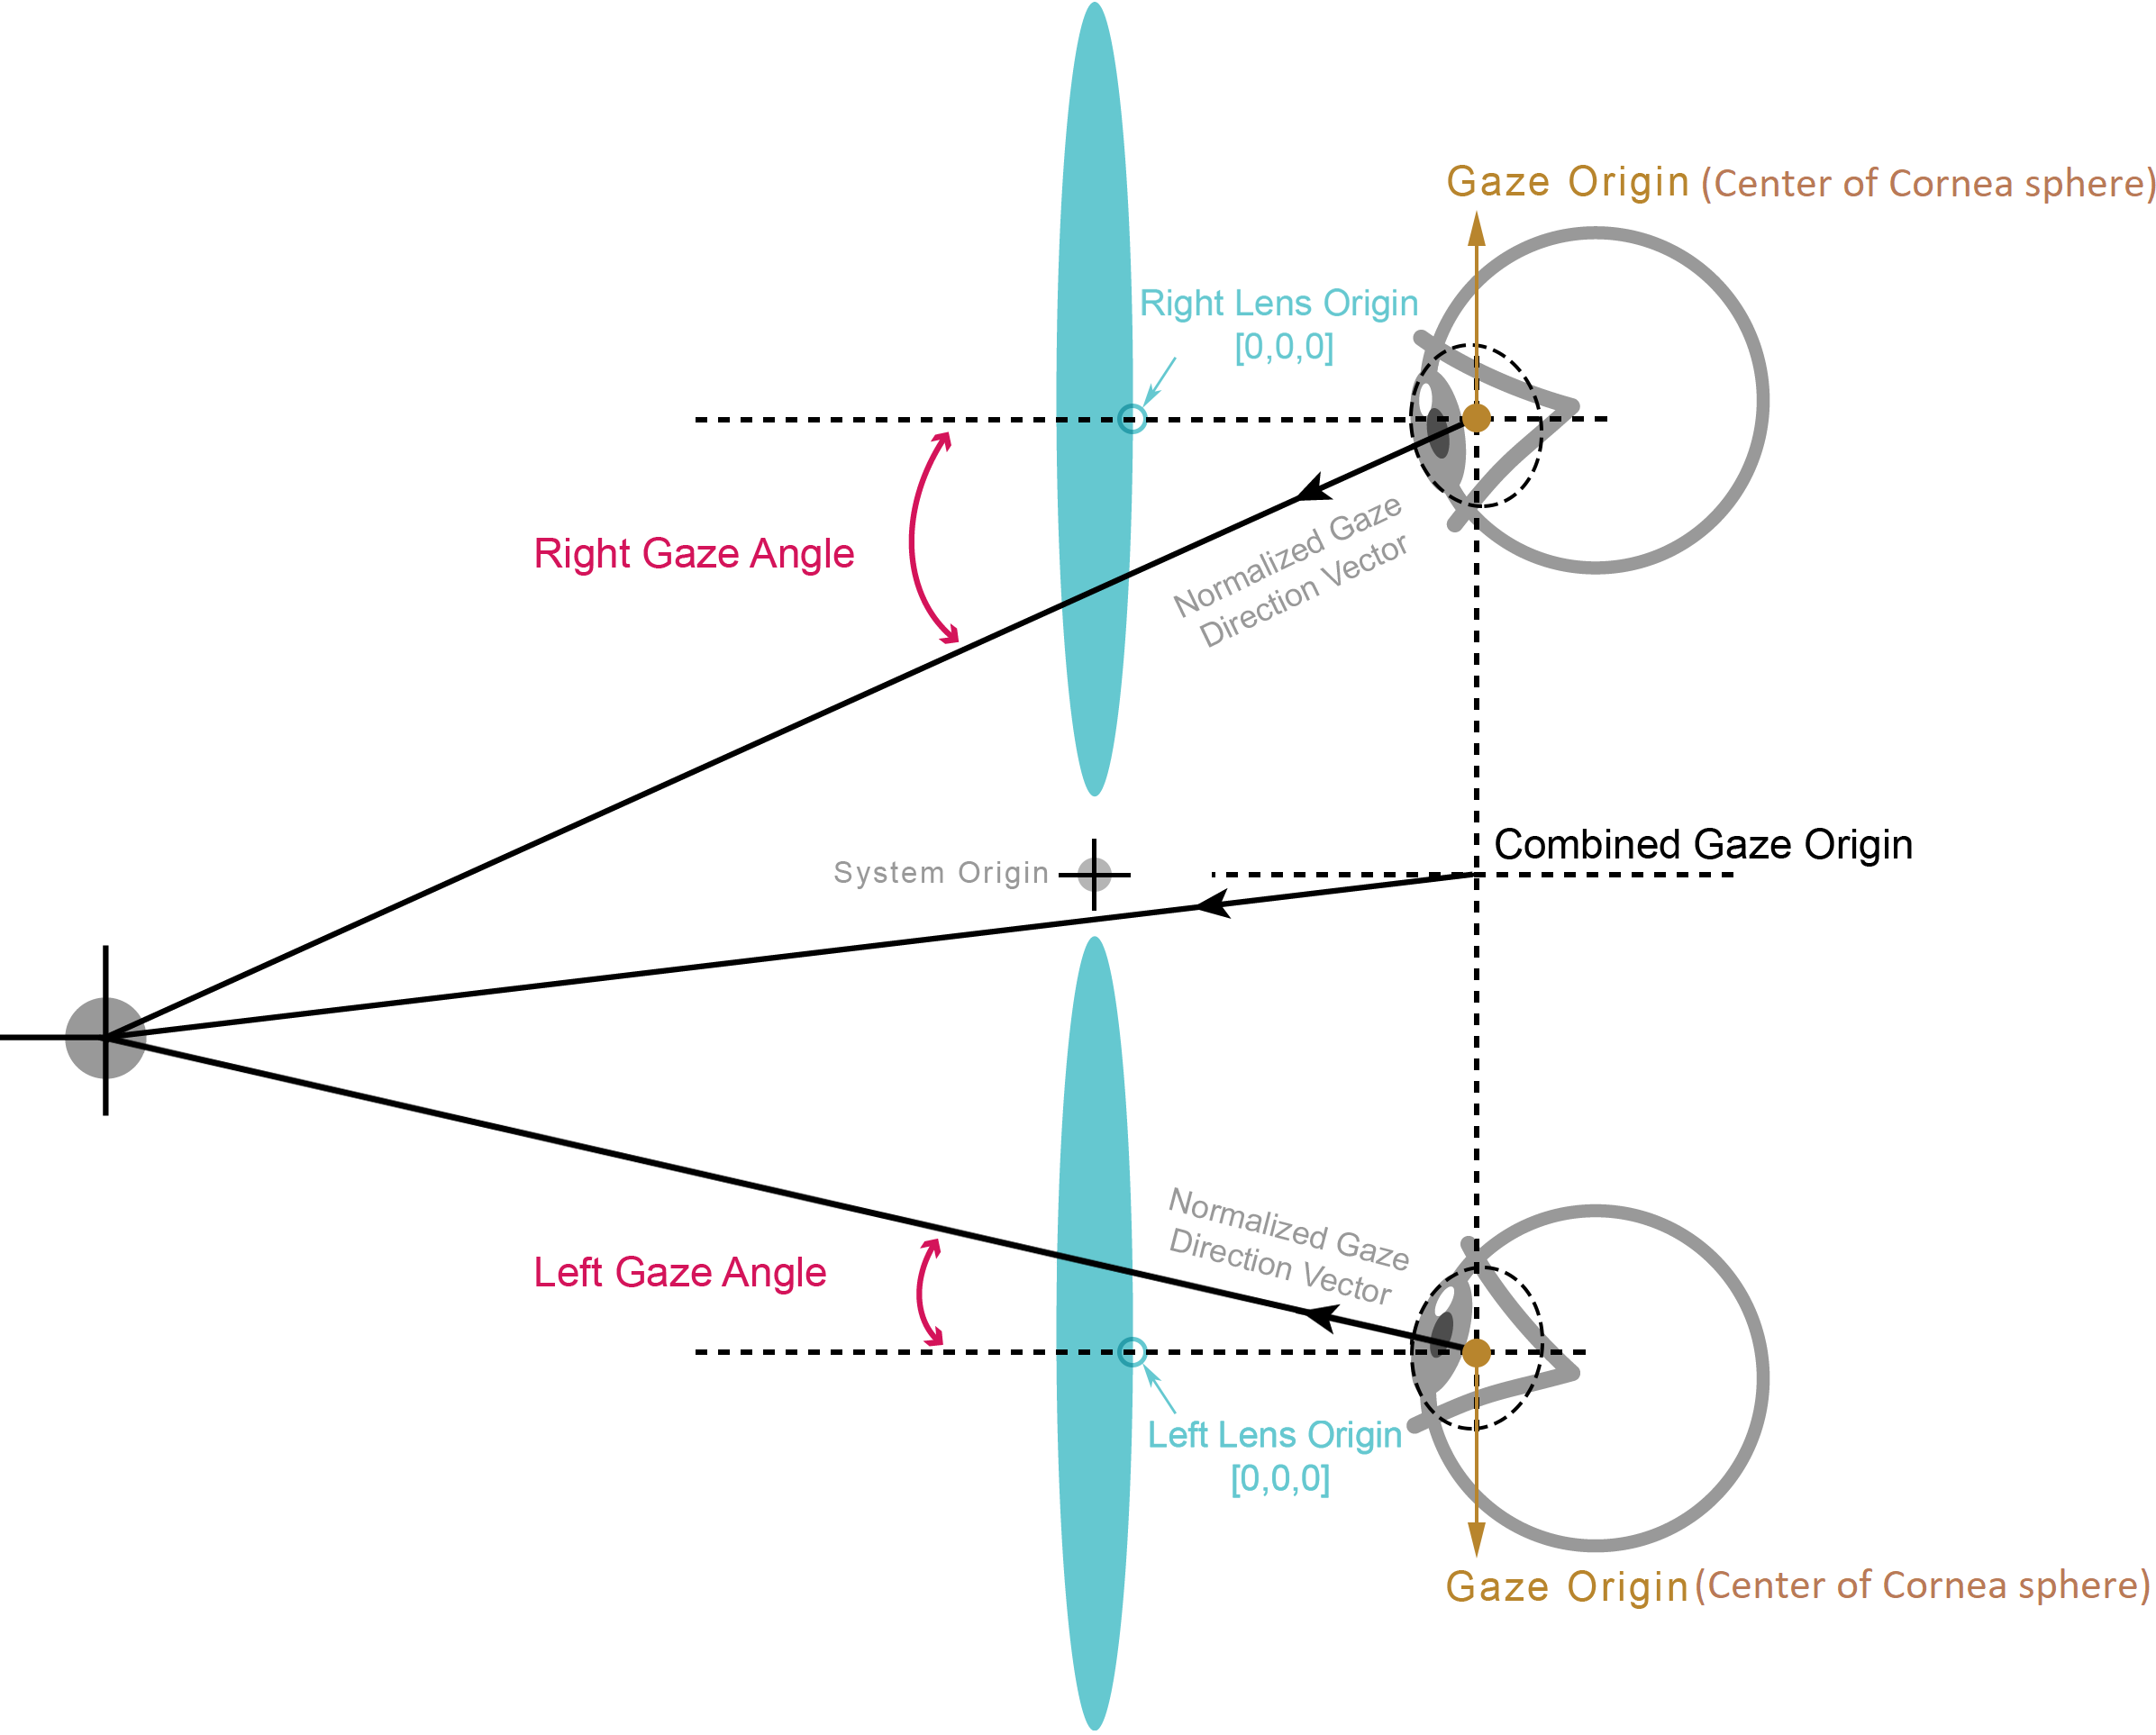
\includegraphics[width=\textwidth]{img/EyeData.png}
    \caption[Detailed scheme of gaze data]{Detailed scheme of gaze data~\cite{sranipal-image}}
    \label{fig:gaze-data}
\end{figure}

\pagebreak{}
\subsubsection*{Gaze structure}

Gaze data are the~result or output of an~ET device, but not every time the~data are suitable for the~use in a~virtual scene. Some eye trackers produce 2D coordinates on a~display surface that represent PoR~\cite{ugwitz2022}. If the~produced data are to~be used in a~virtual scene, it should be a~collection of 3D vectors. This is illustrated in Figure~\ref{fig:gaze-data}. The~gaze itself from a~single eye is represented by two 3D vectors;~normalised \emph{gaze direction} vector and \emph{gaze origin} coordinates.

Both are in a~coordinate system that is related to that particular eye. In this specific situation, the~origin of the~coordinate system is a~fixed point that is not related to the~eye itself because it can account for variations in the~eye positions of different people. Figure~\ref{fig:gaze-data} shows the~use of a~lens in HMD for VR as the~origin of the~eye's coordinate system.

\subsubsection*{Point of Fixation}
Subjects usually have two functioning eyes, so stereo gaze data can be used in their situation. Two separate coordinate systems, eye positions, and gaze directions. In the~best case, the~intersection of these two vectors in world coordinates can be used to~identify \emph{Point of Fixation} (PoF).

However, the~problem is that the~absolute precision of these vectors is not guaranteed due to~limitations in eye detection using video-based ET devices, which return acceptable results only for perfect calibrations. The~farther in a~scene the~eye gazes, the~more precision is required. In this case, the~accuracy must be below $0.5$ degrees.

The~difference between \emph{fixation} and PoF is that fixation describes the~type of gaze, and PoF is the~point in space where fixation occurs.

\subsubsection*{Combined gaze}
An~alternative to~stereo gaze data in multiple implementations of ET in HMDs is a~combined gaze vector. The~combined gaze origin is the~average of the~two origin coordinates, and the~direction of gaze is the~normalised sum of the~two gaze vectors. Each vector calculation is performed in the~ET device coordinate system.

\subsubsection*{Data processing}
To~search for fixations using the~combined gaze in the~scene, one has to~resort to~collisions. Sending a~ray in world coordinates from an~eye into the~scene -- \emph{raycasting}. PoF is the~first object (RoI) hit by the~ray.

The~search for fixations can be done in~real time during the~experiment or sometime after its end. In the~case of offline evaluation, it is first necessary to~gather the~scene information correctly together with the~gaze data during the~experiment. The~essential data consist of time in seconds or milliseconds, a~3D coordinate that reflects the~position of the~scene camera in the~world, its rotation, and the~gaze origin with its direction; two 3D vectors in world coordinates.

These are saved in a~CSV file or in an~internal database. During prototype testing, it is more convenient to~save data in CSV because the~file can be deleted at any time after a~failure, as opposed to~deleting non-valid entries from a~database. Performing offline computations is meaningful only when the~gaze data are processed and visualised in several different ways that clearly consume computational power. If a~search for PoF is performed alone, there is no reason not to~compute it in real time.

\pagebreak{}
\subsection{Visualisations}

Analysing the~existing solutions later in Section~\ref{sec:solutions} found that there are generally two ways to visualise gaze data in a~virtual environment. Many analyses of gaze data consist of recording them in external files and processing or visualising them with a~help of a~statistical programme. The~basis for all visualisations are PoFs in 3D space. These points are then transformed or classified into more specific structures. 

\begin{description}
    \item[Heatmap] is a~graphical representation of data where each value on a~map is represented by a~colour from a~predetermined spectrum. Typically, this is a~transition from blue, representing the~minimum value, through green and yellow to red, which indicates the~maximum value. In the~context of fixations, higher heatmap values are indicative of a~denser concentration of PoFs or their individual strength; the~duration of fixation.
    \item[Gaze trail] is a~visual representation of \emph{scanpath}, where PoFs are displayed by a~simple cube or sphere primitive. Saccades connect these primitives in space with lines.
\end{description}

This interesting study from 2005 explores attention search in a~virtual environment~\cite{kit2014}. This is an~experiment that explores visual search for different objects in a~virtual three-room apartment with the~participation of several subjects over multiple days.
They used a~custom HMD with lower resolution to~collect the~data, given the~age of the~study. Eye images, camera view, and participant's position in the~scene were recorded for an~evaluation. The~whole situation was reconstructed offline for analysis.

The~PoF was obtained using an~algorithm that took the~eye position from an~eye image and used its screen coordinates to~extract a~60x60 pixel square from the~camera scene footage. From these few pixels, it was evaluated which object occupied the~most pixels. The~same object's location was used as the~3D fixation coordinate.

It is possible to~visualise 3D data by condensing them onto a~2D map. They created several graphs and 2D heatmaps from the~gathered PoFs. For example, the~floor plan of an~experiment scene can be overlaid with a~heatmap that describes the~spatial intensity of gaze data.

\begin{figure}[!ht]\centering
    \begin{subfigure}[b]{0.4\textwidth}
        \centering
        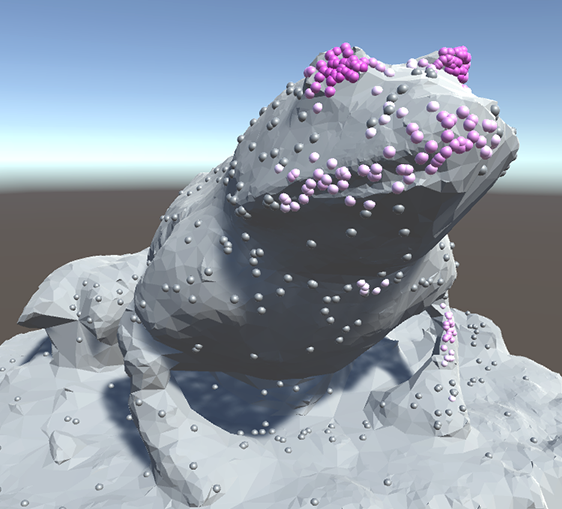
\includegraphics[width=0.9\textwidth]{img/ugwitz-heatmap.png}
        \caption{3D Heatmap points~\cite[p. 52]{ugwitz2020thesis}}
        \label{fig:ugwitz-heatmap}
    \end{subfigure}
    \hfill
    \begin{subfigure}[b]{0.55\textwidth}
        \centering
        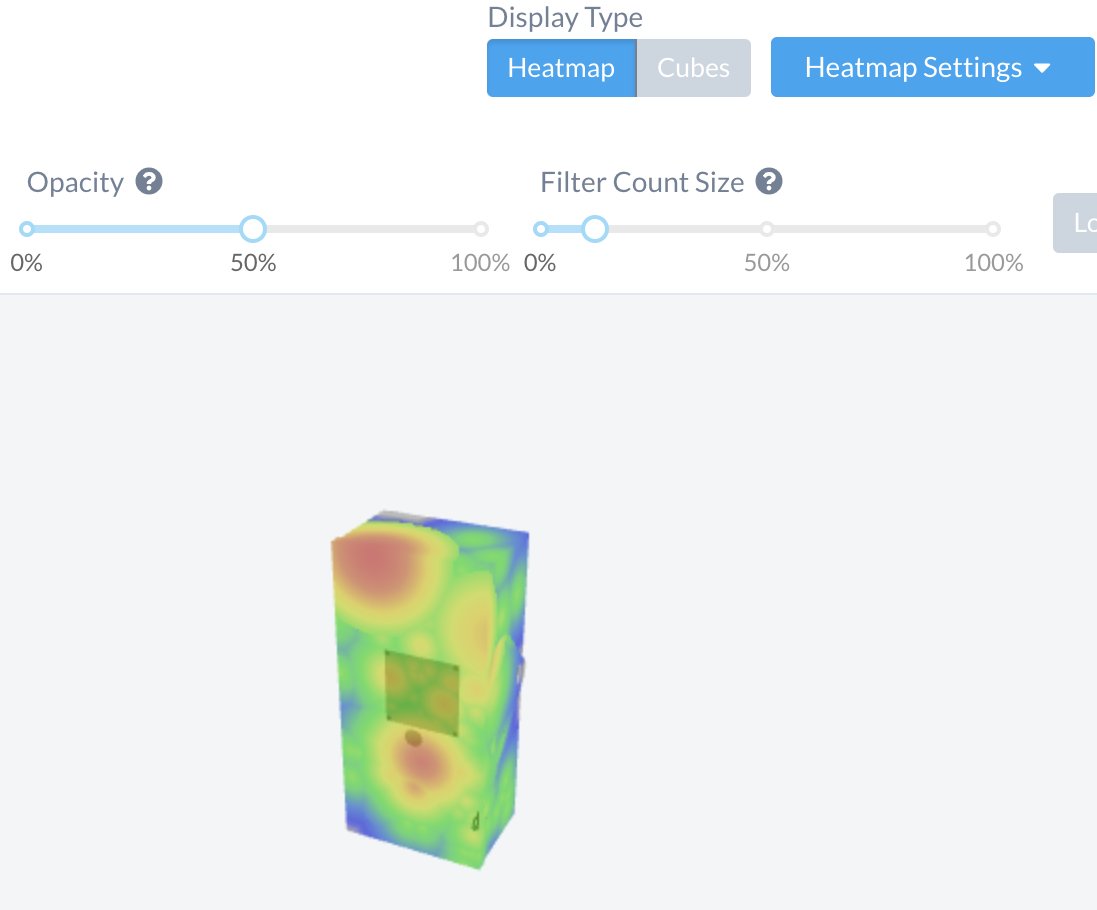
\includegraphics[width=\textwidth]{img/cognitive3d-heatmap.png}
        \caption{Object texture heatmap~\cite{cognitive3d-dynamic-objects}}
        \label{fig:cognitive-heatmap}
    \end{subfigure}
    \caption{Example of two different heatmap approaches.}
\end{figure}

\pagebreak{}
This paper~\cite{ugwitz2022}, which is closely related to a~thesis by the~same author~\cite{ugwitz2020thesis}, visualises heatmaps using 3D points in space that are coloured differently according to the~intensity of a~given fixation, can be seen in Figure~\ref{fig:ugwitz-heatmap}.

Cognitive3D software visualises gaze data using heatmaps and visual trail. Heatmaps are generated in a~different way. They draw it on the~wireframe of a~3D model -- Figure~\ref{fig:cognitive-heatmap} -- assumably onto a~texture. The~algorithm they use to do this is proprietary. For real-time visualisation of gaze data, without the~need to collect and evaluate the~data offline, the~method of drawing heatmaps on objects is more suitable. 


\section{Current hardware}
\label{sec:hardware}

ET devices implemented in VR HMDs are portable devices that have only recently seen their first prototypes. The~same applies to the~first truly usable VR headsets that have started to~appear since Oculus' first attempt with its \emph{Rift DK-1} headset. This was immediately followed by the~\emph{DK-2} version. HTC joined in on~this with their VIVE headset. They were all released in a~short period of time before 2016, which is exactly the~year when all the~aforementioned were extended with an~SMI eye tracker.~\cite{ugwitz2022}

Unfortunately, SMI announced that it discontinued the~production and support of its ET devices when it was acquired by Apple in 2017~\cite{iMotions-endSMI}. Regardless of this whole situation, Tobii created an~ET Development Kit for HTC VIVE that was not bundled with the~heatset itself. It had to be purchased separately and mounted inside a~very confined space around the~lenses~\cite{tobii-oldHTC}. Modern headsets are made with ET integrated into them by design. Manufacturers have two options. They either develop ET devices themselves as their proprietary solution or leave it to a~third-party. One of them is Tobii, which dominates the~ET market.~\cite{ugwitz2020thesis}

\subsection{Tobii}
This company is exclusively specialised in eye tracking. Since their inception, when they released the~world's first plug-and-play ET device in 2002~\cite{tobii-history}, they have grown to~become a~global leader in the~industry.

\subsubsection*{Design}
Current Tobii eye tracking systems are based on non-intrusive video-based tracking that uses the~PCCR method. Their implementation uses multiple NIR light sources to~create reflexion patterns, several glints, on the~cornea and pupil, which are recorded by cameras. They use an~advanced image processing algorithm based on a~physiological 3D eye model to~detect the~eye and estimate the~gaze.~\cite{tobii-eye-trackers}

Most of their devices use the~dark and bright pupil method for eye detection, except for wearable devices that use only the~dark pupil method. All~of their devices use the~method mentioned using a~3D eye model for gaze estimation.~\cite{tobii-dark-pupil}

\subsubsection*{Wearable device}
An~example of their wearable eye trackers is Tobii Glasses 3, shown in Figure~\ref{fig:tobii-glasses3}. The~device is designed to~handle real-world ET research. A~robust system is in place, consisting of eight NIR illuminators for each eye separately that create glints. The~single eye with glints is then captured by two very small cameras with a~sampling rate of 100 Hz. A~one-point calibration is performed before measurement. The~device is also equipped with a~full HD camera, which is located in the~beam of glasses. It is a~portable device that does not require a~connection to a~PC, as the~product includes a~recording unit that captures video from the~camera and simultaneously collects ET data to an~SD card. The~accuracy of the~measured data is around $0.6^{\circ}$. The~data are processed and visualised using their analytics software, Tobii Pro Lab. Their Tobii Pro Glasses 3 API allows for a~custom implementation.~\cite{tobii-glasses3}

\begin{figure}\centering
    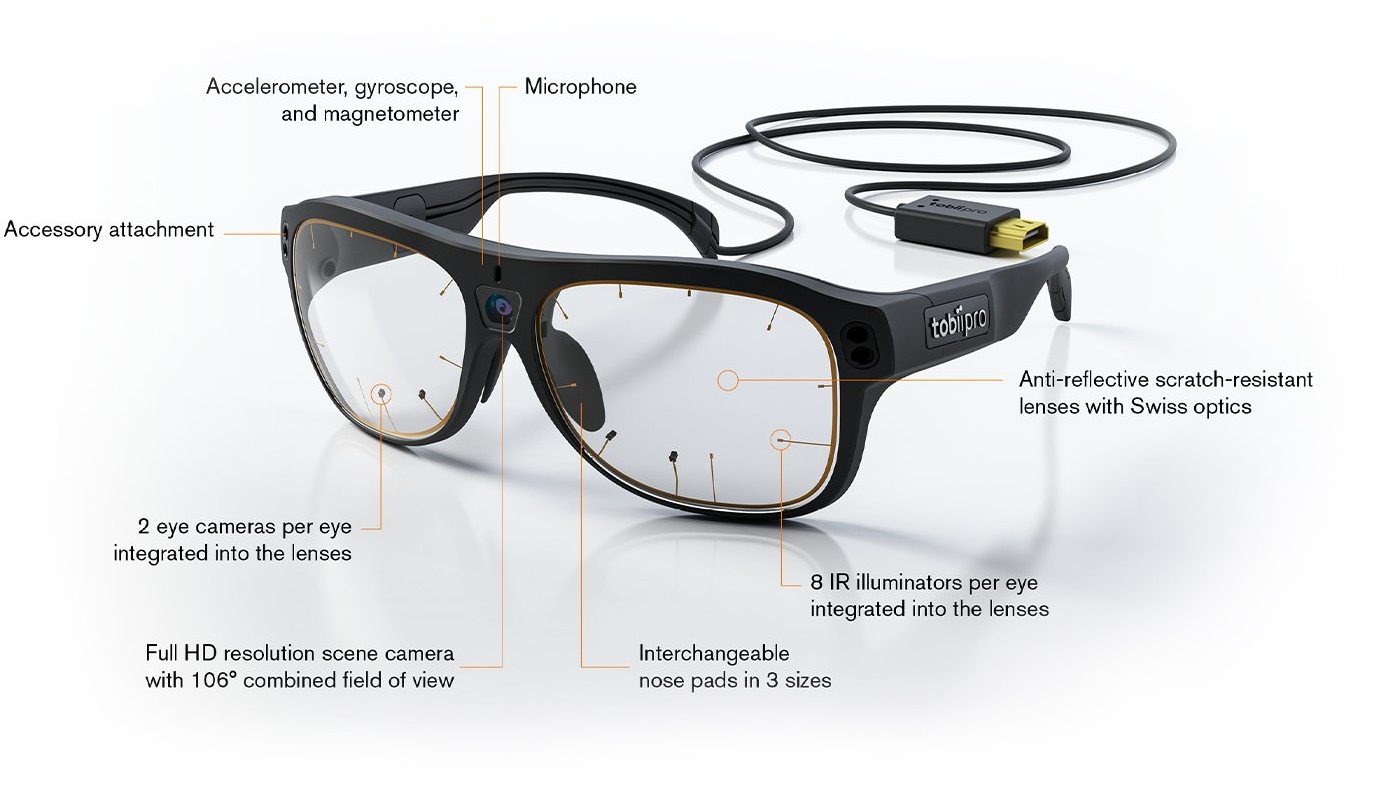
\includegraphics[width=0.9\textwidth]{img/TobiiGlasses3.jpg}
    \caption[Description of Tobii Glasses 3.]{Description of Tobii Glasses~3.~\cite{tobii-glasses3-image}}
    \label{fig:tobii-glasses3}
\end{figure}

\subsubsection*{Table-mounted device}
Tobii also develops table-mounted devices, one of which is the~Tobii Pro Fusion. It is an~ET device that consists of two cameras with a~sampling rate of 250 Hz. The~dual camera setup is used for better head movement tolerance. The~accuracy of this device is $0.3^{\circ}$. Gaze data can be collected and used in their proprietary Tobii Pro Lab software or with the~Tobii Pro SDK, that allows for integration in C, Python programming language,.NET framework or \emph{Unity} game engine.~\cite{tobii-fusion, tobii-pro-sdk}

\begin{figure}[!b]\centering
    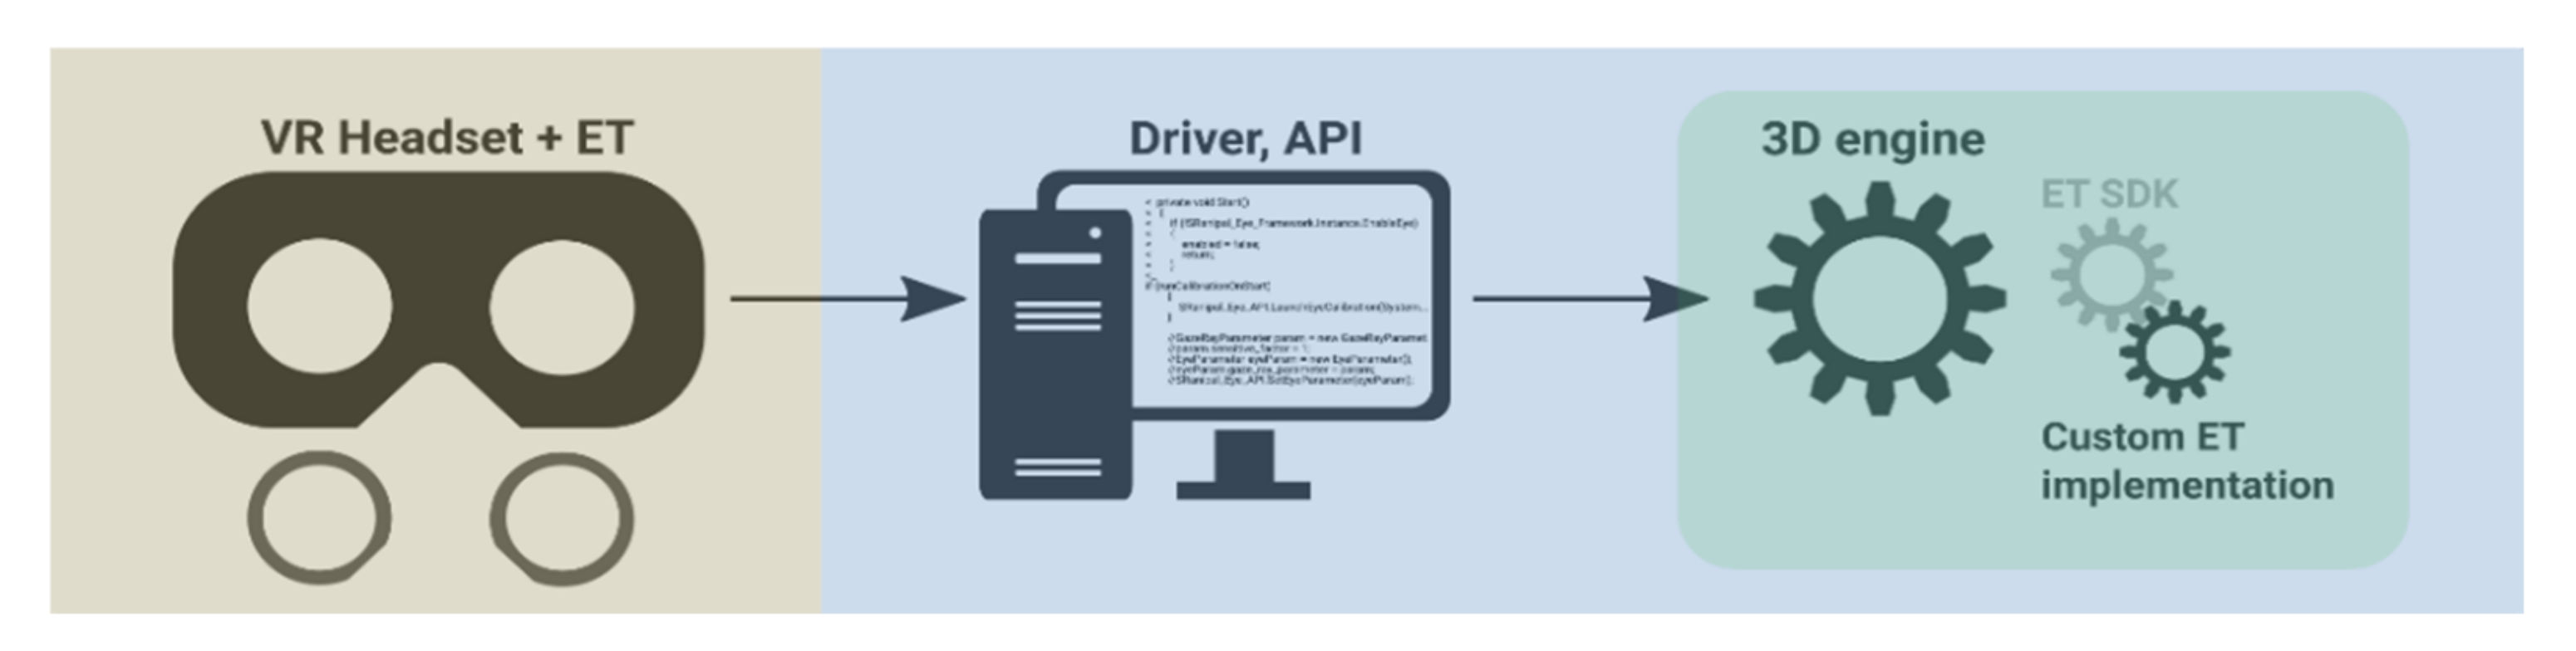
\includegraphics[width=\textwidth]{img/ET-SDK.jpg}
    \caption[Interconnection of ET hardware with SDK.]{Interconnection of ET hardware with SDK.~\cite[p.~4]{ugwitz2022}}
    \label{fig:et-sdk}
\end{figure}

\newpage

\subsection{Integrations in VR HMDs}
\label{sec:integrations}

In~addition to Tobii's own eye trackers, the~company has partnered with various VR headset manufacturers to~provide integration of their ET units. These are HTC, PICO, and HP. Specifically, the~headsets with integrated ET from Tobii include HTC VIVE Pro Eye, HP Reverb G2 Omnicept Edition, PICO Neo 2 Eye and Neo 3 Pro Eye. A~comparison of these devices can be found in Table~\ref{tab:headset-tech-tobii}, which shows their specifications. Frequency of the~output gaze data, measurement accuracy, calibration method, trackable \emph{field of view} (FOV), available \emph{Software Development Kit} (SDK), type of output gaze data, the~state of OpenXR standard implementation, and SDK support for the~two major game engines.

\renewcommand{\arraystretch}{1.15}
\begin{table}[!ht]
\centering
\begin{tabular}{|l||c|c|c|}
\hline
\multicolumn{1}{|c||}{} &
  \begin{tabular}[c]{@{}c@{}}HTC VIVE\\ Pro Eye \cite{tobii-htc-vive}\end{tabular} &
  \begin{tabular}[c]{@{}c@{}}HP Reverb G2\\ Omnicept Edition \cite{tobii-hp-omnicept}\end{tabular} &
  \begin{tabular}[c]{@{}c@{}}PICO Neo 3\\ Pro Eye \cite{tobii-pico3}\end{tabular} \\ \hline\hline
Frequency     & 120 Hz       & 120 Hz          & 60/90 Hz          \\ \hline
Accuracy      & $0.5^{\circ}$--$1.1^{\circ}$    & $<1.0^{\circ}$  & $<1.0^{\circ}$ \\ \hline
Calibration   & 5-point      & 9-point         & 5-point        \\ \hline
Trackable FOV & $110^{\circ}$ & $114^{\circ}$  & $101^{\circ}$  \\ \hline
SDK           & HTC SRanipal & HP Omnicept SDK & Pico SDK       \\ \hline
Stereo gaze    & Yes & Yes    & No     \\ \hline
Combined gaze    & Yes & Yes    & Yes     \\ \hline
%OpenXR Ready  & Yes           & Yes             & Yes            \\ \hline
OpenXR  & Yes           & Yes             & Ready            \\ \hline
Unreal, Unity & Both & Both & Both \\ \hline
\end{tabular}
\caption{Specification of the~latest VR headsets with Tobii ET integration.}
\label{tab:headset-tech-tobii}
\end{table}

\subsubsection*{Software Development Kit}
HMDs communicate with software using a~driver. SDKs are used to add the~communication functionality to the~software. This set of development tools is provided by the~hardware manufacturer. In the~case of VR implementations, the~SDK is in the~form of an~\emph{Application Programming Interface} (API) that returns the~requested data to the~application from some VR runtime that is part of the~hardware driver. As~Figure~\ref{fig:et-sdk} illustrates. 

\subsubsection*{Tobii SDK}
One SDK is available for all HMDs with a~Tobii eye tracker; Tobii XR SDK. The~strength of using this is the~unified access to the~data across all devices. On the~other hand, it offers a~stable release only for the~\emph{Unity} game engine. \emph{Unreal Engine} SDK is still in beta version\footnote{does not work with HTC VIVE Pro Eye} and support for native~C development is only in Alpha. In contrast to~all the~dedicated device SDKs listed in Table 2.1, which offer full support for the~mentioned game engines and native~C.~\cite{tobii-xrsdk} 

\pagebreak{}

\subsection{OpenXR standard}
Until recently, for an~application to be able to use a~specific VR device, a~proprietary API was required to communicate with its hardware driver. Support for different devices in one app required custom driver integration. However, the~Khronos Group has proposed a~new standard to fight this fragmentation; \emph{OpenXR}, which provides high performance cross-platform access to~\emph{Augmented Reality} (AR), \emph{Mixed Reality} (XR) and \emph{Virtual Reality} devices and platforms. 

This includes not only HMDs, but also VR controllers, hand tracking, and eye tracking. New applications are now able to~share the~same interface to~communicate with several different VR, XR, or AR devices, as the~schema on Figure~\ref{fig:openxr-schema} shows. OpenXR is not a~library or an~implemented runtime, but a~specification of how that runtime should look. The~implementation is done by XR device manufacturers themselves.~\cite{openxr-overview, openxr-presentation}

\begin{figure}[!ht]\centering
    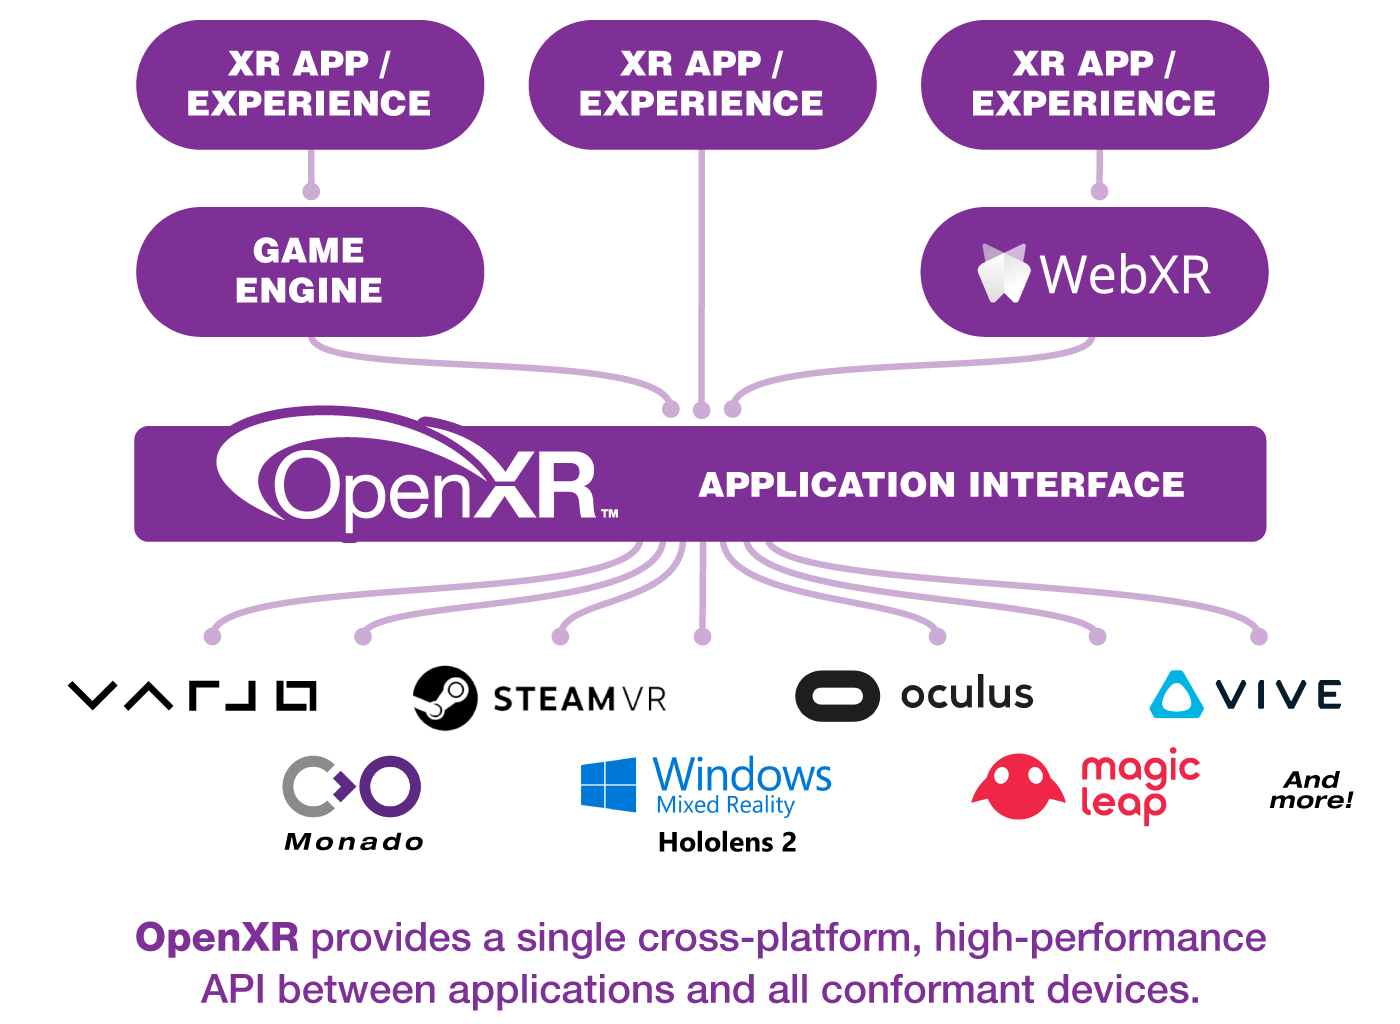
\includegraphics[width=0.75\textwidth]{img/openXR.png}
    \caption[Schema of OpenXR cross-platform access to different XR devices.]{Schema of OpenXR cross-platform access to different XR devices.~\cite{openxr-access-image}}
    \label{fig:openxr-schema}
\end{figure}

An~important aspect of OpenXR is that it uses a~Cartesian right-handed coordinate system to describe the~space in which all vectors are represented; the~$x$ coordinate points to the~right, the~$y$ points up, and the~$z$ coordinate points backward ($-z$ points forward into the~scene).~\cite{openxr-coordinate}

\subsection{Varjo}
\label{sec:varjo}

Varjo is a~Finnish manufacturer of VR and XR HMDs. Their latest VR devices are VR-3 (Figure \ref{fig:varjo-vr3}) and the~Aero headset. All Varjo devices are equipped with Varjo's own proprietary ET solution, not based on Tobii. They claim that their method is ``the~most accurate eye tracking ever integrated into a~VR device''.~\cite{varjo-et}

\subsubsection*{Method}
It is a~method based on 2D regression that is enhanced by the~type of illuminators and camera quality. It uses a~special custom IR illuminator shape that produces complex-shaped glints, instead of dots.

The~robustness of this solution lies in the~ability to~use computer vision algorithms to~distinguish one illuminator from another by examining the~orientation of its glint. Combined with IR cameras that capture eye images at 100~\emph{frames per second} (fps) at a~resolution of 1280x800 pixels, the~accuracy of eye measurement is guaranteed to~be sub-zero degrees even when the~eyes are looking at extreme angles or when glasses are present.

\subsubsection*{Capabilities}
Both headsets are capable of producing combined and stereo gaze output data at 200~Hz. They include an~automatic PID (auto-PID) capability to~adjust the~lens distance and foveated rendering after a~single-point calibration. What~VR-3 has over the~newer and lighter Aero is a~built-in Ultraleap camera for hand tracking, which is visible in Figure~\ref{fig:varjo-vr3}. Headsets use the~native Varjo SDK or OpenXR runtime~\cite{varjo-openxr} to~communicate with apps. Offers support for implementation in native~C and integration into Unreal Engine and Unity game engine.~\cite{varjo-vr3, varjo-aero}

Gaze data output is natively in the~left-handed coordinate system. The~vectors are then represented in a~space where $x$ points to the~right, $y$ points up and $z$ points forward in the~scene; compared to OpenXR, the~z coordinate is flipped. To~start ET, the~device must first be calibrated. This can be done in three different ways. Either a~five-point calibration, which uses statistical data collected from previous calibrations by other users to~enhance the~calibration result, or a~ten-point legacy calibration, which does not include such a~feature. One point cannot be used to~initiate ET, it only serves to~activate foveated rendering.~\cite{varjo-sdk-spec}

\begin{figure}[!t]\centering
    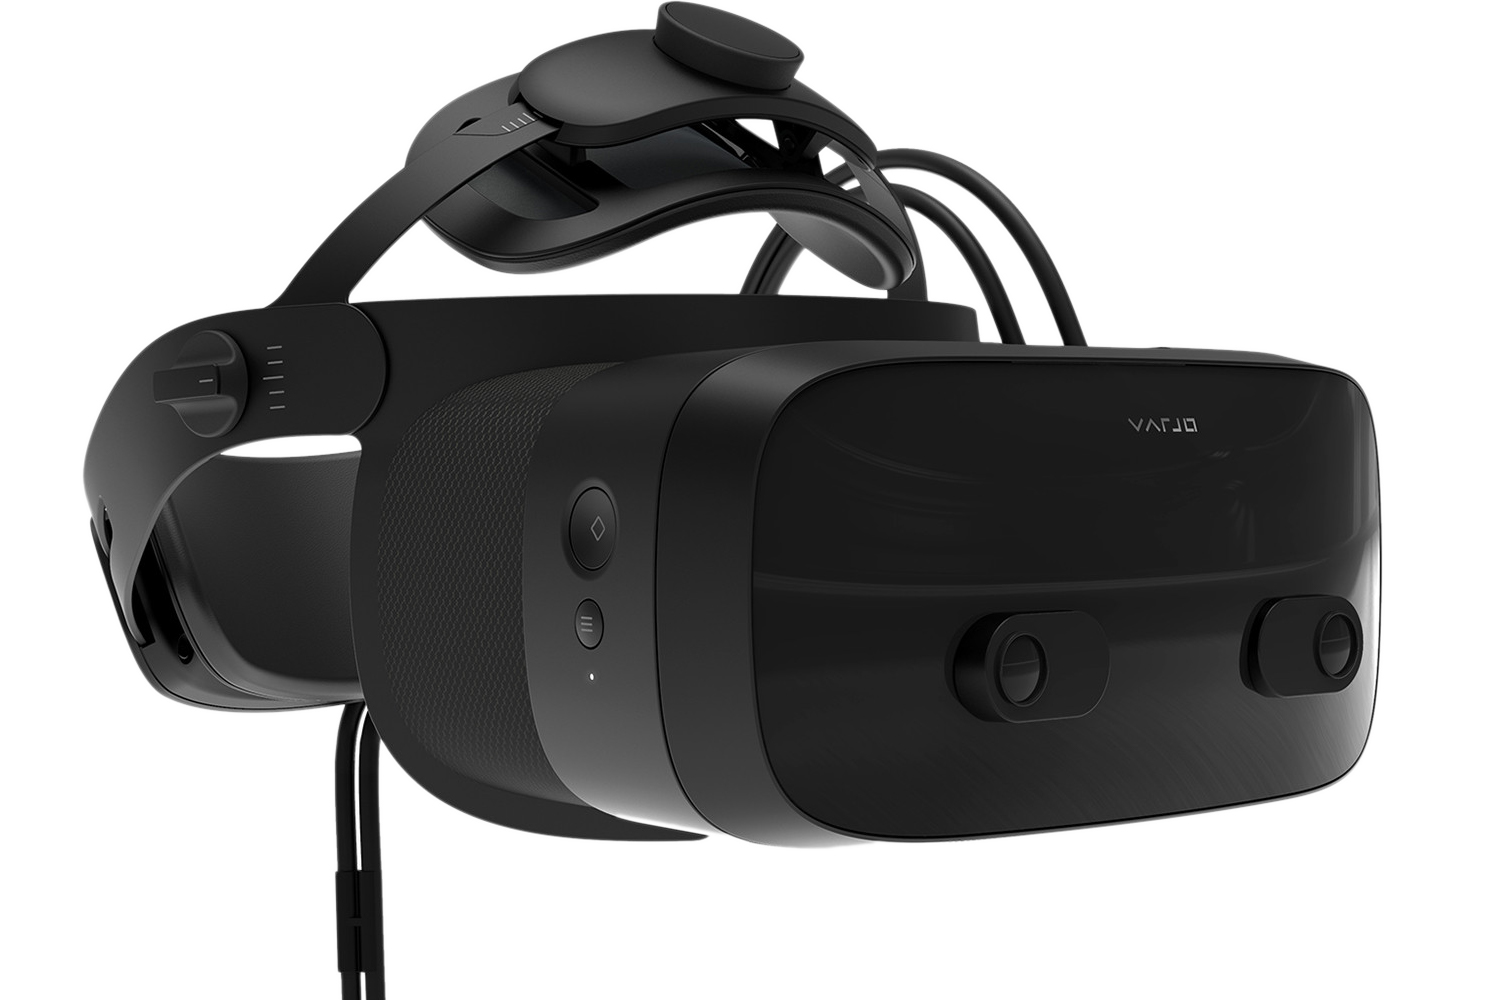
\includegraphics[width=0.7\textwidth]{img/Varjo-VR3.jpg}
    \caption[Varjo VR-3 virtual veality headset.]{Varjo VR-3 virtual reality headset.~\cite{varjo-vr3-image}}
    \label{fig:varjo-vr3}
\end{figure}

Varjo driver has built-in tools to~record gaze data. This feature records them simultaneously with a~video of what the~user has seen. The~output is a~.csv file that can be used to~visualise the~data collected in the~recorded video. The~CSV contains generic gaze data along with their transformation into video coordinates. The~generic data contain the~origin and direction of the~gazes of the~left and right eye and their combined gaze with a~raw timestamp of when the~data were recorded. The~second data in relation to the~video are transformed into 2D coordinates (PoR) and stored together with the~timestamp relative to the~start of the~video.~\cite{varjo-data-logging}


\subsubsection*{Immersive Virtual Reality}
Another Varjo device is the~XR-3 headset for mixed reality, which is almost identical to the~VR-3 but includes the~feature of a~video feed of the~external world. This headset uses two cameras to~record video that can be modified and rendered back on the~internal displays.~\cite{varjo-xr3}

\emph{Immersive Virtual Reality} (IVR) is a~3D projection used in Religious Studies testing Laboratory build by Olomouc Palacký University.~\cite{upol2021procurement}

\begin{figure}[!ht]\centering
    \begin{subfigure}[b]{0.38\textwidth}
        \centering
        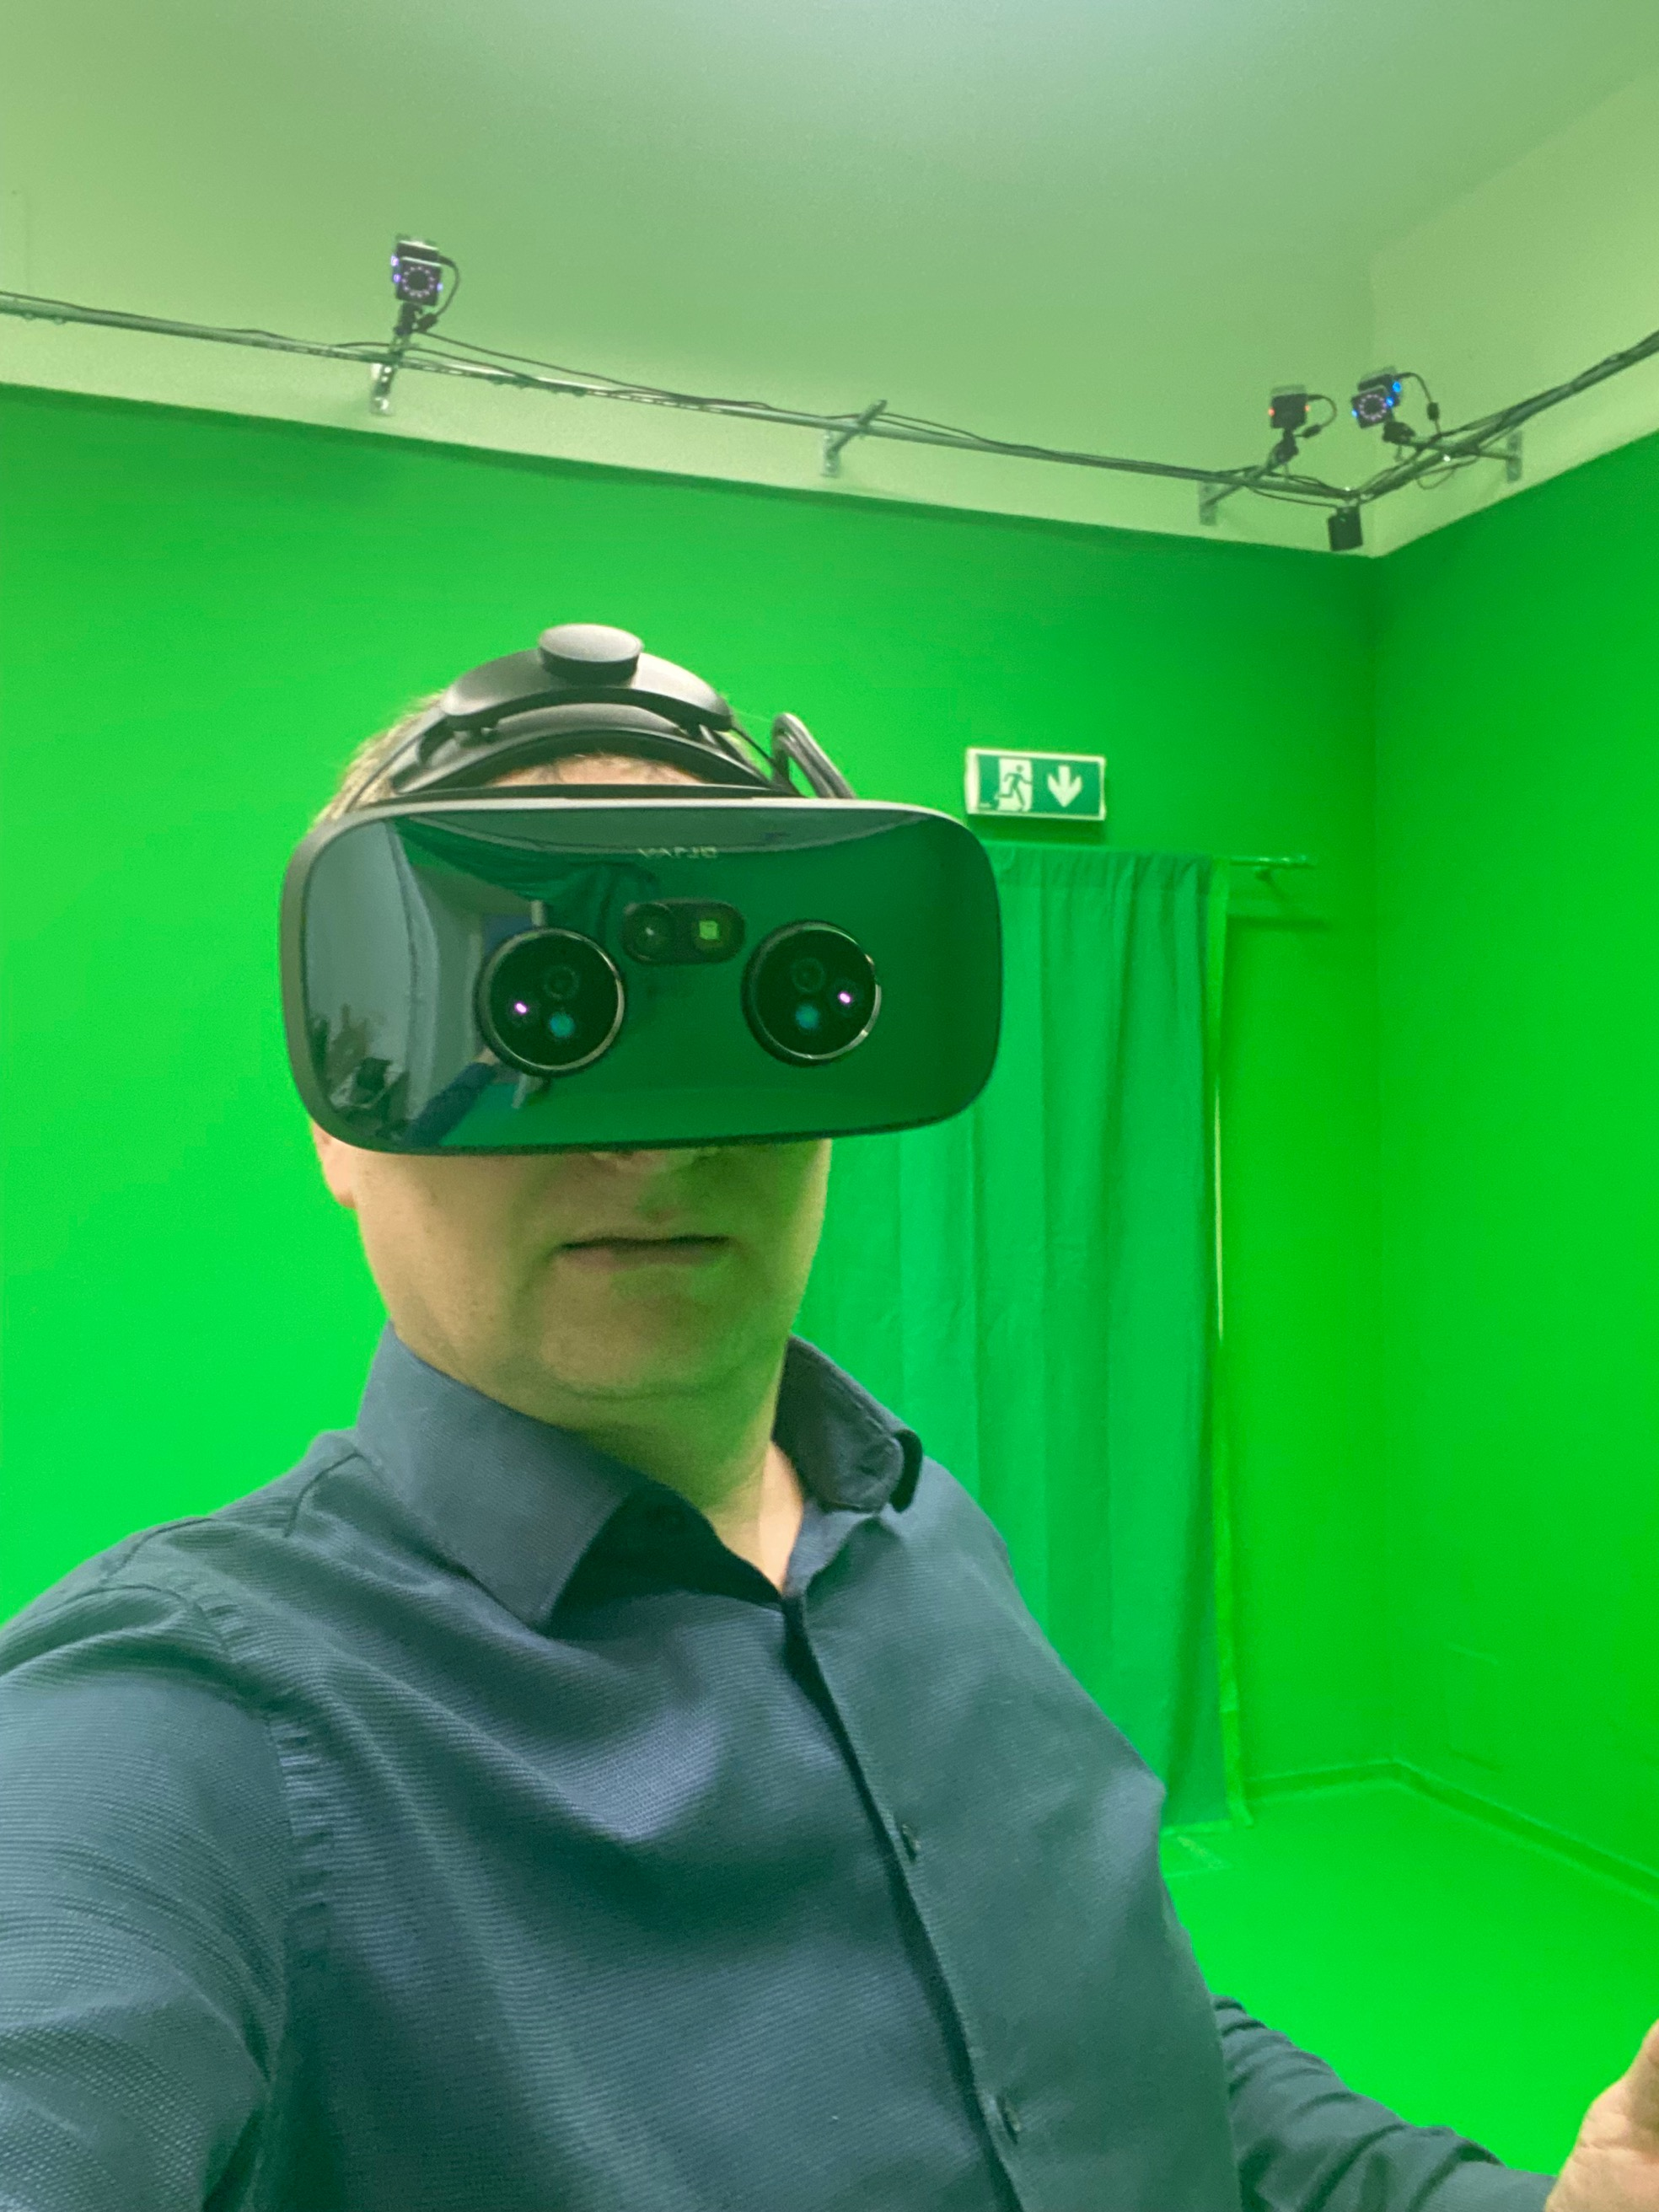
\includegraphics[width=0.89\textwidth]{img/ivr-supervisor.png}
        \caption{Varjo XR-3 headset in use.}
        \label{fig:ivr-sup}
    \end{subfigure}
    \hfill
    \begin{subfigure}[b]{0.6\textwidth}
        \centering
        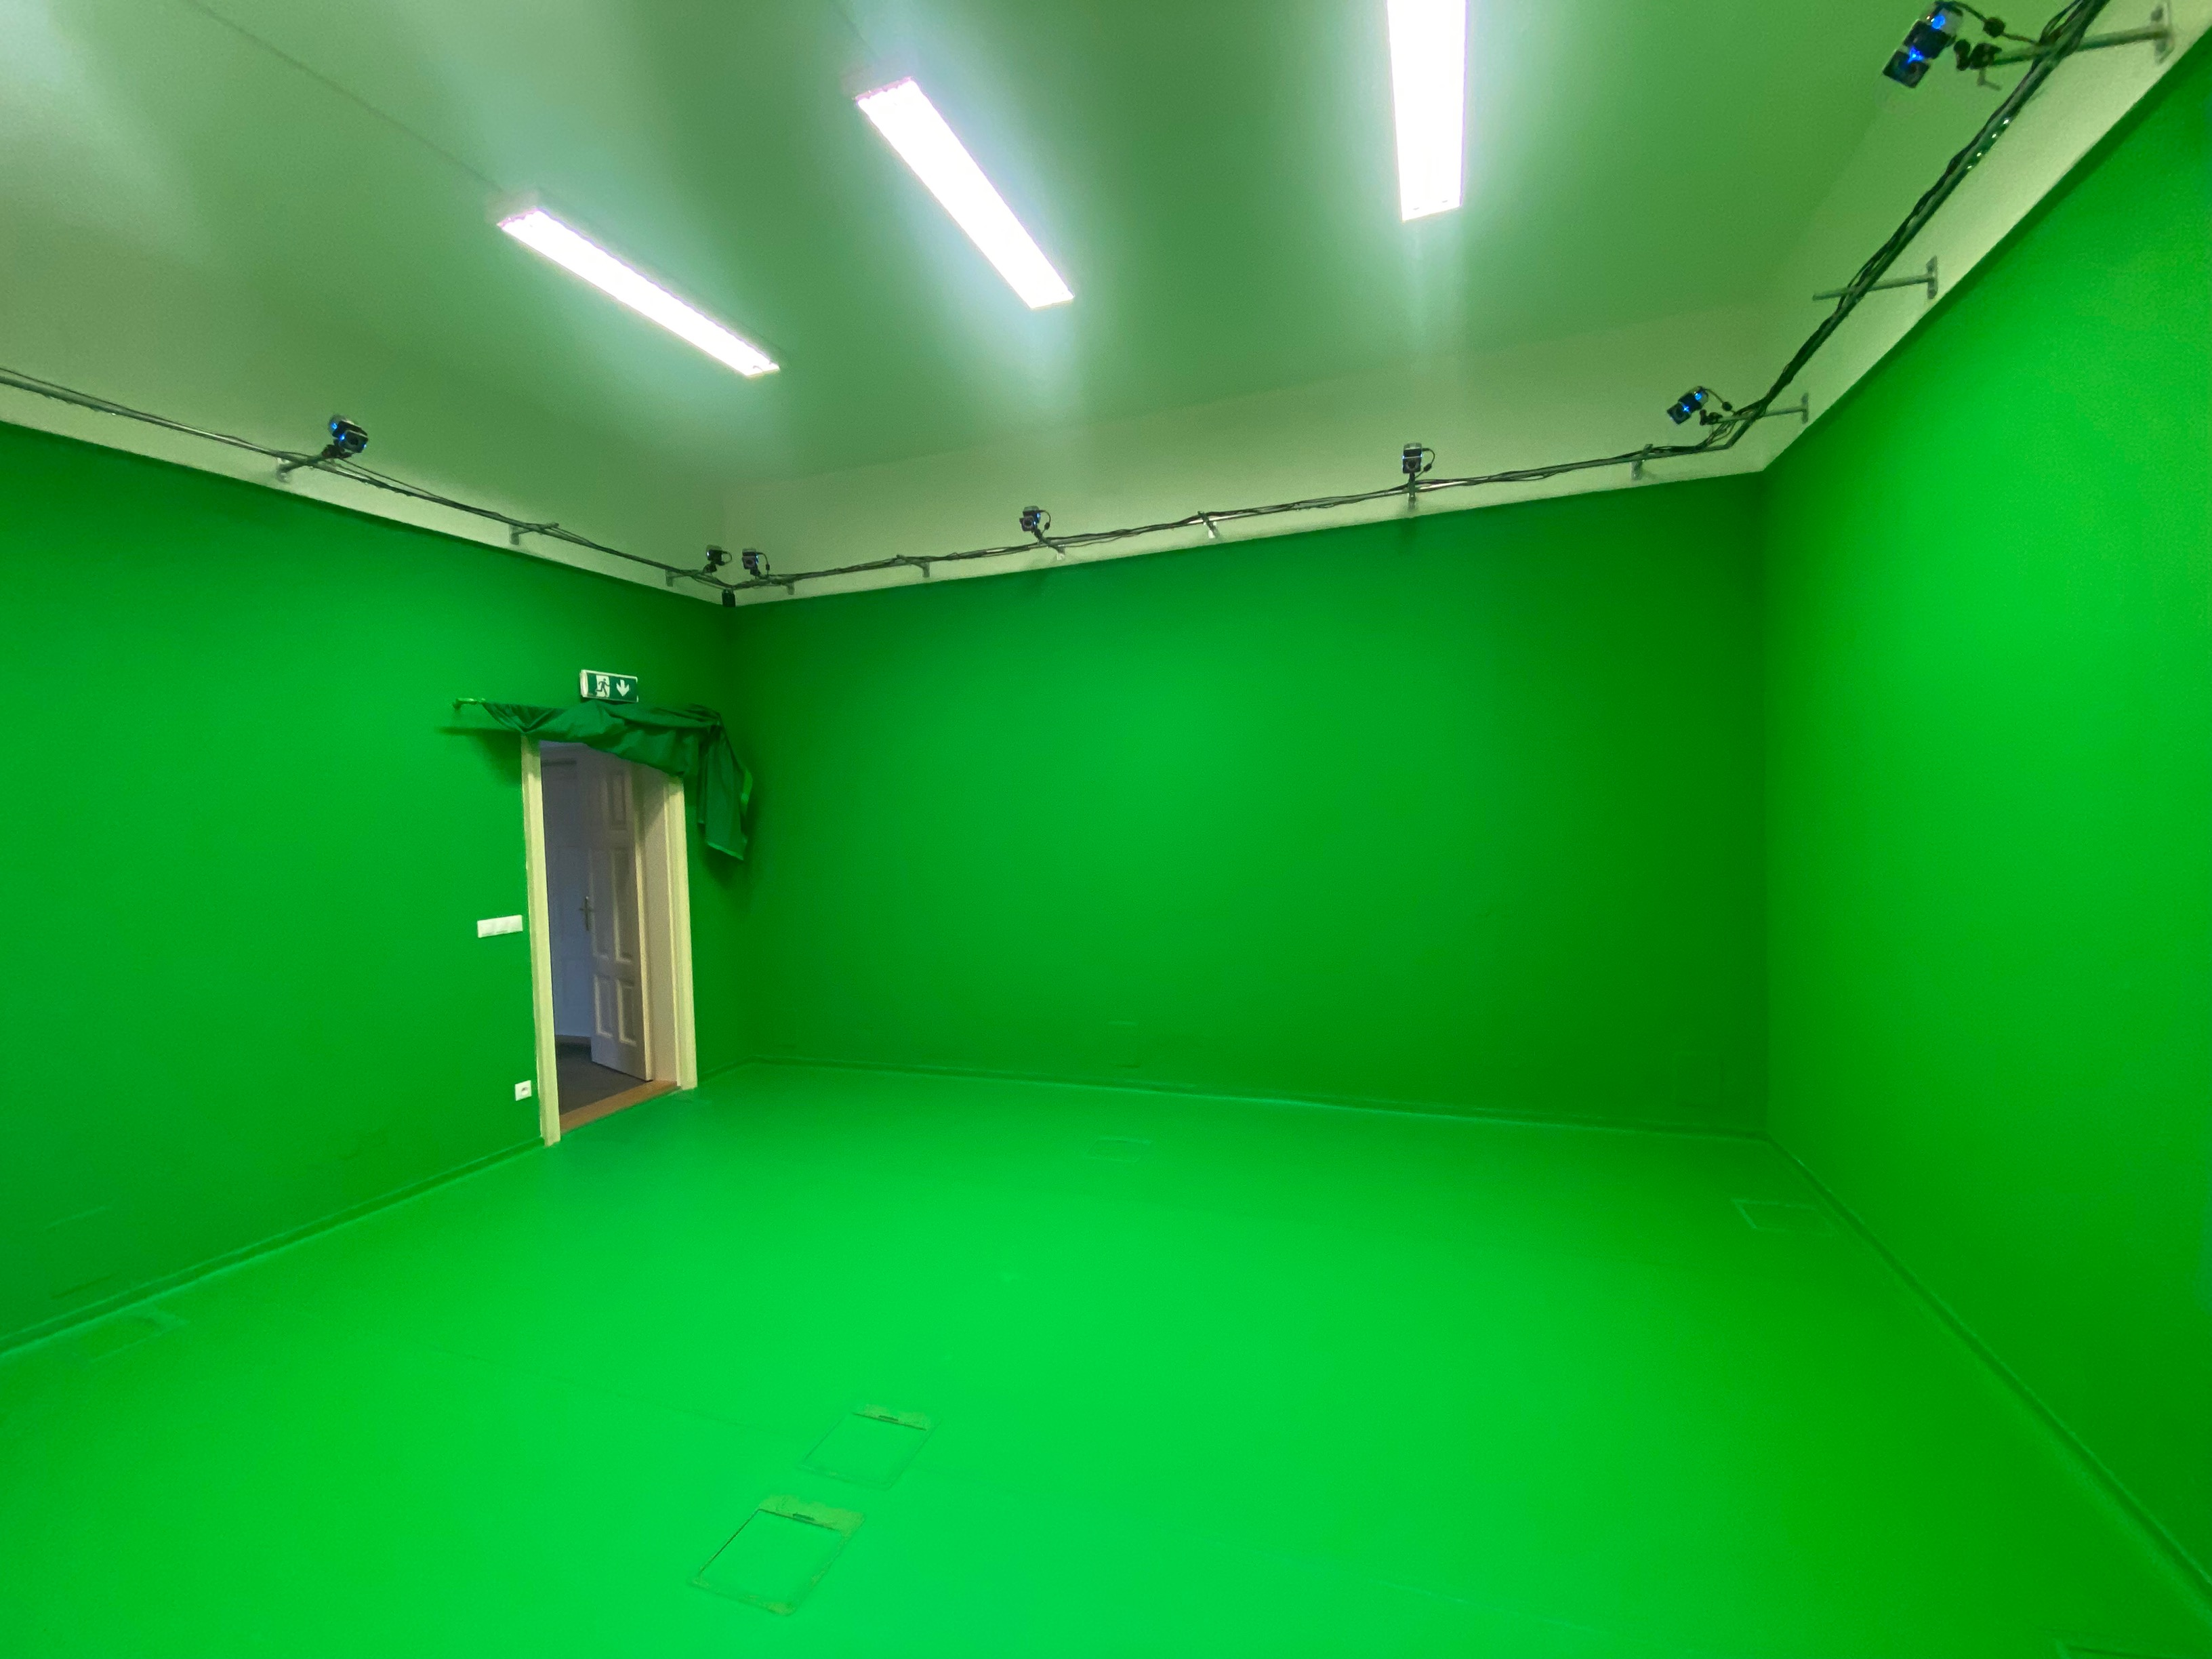
\includegraphics[width=\textwidth]{img/ivr-lab.png}
        \caption{Interiour of the~laboratory.}
        \label{fig:ivr-lab}
    \end{subfigure}
    \caption{Mixed reality laboratory for religious studies in Olomouc Palacký University.}
\end{figure}

This Czech lab uses the~aforementioned XR headset and its ET capabilities to~record and study human behaviour during religious processes. The~headset records a~video of the~lab, and then the~green screen is keyed out during the~post-process. The~result is used to~overlay the~virtual scene that is displayed later inside the~headset. They use VICON's tracking system to~track the~position of the~headset. The~system uses a~multiple camera setup, some of which can be seen in Figure~\ref{fig:ivr-lab}.

\subsection{Vrgineers XTAL}
\label{sec:xtal}

Vrgineers is a~Czech-American company that has been making VR headsets since 2016. Their hardware is called XTAL, and all of its versions include built-in ET hardware. The~latest XTAL is in version 3~\cite{vrginners-xtal3-spec}, Figure \ref{fig:vrg-xtal3}, which also exists in a~version for XR that includes additional cameras that project the~outside world inside. 

\subsubsection*{Features}
Headsets consists of several features. They offer auto-IPD, hand tracking with the~help of Ultraleap cameras, and an~ET system that consists of two arrays of several IR light dots, one for each eye, to~which a~single IR camera is paired. An~IR camera has a~resolution of 1280x800 pixels, which is captured at 110~Hz frequency. ET operates natively at 120~Hz, but it is possible to~increase the~frequency of the~eye tracker's output data up to 210~Hz.~\cite{vrginners-xtal-spec}

\subsubsection*{Runtime}
At the~time of writing, the~XTAL headsets communicated only using their stable native VRG runtime, which uses this ET system only for IPD measurement and foveated rendering. This was not entirely clear at the~beginning of the~investigation and was believed to be capable of returning gaze data because the~source code of their SDK included gaze data structures similar to those presented in Section~\ref{sec:gaze-data}. However, Vrgineers support later informed that they were developing another runtime that was capable of this.

Their~goal is to~convert the~entire native runtime to~OpenXR, which is currently in beta and already offers left, right, and combined gaze data according to the~OpenXR specification. The~native runtime offer support for native C development and integration to Unreal and Unity. They tested the~beta OpenXR runtime on Unreal Engine versions 4.27 and 5.~\cite{vrginners-email}

\begin{figure}[!t]\centering
    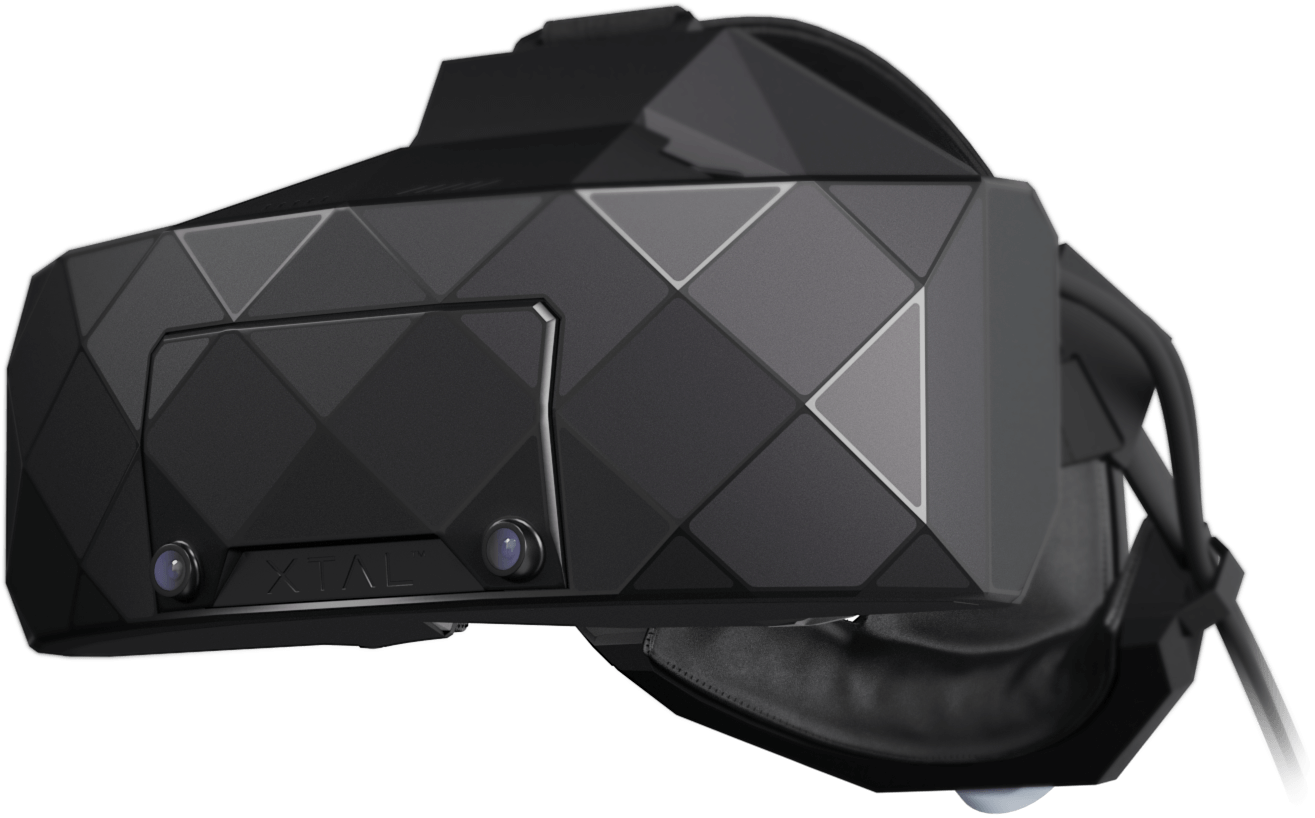
\includegraphics[width=0.6\textwidth]{img/xtal3.png}
    \caption[VRGineers XTAL 3 VR headset.]{VRGineers XTAL 3 VR headset.~\cite{vrgineers-xtal3-image}}
    \label{fig:vrg-xtal3}
\end{figure}

\subsubsection*{Eye tracker specification}
In this Bachelor's thesis written under the~Faculty of Electrical Engineering, CTU in 2020, a~prototype of eye detection and gaze estimation using the~ET system of the~XTAL headset was implemented. The~author used the~dark pupil method to~detect the~eyes by scanning the~pupil in the~recorded eye images. Gaze estimation was performed using a~2D regression method.~\cite{trnka2020thesis}

At this point, it is not clear whether the~ET implementation from the~Bachelor's thesis is present in the~current driver or if it has undergone significant changes. It is unrealistic to~assume the~accuracy of the~measuring algorithm because the~manufacturer has not yet provided it. 

ET does not work in XTAL without calibration. While a~VR application is running, one of the~two calibration options in the~VRG runtime must be triggered. The~faster one is the~one point calibration, which is used to~measure the~PID and enable foveated rendering, but can also be used to~enable ET itself. This option uses for calibration a~virtual mathematical model of the~user's face. For more accurate results of the~measured gaze data, the~more advanced calibration, consisting of seven points, should be used.~\cite{vrginners-xtal3-intro, vrginners-email}

\subsubsection*{XTAL VR Training}

Vrgineers has partnered up with the~U.S. Air Force to~build custom simulators for training fighter pilots. The~simulator can be seen in Figure~\ref{fig:vrg-cockpit}. When the~pilots sit inside, they have the~XTAL 3 XR headset on. This is an~example of VR training that mimics the~environment of various fighters such as F-15, F-18, and F-35 as closely as possible to~train muscle memory and situational awareness of pilots.~\cite{vrginners-classroom}


\subsubsection*{3D CAVE}
The~room with CAVE 3D is a~laboratory of the~Faculty of Mechanical Engineering of CTU. It consists of a~multiprojection system called CAVE, which is used to visualise scenes and scientific data. The~CAVE simultaneously projects stereoscopic images onto four cube faces; the~front, right, and left walls with the~floor, Figure~\ref{fig:cave-proj}. More specifically, it is used to display and verify virtual prototypes, where real physical parts of the~structures are compared to the~virtual prototype.~\cite{cave-lab}

The~very second part of this lab is a~corner with four XTAL headsets that run the~same application as the~projection system. The~headset can be walked around the~lab by attaching it to an~HP backpack. Figure~\ref{fig:cave-xtal}.

\begin{figure}[!ht]\centering
    \begin{subfigure}[b]{0.48\textwidth}
        \centering
        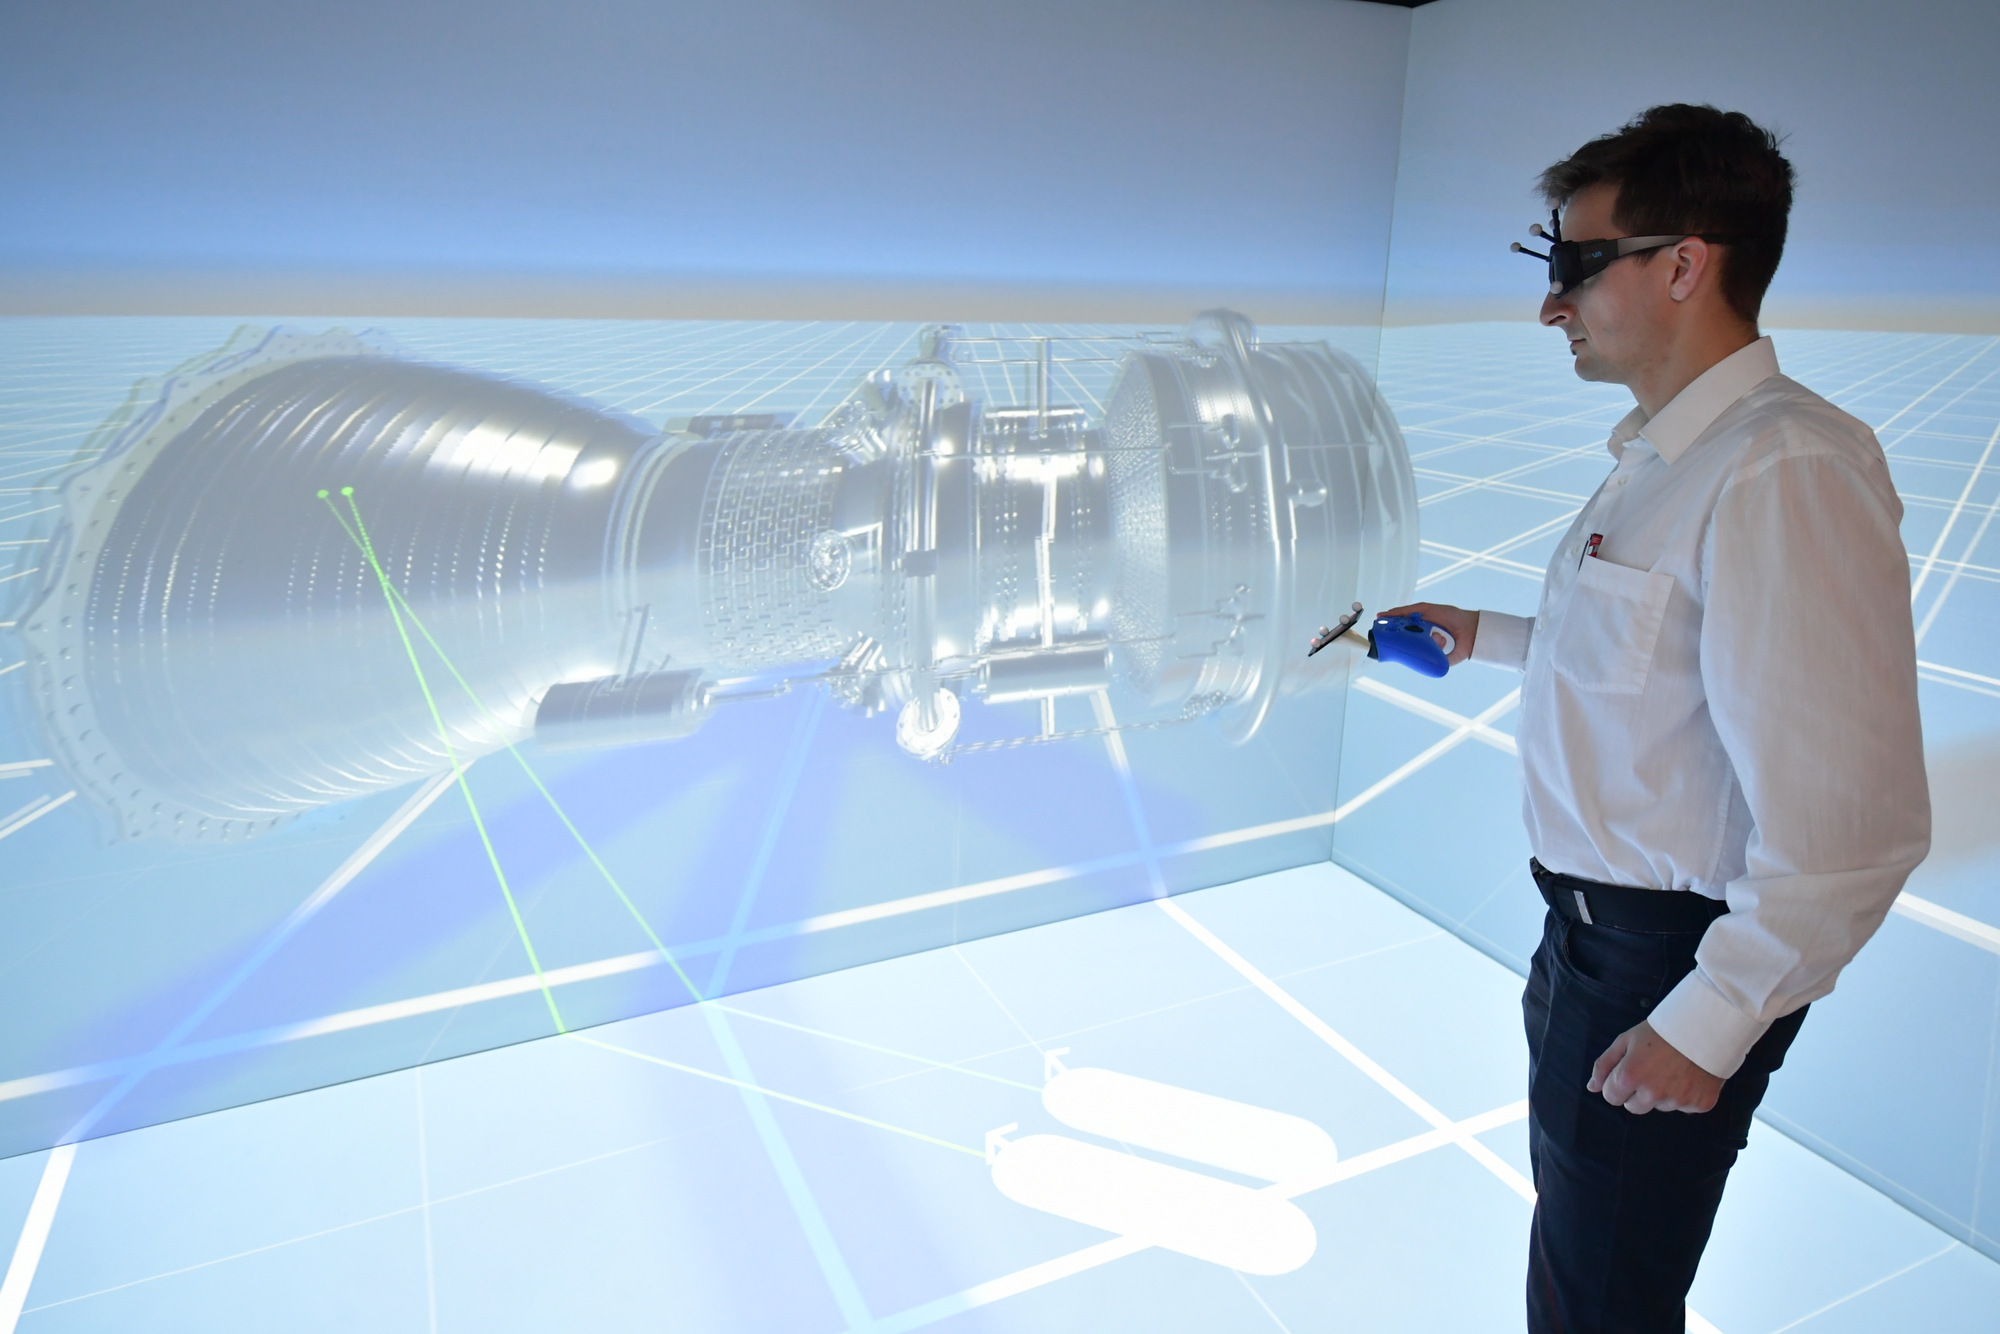
\includegraphics[width=\textwidth]{img/cave-projection.jpg}
        \caption{CAVE 3D multi-projection system.}
        \label{fig:cave-proj}
    \end{subfigure}
    \hfill
    \begin{subfigure}[b]{0.48\textwidth}
        \centering
        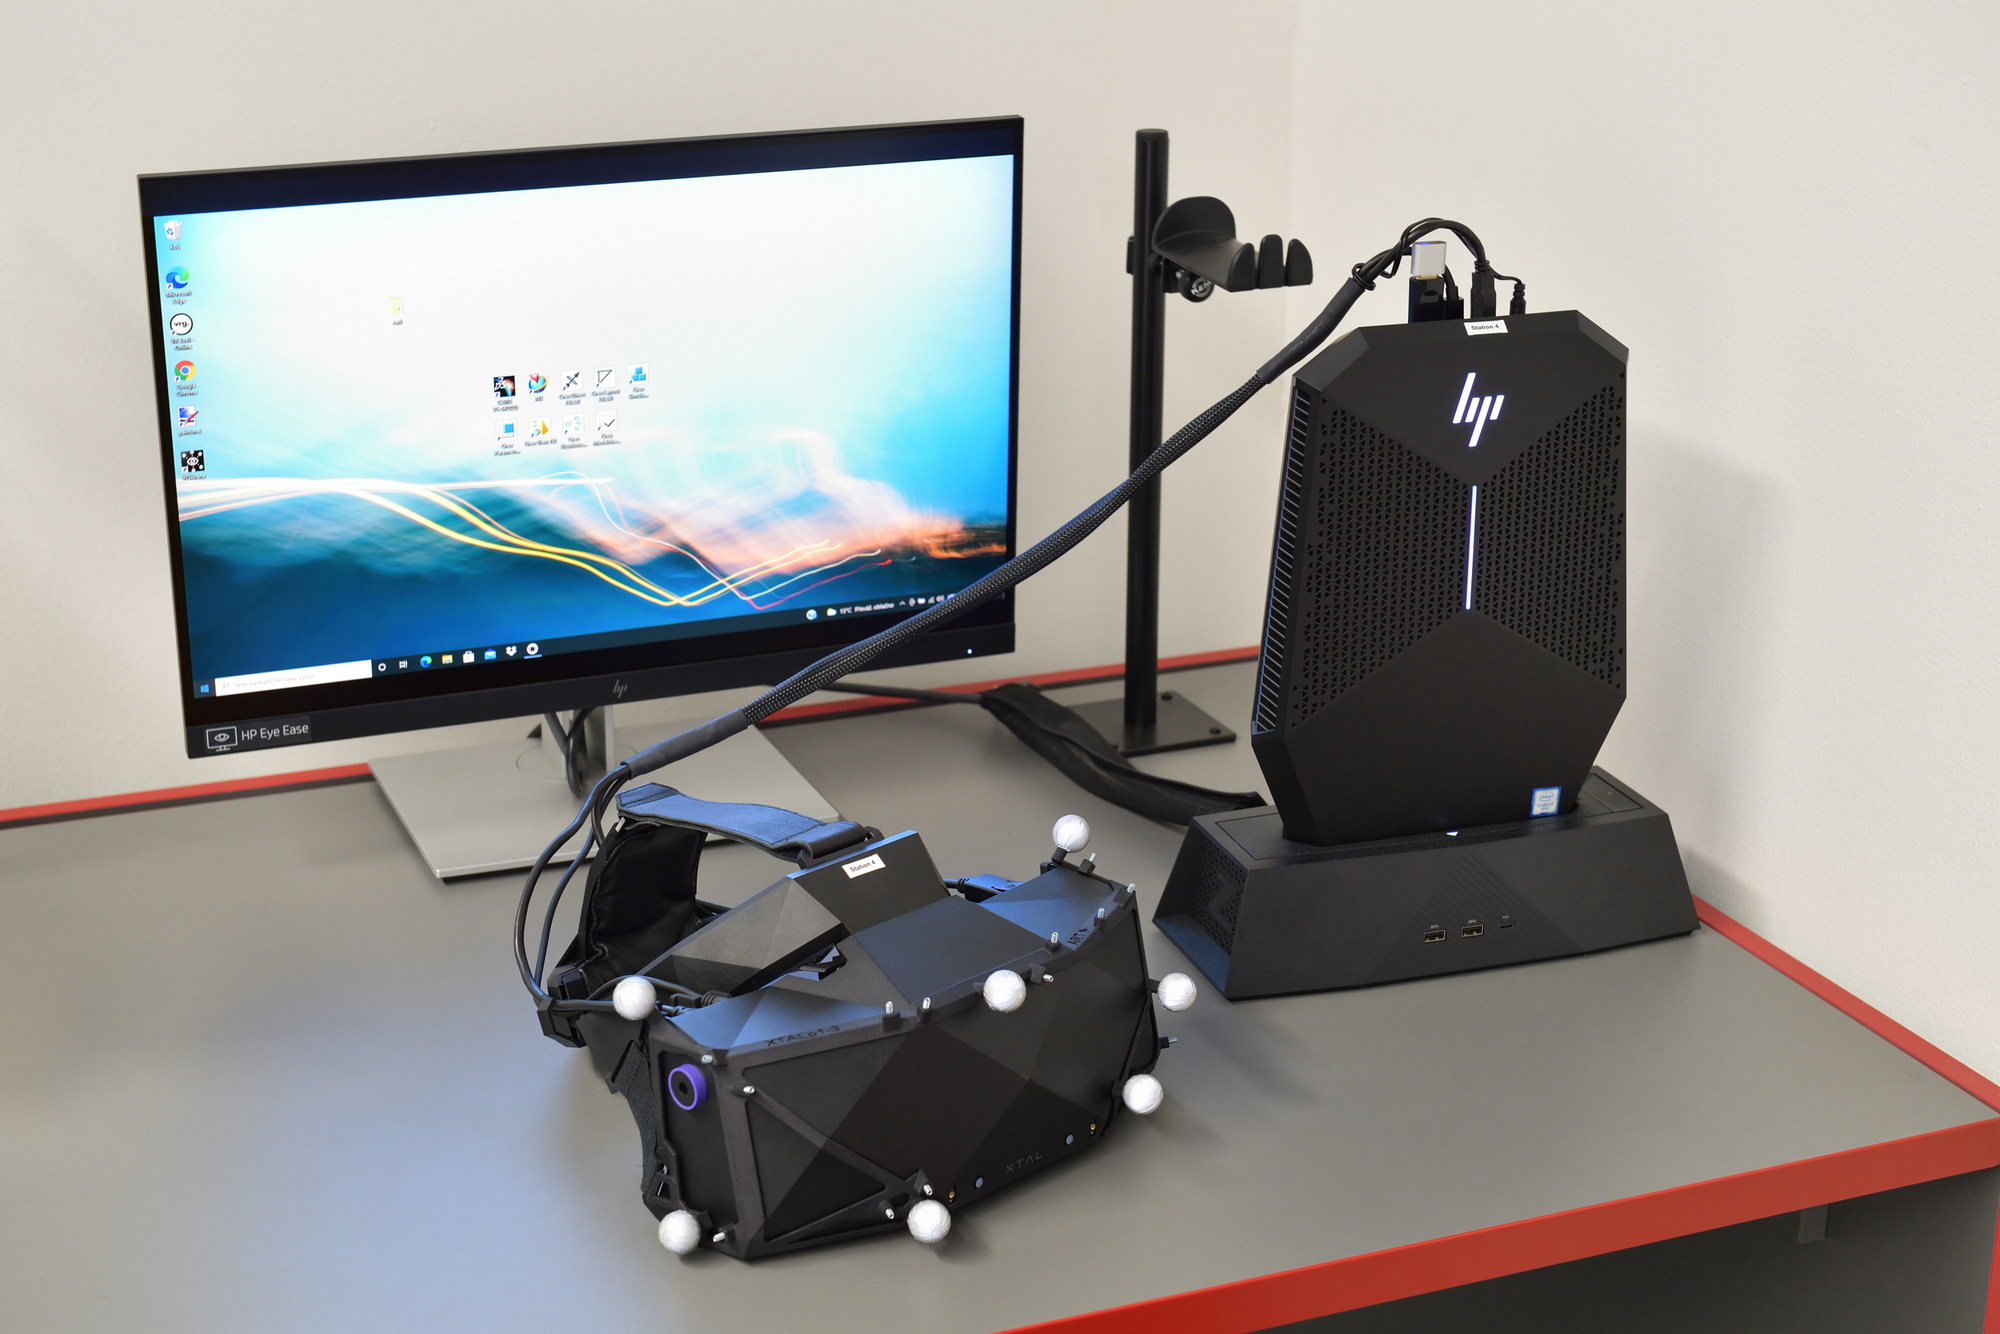
\includegraphics[width=\textwidth]{img/cave-xtal.jpg}
        \caption{XTAL with HP backpack.}
        \label{fig:cave-xtal}
    \end{subfigure}
    \caption[3D CAVE laboratory at CTU FME.]{3D CAVE laboratory at CTU FME.~\cite{cave-lab}}
\end{figure}


\begin{figure}[!ht]\centering
    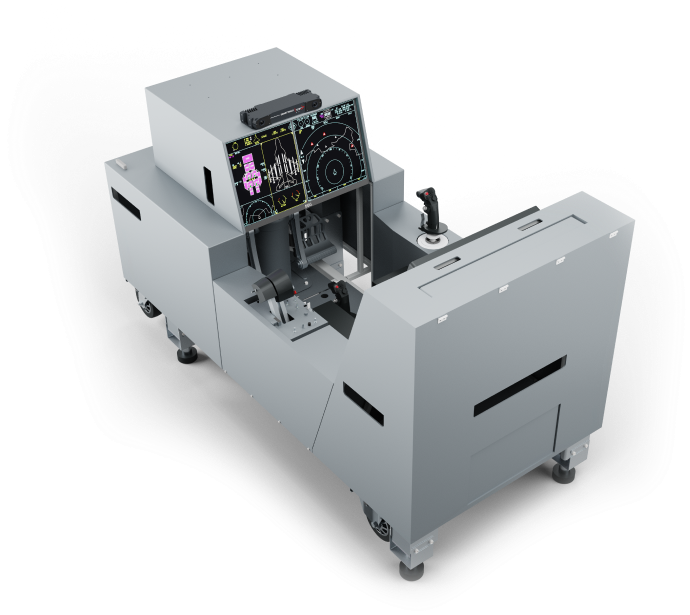
\includegraphics[width=0.5\textwidth]{img/xtal-cockpit.png}
    \caption[VRGineers fighter jet cockpit simulator.]{VRGineers fighter jet cockpit simulator.~\cite{vrgineers-cockpit}}
    \label{fig:vrg-cockpit}
\end{figure}

\subsection{Future possibility}

Another headset currently in development is the~successor to the~Playstation VR headset, which is designed for the~PS5 console; the~PSVR2. A~huge advantage of the~original version was that it was one of the~most affordable VR headsets on the~market. It admittedly did not have the~best specifications, but it did not cost more than \$400 when it was released. Compared to the~other headsets that could be purchased for at least double that amount. Although the~headset was made to be used exclusively on a~Playstation platform, it is possible to~communicate with it on a~PC via unofficial drivers.

The~new PSVR2 has dramatically improved technical specifications over its predecessor. The~internal OLED panel offers 2000x2040 pixels for each eye with a~refresh rate of up to 120~Hz, and an~FOV of 110 degrees. Most interestingly, it includes an~eye tracker. Sony's implementation will likely be proprietary to~keep the~cost as low as possible. The~setup is conventional with IR illuminators and one IR camera for each eye. The~main reason they want to~implement ET is to~add additional input for new games and for the~foveated rendering capability, which is mainly to~free up PS5 rendering performance. It~should offer developers of new PSVR games access to the~same gaze data structure as the~previous ET headsets.~\cite{psvr2, psvr2-specs}

Sony has not yet announced the~price of the~PSVR2 at the~time of writing this thesis, but it is rumoured that it will be around the~retail price of PS5, which based on the~announced specifications would be a~great bargain. The~question is whether Sony will develop an~official PC driver for it, or if there will be an~unofficial one that will for example communicate with this headset according to the~OpenXR standard. If so, the~headset would become the~cheapest VR headset with ET on the~market capable of being used for ET research.

\section{Existing solutions}
\label{sec:solutions}

This section summarises the~available solutions that use a~VR headset to~collect and visualise ET data with the~requirement of using game engines. Given how advanced modern ET hardware is, the~number of software implementations that use it is scarce. The~main player is Cognitive3D, which was the~first to~produce a~robust solution that addresses this and does so using current game engines.

The~Master's thesis written at the~Faculty of Informatics of Masaryk University in 2020 explored the~possibilities of ET technology in the~context of VR, where the~student designed and implemented a~software solution to~record, analyse, and visualise gaze data in~Unity with the~use of the~HTC VIVE Pro Eye headset for VR~\cite{ugwitz2020thesis}. The~solution was used for a~user study exploring escape behaviour. The~student did not evaluate the~gaze data in real time but first collected them into an~external CSV file, which was later analysed. To~visualise these data, he used visual indicators that were assembled from basic Unity primitives such as a~cube, a~sphere, or a~lineRenderer. Points of fixation (PoF) are visualised in the~thesis as concentrations of several ET points in a~3D space, which are coloured by a~white-to-pink gradient that is supposed to~liken them to~heatmaps.

\subsection{Cognitive3D}
Cognitive3D is a~company based in Vancouver, Canada, that offers an~entire proprietary system made up of several parts for the~collection and analysis of ET data. The~system includes a~streamlined production of use-case scenarios that are defined using objectives. The~system can also be used for VR environments that do not employ ET in any way. It~is applicable to~academic and marketing research, VR training simulation, or architectural design. It~has been designed to~allow any content from Unreal or Unity to~be integrated into the~system using the~corresponding \emph{plug-in}. The~\emph{plug-in} takes control of the~entire scene in an~engine. The~annual academic licence is in the~range of tens of thousands of dollars.~\cite{cognitive3d-splash, cognitive3d-meeting}

\pagebreak{}


% \begin{figure}[!ht]\centering
%     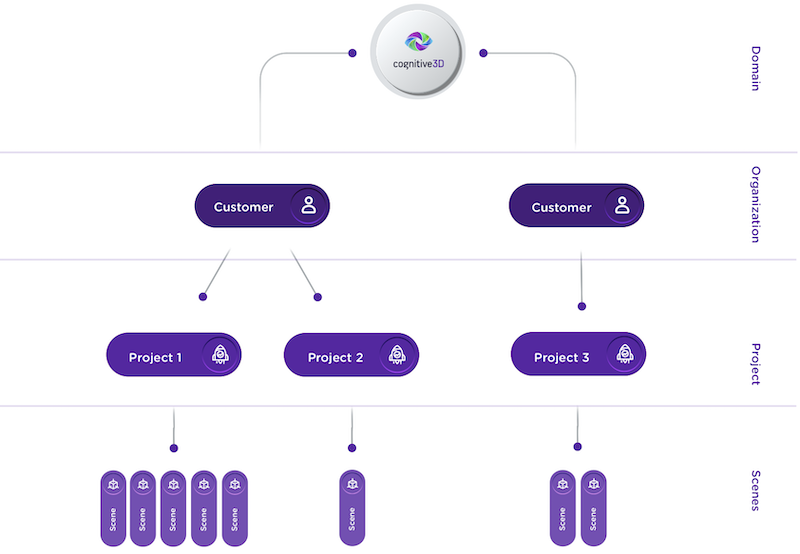
\includegraphics[width=0.8\textwidth]{img/cognitive3D-platform-hierarchy.png}
%     \caption[Cognitive3D platform hierarchy.]{Cognitive3D platform hierarchy.~\cite{cognitive3d-dashboard-concepts}}
%     \label{fig:cognitive3d-platform}
% \end{figure}

\subsubsection*{Dashboard}
The~application that holds the~whole platform together is called Dashboard. It is a~web interface that contains several different functions and handles the~structure of multiple users/organisations and their projects.~\cite{cognitive3d-dashboard-concepts}

A~\emph{customer} is an~entity with a~paid licence that can create various projects. Each \emph{project} can have multiple defined \emph{scenes}, which are containers for static scene geometry, \emph{dynamic objects} and \emph{session} data. A~\emph{session} is a~specific instance of a~single participant measurement that collects session data during the~runtime of a~Cognitive3D application that contains a~scene of an~experiment.

\subsubsection*{SceneExplorer}
One of the~main functions of the~Dashboard is the~SceneExplorer, which is used for a~detailed review of the~participant's session. This session contains a~timeline that stores all actions, events, user movements and gazes, and fixations on objects performed during an~experiment. The~timeline can be stopped at any time to~explore the~state of the~scene. It can display exactly where the~participant was looking. The~gaze is visualised as a`heatmap that fades according to a~time fall-off. Fixation points are displayed using a~trail consisting of spheres (fixations) and lines (saccades).~\cite{cognitive3d-scene-explorer}

\subsubsection*{Gaze and Fixations}
Cognitive3D can be used without an~ET headset, but in this case fixations and their metrics cannot be collected during the~experiment, only gaze, which is collected based on the~virtual position of the~HMD. Gaze metrics are recorded always, but without an~eye tracker the~application assumes that the~participant's focus is directly in front of the~HDM. In this case, the~metrics are significantly less accurate.~\cite{cognitive3d-unreal-gf}

\begin{table}[!ht]
\begin{tabular}{|c|l|}
\hline
Metric &
  Description \\ \hline\hline
\begin{tabular}[c]{@{}c@{}}Average Gaze Count\end{tabular} &
  \begin{tabular}[c]{@{}l@{}}The~average number of times someone gazed at the~object during\\ one session.\end{tabular} \\ \hline
\begin{tabular}[c]{@{}c@{}}Average Gaze Time\end{tabular} &
  \begin{tabular}[c]{@{}l@{}}The~average time the~object was gazed at during one session.\end{tabular} \\ \hline
Gaze Ratio &
  \begin{tabular}[c]{@{}l@{}}Reports the~percentage of sessions in which the~object was gazed at.\end{tabular} \\ \hline
\begin{tabular}[c]{@{}c@{}}Total Sessions\\ with Object\end{tabular} &
  \begin{tabular}[c]{@{}l@{}}The~number of times the~object was present in a~session.\end{tabular} \\ \hline
\begin{tabular}[c]{@{}c@{}}Total User Gazes\\ at Object\end{tabular} &
  The~total number of all gazes. \\ \hline
\begin{tabular}[c]{@{}c@{}}Sessions with\\ Gaze\end{tabular} &
  \begin{tabular}[c]{@{}l@{}}The~number of sessions in which the~participant noticed the~object\\ at least once.\end{tabular} \\ \hline
User Gaze Length &
  The~total duration of all gazes. \\ \hline
\begin{tabular}[c]{@{}c@{}}Gaze Instance\\ Duration\end{tabular} &
  The~average duration of one instance of gaze. \\ \hline\hline
Gaze Sequence &
  The~sequence of all objects that were seen earlier. \\ \hline
Time to Gaze &
  \begin{tabular}[c]{@{}l@{}}The~duration from the~beginning of the~session to the~first gaze of\\ the~object.\end{tabular} \\ \hline
\end{tabular}
\caption[Cognitive3D gaze metrics of dynamic objects.]{Cognitive3D gaze metrics of dynamic objects.~\cite{cognitive3d-metrics}}
\label{tab:cognitive3d-metrics}
\end{table}

\pagebreak{}

\begin{table}[!ht]
\centering
\begin{tabular}{|c|l|}
\hline
Metric &
  Description \\ \hline\hline
Completions &
  The~number of users that completed the~step. \\ \hline
\begin{tabular}[c]{@{}c@{}}Completions in \%\end{tabular} &
  \begin{tabular}[c]{@{}l@{}}Total number of completions compared to\\ the~total amount of sessions.\end{tabular} \\ \hline
\begin{tabular}[c]{@{}c@{}}Average Step Duration\end{tabular} &
  \begin{tabular}[c]{@{}l@{}}The~average time to complete the~step relatively to\\ the~previously completed step.\end{tabular} \\ \hline
\begin{tabular}[c]{@{}c@{}}Average Step\\ Completion Time\end{tabular} &
  \begin{tabular}[c]{@{}l@{}}The~average time to complete the~step relatively to\\ the~session start.\end{tabular} \\ \hline\hline
\begin{tabular}[c]{@{}c@{}}Successful Sessions\end{tabular} &
  \begin{tabular}[c]{@{}l@{}}Total number of sessions that have cleared\\ successfully every step.\end{tabular} \\ \hline
Total Sessions &
  \begin{tabular}[c]{@{}l@{}}Total amount of sessions with the~same objective.\end{tabular} \\ \hline
\begin{tabular}[c]{@{}c@{}}Success Rate in \%\end{tabular} &
  \begin{tabular}[c]{@{}l@{}}The~total number of successful sessions compared to\\ total sessions.\end{tabular} \\ \hline
\end{tabular}
\caption[Cognitive3D metrics used for objectives and its steps.]{Cognitive3D metrics used for objectives and its steps.~\cite{cognitive3d-metrics}}
\label{tab:cognitive3d-obj-metrics}
\end{table}

Gaze and fixation metrics are aggregated for individual dynamic objects that represent regions of interest (RoIs) in the~scene. A~group of several objects can be defined and treated as a~separate RoI. Both metrics have the~same structure, but their description is presented only on~gaze metrics~\cite{cognitive3d-dynamic-objects}. The~Table~\ref{tab:cognitive3d-metrics} shows gaze metrics that are collected for each object independently over all sessions of a~given scene. The~last two metrics are collected only in the~context of a~single session.~\cite{cognitive3d-metrics}

\subsubsection*{Objectives}

The~next main functionality of the~Cognitive3D software are the~objectives, which are composed of individual steps and thus represent a~certain script of what should occur during a~session. They allow to~collect information about what the~participant was able to~complete within a~session or if they followed a~certain process. Any~amount of objectives can be defined in the~context of a~scene, and any amount of these objectives can be assigned to a~session. An~example of one with a~list of individual steps and their calculated results in the~Dashboard web interface can be seen in Figure~\ref{fig:cog3d-steps}, and Figure~\ref{fig:cog3d-obj} displays the~dialogue box in which the~criteria of a~single step for its completion are set.~\cite{cognitive3d-objectives}

\begin{figure}[!ht]\centering
    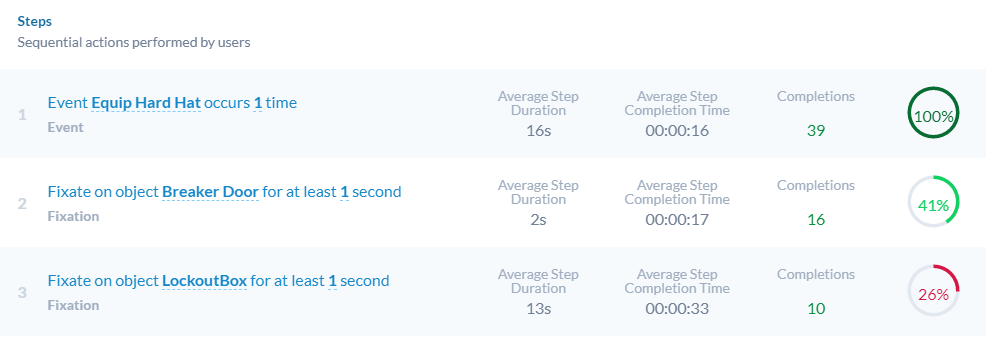
\includegraphics[width=\textwidth]{img/cognitive3D-steps.png}
    \caption[Sequence of steps and their completion in Cognitive3D.]{Sequence of steps and their completion in Cognitive3D.~\cite{cognitive3d-objectives}}
    \label{fig:cog3d-steps}
\end{figure}

\pagebreak{}
Registering whether a~step was successful can be easily evaluated using ET by whether the~participant fixated or gazed at a~particular object. A~step of an~objective is considered to be completed if it meets the~specified criteria. It is possible to set the~number of required fixations or their duration. Using this input, the~first four metrics shown in Table~\ref{tab:cognitive3d-obj-metrics} are collected for each step; the~same metrics can be seen in Figure~\ref{fig:cog3d-steps}. The~remaining three metrics of Table~\ref{tab:cognitive3d-obj-metrics} are collected for the~objective as a~whole. 

\begin{figure}[!t]\centering
    \includegraphics[width=0.7\textwidth]{img/cognitive3D-objective.png}
    \caption[Setup of a~step in Cognitive3D that activates at gaze.]{Setup of a~step in Cognitive3D activating at gaze.~\cite{cognitive3d-objectives}}
    \label{fig:cog3d-obj}
\end{figure}

\subsubsection*{Supported hardware}
The~system is built to~be compatible with a~wide range of devices. It offers a~high number of VR devices without ET. Among the~VR HMDs with ET, it supports all of the~previously mentioned with Tobii eye tracker in Section~\ref{sec:integrations} and all Varjo headsets in Section~\ref{sec:varjo}. Support for XTALs did not exist during the~writing of the~thesis.

\section{Unreal Engine capabilities}

\emph{Unreal Engine} (UE), developed by Epic Games~\cite{unreal-engine}, is used to render 3D computer graphics in real time. First designed for game development, it has found use in many other industries. Engine development is possible in C\texttt{++} or using \emph{Blueprint Visual Scripting}. This section first briefly introduces the~tools used for development inside the~engine~\cite{unreal-documentation} and the~options on how to process gaze data for heatmap production in real time.

\subsection{Blueprint Visual Scripting}
\emph{Blueprint}, short for \emph{Blueprint class}, is based on a~node-based interface to create, modify, and control elements in an~Unreal scene. It is essentially a~class that is stored as an~Asset in the~Content Browser. It allows designers to use programming tools without having to touch the~C\texttt{++} language. 

Any functionality that Blueprints do not offer can be programmed using C\texttt{++} and then made available to Blueprint nodes. A~Blueprint does not have to contain a~functionality for a~specific gameplay element. It can exist fully independently as a~collection of static functions. It is called \emph{Blueprint Function Library}. Unreal Engine already comes with a~rich set of tools that define many Blueprint classes and libraries. Many Blueprint classes can be used as a~parent class for new ones that inherit their functionality.

\subsection{Tools and Classes}
For this thesis, it is crucial to know these UE options. The~scale of an~UE scene is defined in centimetres.

\begin{description}
    \item[Asset] is a~piece of content, the~engine can work with, that is located in Content Browser; part of Unreal's interface. Assets are files stored with \path{.uasset} extension. They represent, for instance, imported models and textures, or Blueprints.
    \item[Actor] is a~class that by default maintains 3D spatial information about its position and rotation, which can always be modified. An~Actor is spawnable and destroyable at any time. It can be, for example, a~controlled character, cameras, lights, or other 3D models. Each Actor in a~scene has its own Blueprint and a~\emph{Component graph}; hierarchical tree of Components.
    \item[Pawn] is an~Actor that is the essential physical representation of a~player within the~world. It is the~base class for all Actors that can be controlled either by a~player or an~AI. It is possible to add a~DefaultPawnMovementComponent to a~pawn to extend it with simple no-gravity movement.
    \item[Character] is a special type of Pawn that offers basic movement abilities for vertically orientated characters that can walk, run and jump.
    \item[Component] is a~Blueprint class that provides functionality that is attachable to any Actor at any time. 
    \item[Level] is a~special type of Asset that serves as a~hierarchical collection of several different Actors to create a~scene. Each Level in a~project has one Blueprint assigned by default.
    \item[Tick] is defined within the~engine as a~regular interval that usually occurs once every frame. An~actor may have a~defined OnTick function that is repeated periodically. It is often used to update a~given Actor.
    \item[Material] is an~Asset that defines how a~surface should be rendered. It is defined using visual scripting nodes -- Material Expressions -- in the~Material Editor, which is not a~Blueprint. Each material is translated as an~HLSL programme executed on a~GPU consisting of a~vertex and a~pixel shader. The~nodes replace pieces of HLSL code.
    \item[Static mesh] is an~object class that represents the~fundamental renderable static geometry. It is generated by importing a~3D model into a~UE project. It can be edited in the~Static Mesh Editor, which includes, among other functions, collision, UV map, and LOD settings or Material~assignment. A~static mesh also exists as a~Component or an~Actor, which effectively contains a~StaticMeshComponent as the~root of its graph. The~mesh is rendered according to the~assigned material.
    \item[Material Instancing] is a~method that is used to change the~appearance of material without recompiling the~HLSL programme. Some Material Expression nodes such as vectors, textures and floats can be turned into parameters that are set before the~Material is rendered. This requires to construct a~Dynamic Material Instance of the~given Material.
    \item[Canvas Render Target 2D] is a~Blueprint object class that inherits Texture class. This is a~texture that can be constructed, modified, and exported at runtime.
    \item[Scene Capture 2D] is a~camera Component that captures a~scene from its position using its view frustum into a~texture. It can record the~scene continuously every Tick or just once by calling its Blueprint function \emph{Capture Scene}.
    \item[ShowOnly List] is an~option inside the~Scene Capture Component's settings that allows to render only those objects that are in the~list. This option must be explicitly enabled first.
    \item[Line Trace] is a~Blueprint function, callable only from an~Actor, that will perform trace collisions along a~specified 3D line; parameters Start and End. The~function returns the~first object hit by this line.
    \item[Plug-in] is a~collection of code or data that developers can enable or disable within their projects. Additional plug-ins are installed by placing them in the~project's Plugins directory or the~UE root directory in the~[Root]/Engine/Plugins folder.
\end{description}

\subsection{OpenXR}
There are different ways to interact with VR, XR, and AR devices in Unreal. However, it offers a~unified way to access them using OpenXR. To activate certain features, it is crucial to enable a~certain plug-in. Basic compatibility is guaranteed by the~OpenXR plug-in. Additional functionality can be activated by enabling OpenXRHandTracking and OpenXREyeTracker.

Due to potential conflicts and errors, it is recommended to disable other proprietary plug-ins designed to communicate with their hardware and other methods such as SteamVR, OculusVR, or Oculus OpenXR.

Unreal offers a~simple interface for ET, through which gaze data from OpenXR are sent when the~plug-in is enabled. \emph{Get Gaze Data} returns a~combined gaze, \emph{Get Stereo Gaze Data} returns two gazes, one for each eye. The~gaze data structure consists of an~origin and direction vector in the~absolute real world coordinates of a~tracking system used with the~headset. 

\subsection{UV mapping}
A~static mesh is a~geometric shape that remains unchanged and always contains the~same number of vertices and faces. The~way static meshes are rendered depends on their attached Material. Often these meshes are rendered with a~texture according to their UV maps.

\emph{UV mapping} is a~procedure in which a~2D image is projected onto a~3D model. For this to happen, it is necessary that the~3D model has its own UV map, which assigns to its vertices its own $(u, v)$ coordinate where $u,v$\,$\in$\,$[0, 1]$. A~texture or an~image has its width and height scaled to the~range of the~UV map during rendering. The~areas formed by connecting the~$(u, v)$ coordinates of the~vertices project the~corresponding piece of a~texture onto the~3D mesh itself.

\pagebreak{}
\subsection{Mesh painting}

Unreal offers the~ability to create dynamic textures using Render Targets and Dynamic Materials. Drawing on the~mesh itself can be simulated by modifying its texture. For this to work, the~UV map must not have overlapping faces defined. Each face of the~3D model must have a~uniquely assigned area in the~texture. This is also required by lightmaps in UE, which are used to bake scene lights into textures themselves, so they do not have to be computed during rendering.

In the~context of ET data visualisation, there is the~question of using mesh painting to produce heatmap textures based on a~gaze vector that collides with the~given object. Render Target can be exported in runtime.

It needs to be tested if this method of data collection is worth doing in real-time performance-wise, and how much storage it will require with multiple objects in the~scene -- each must have its own heatmap texture.

\subsection{UV painting method}

The~first approach to drawing heatmaps on textures would be to use a~collision hit position of the~object, which will be mapped to the~appropriate $(u, v)$ coordinate. This requires enabling the~Support UV From Hit Results option in the~Engine -- Physics section of the~UE project settings. 

This Unreal tutorial~\cite{texture-painting-tutorial} shows a~method for painting with a~brush defined using a~Material, which is set to additive blend mode. This is necessary to add new values to the~resulting Render Target instead of replacing them. 

\begin{figure}[!ht]\centering
    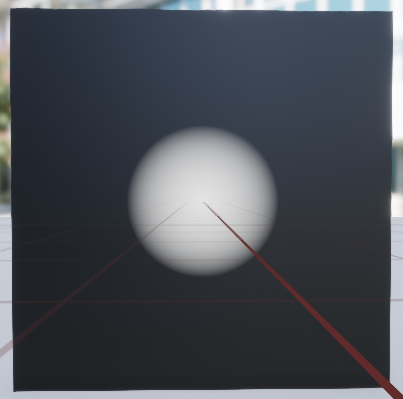
\includegraphics[width=0.4\textwidth]{img/Brush-material.png}
    \caption[Preview of 2D brush Unreal Material.]{Preview of 2D brush Unreal Material.~\cite{basic-heatmap-tutorial}}
    \label{fig:brush-material}
\end{figure}

The~brush material is shown in Figure~\ref{fig:brush-material}. The~appearance of the~preview corresponds to the~brush settings of $0.2$ radius and $(0.5, 0.5)$ coordinate on an~UV map. The~material has these values as input parameters that can be set before rendering to a~Render Target. As these parameters change, the~brush will change its position and size.

Render Target must be a~square texture that directly shadows the~UV map range. This texture is set to a~16-bit colour depth for each channel for greater detail of the~brush.

It is beneficial to first record the~heatmap as a~brush trail for easier manipulation of the~visualisation. One material can be seen in this Unreal tutorial~\cite{basic-heatmap-tutorial}. The~recorded trail can be displayed as a~heatmap on a~model using additional material that will be responsible for its appearance. The~parameters of the~Material are set by its Material Blueprint functions with the~wording \emph{Set Parameter Value}. A~Material is rendered to a~Render Target using the~Blueprint function \emph{Draw Material To Render Target}.

\subsubsection*{Problems}
There is however a~major drawback to this method. Brush splats are always drawn directly on a~texture. It does not reflect the~actual geometry and size of the~3D model in the~scene. The~UV map is not guaranteed to have all faces defined on the~same scale or aspect ratio. For such models, this would cause the~heatmap trail to be stretched for some faces or to be of a~different size. 

For symmetric, uniform, and unambiguous models with a~clearly defined UV map, such as a~cube or a~plane, this will certainly work much better. But it is also inadequate because it does not prevent brush overflow, where the~drawing stroke on a~certain face overflows into another. An example of this issue is demonstrated in the \path{video/01-basic-painting-method.mp4} in the enclosed DVD. The~wall model in the~video is a~single object. This solution is unsatisfactory and a~more suitable one is needed to address these problems.

\subsection{UV unwrap method}
\label{sec:uv-unwrap-method}

In this blog post~\cite{brucks2016shaderbits}, Unreal Engine veteran Ryan Brucks discusses automatic UV dilation to prevent edge bleeding for lower resolution mipmaps. In the~process, he also published his method for unwrapping meshes on the~basis of its UV map. The~first step in achieving dilation involves unwrapping the~model in the~world according to UV. The~object appears in the~scene as a~3D plane, which is rendered using an~orthographic Scene Capture Component to a~Render Target with a~32-bit pixel depth. In this texture, 3D coordinates of the~mesh's absolute position in the~world are captured. 

Dilation is then achieved by stretching the~faces' edges on the~UV map using algorithms that make use of other UE Materials. What is needed mainly for this thesis is the~unwrap method. Use a~brush that imprints itself on the~texture in the~exact areas around where a~gaze vector has hit the~object.

This requires using the~absolute world coordinates of the~mesh vertices while arranging the~vertices of an~object to appear on a~single unwrap plane that will be recorded in a~texture. The~way a~model looks when it is unwrapped can be seen in Figure~\ref{fig:unwrapped-mesh}, and how it is implemented in the~Material Expression nodes is shown in Figure~\ref{fig:unwrap-offset}. 

\begin{figure}[!ht]\centering
    \begin{subfigure}[b]{0.48\textwidth}
        \centering
        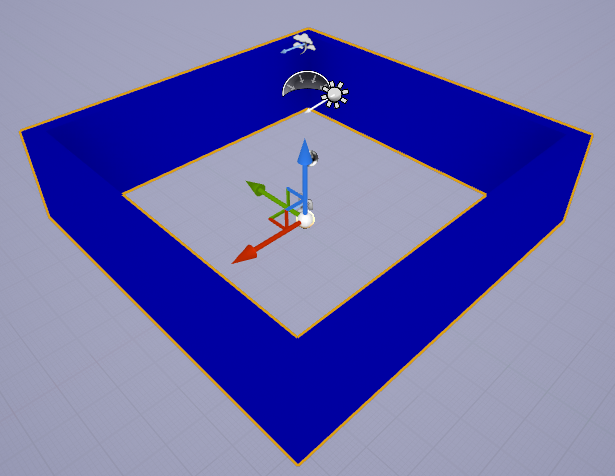
\includegraphics[width=\textwidth]{img/unwrap-method-original-mesh.png}
        \caption{Wall mesh.}
    \end{subfigure}
    \hfill
    \begin{subfigure}[b]{0.48\textwidth}
        \centering
        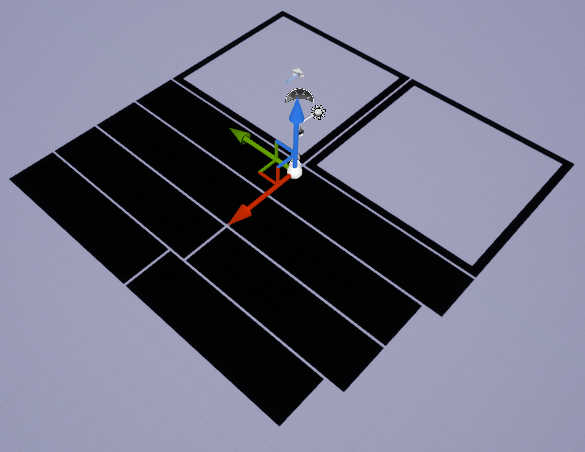
\includegraphics[width=\textwidth]{img/unwrap-method-mesh.png}
        \caption{Unwrapped wall mesh.}
    \end{subfigure}
    \caption{Difference between applied unwrap material.}
    \label{fig:unwrapped-mesh}
\end{figure}

\pagebreak{}
The~result of this algorithm is a~3D vector that is plugged into the~\emph{World Position Offset} pin in Material's result node, which is added to the~total World Position value of a~vertex. The~algorithm consists of creating a~plane in world coordinates from which the~absolute world position is subtracted, so that the~resulting shape is the~desired unwrap plane.

\emph{CaptureSize} parameter specifies the~size of the~square texture in which it will be rendered. For a~2048px texture, a~plane of size $20.48$ metres will appear in the~world, because the~scale of Unreal is in centimetres. This must be set to always add the~correct values to the~texture. 

\emph{UnwrapLocation} vector parameter moves the~centre of the~unwrap plane in the~world. Objects can reside at different locations in the~scene, and hard assigning values to the~scene's origin can cause problems. It may happen that object values are going to be recorded in an~unwrapped state and nothing will be added to the~texture. This is simply caused by the~object having been culled during the~rendering. The~actual position of the~object is somewhere else in the~scene, outside of a~view frustum range.

\begin{figure}[!t]\centering
    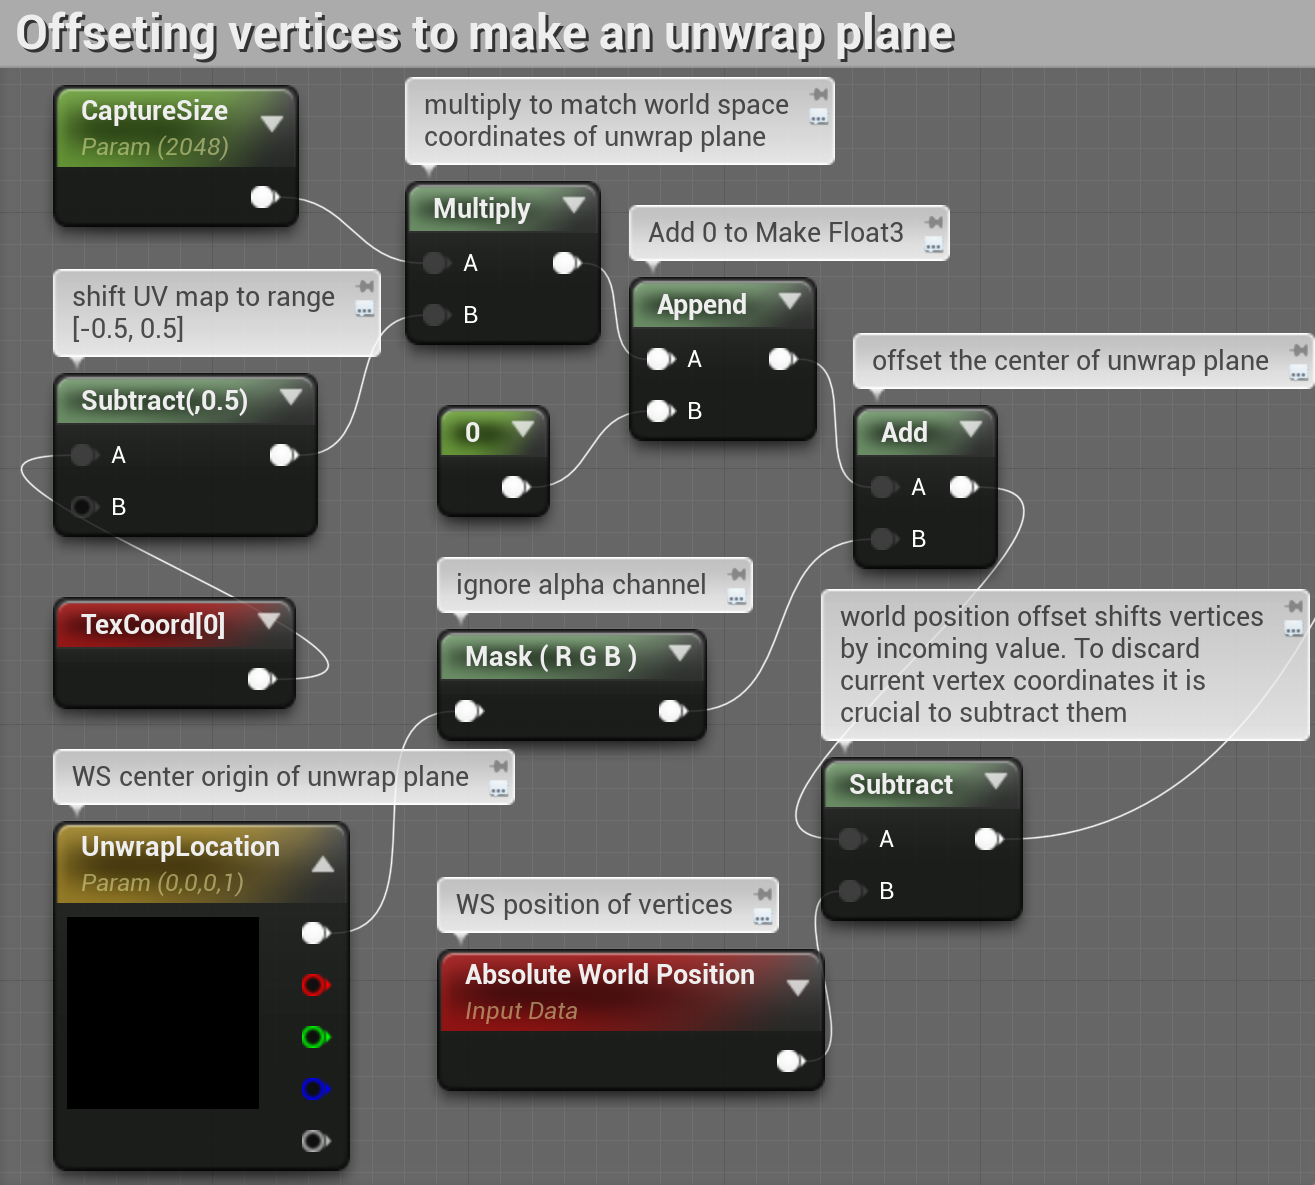
\includegraphics[width=\textwidth]{img/unwrap-method-nodes.png}
    \caption[Material Expressions used to unwrap mesh to world space.]{Material Expressions used to unwrap mesh to world space.~\cite{brucks2016shaderbits}}
    \label{fig:unwrap-offset}
\end{figure}

\pagebreak{}
\subsubsection*{Modification}
Tran proposes a~modification to this method~\cite{tran2018wenderlich} by not storing the~position in an~assistive Render Target, but creating a~3D brush in the~same Material that essentially does the~same thing as the~simpler method. Instead of comparing the~$(u, v)$ coordinate of the~hit location and the~$(u, v)$ coordinate of a~pixel, it compares the~hit location to the~pixel's absolute world position without Material offsets applied. The~implementation can be seen in Figure~\ref{fig:unwrap-3d-brush} which computes the~resulting colour that is supplied to the~Emissive Colour of the~Unwrap Material.

\medskip{}
\emph{BrushSize} parameter specifies the~size of the~3D brush radius. \emph{Strength} parameter determines how hard the~brush imprints on a~texture. It must be in the~range [0, 1]. A~value of 1 would create the~maximum value on the~heatmap and 0 would not make any changes.

\medskip{}
Now the~object is coloured based on a~3D brush that takes into account the~absolute position of the~mesh in the~scene. This method eliminates all the~problems that the~simpler method had.

\medskip{}

Tran's tutorial also offers a~basic Blueprint setup for recording this UV unwrap material using a~Scene Capture Component and a~black projection plane. For more information on the~implementation, see Section~\ref{sec:uv-unwrap-implementation}

\begin{figure}[!ht]\centering
    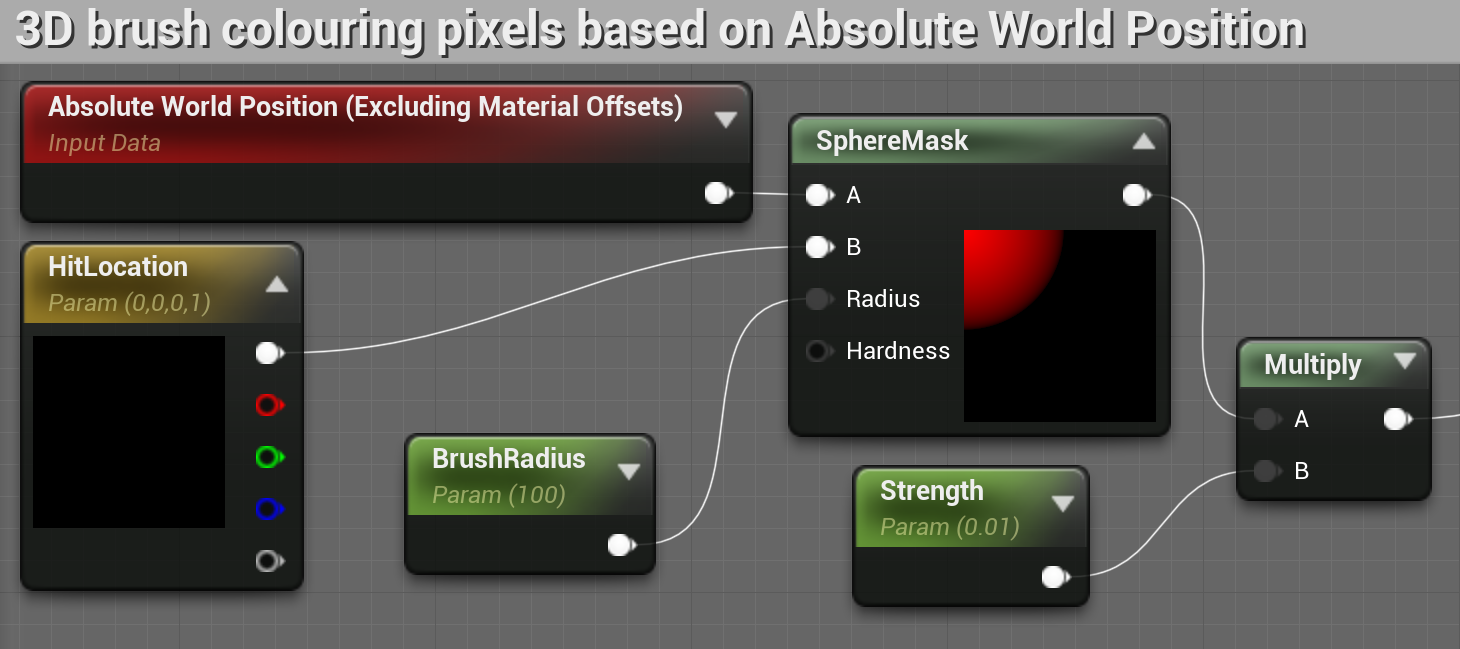
\includegraphics[width=\textwidth]{img/unwrap-method-3d-brush.png}
    \caption{3D Brush defined in Material Expressions.}
    \label{fig:unwrap-3d-brush}
\end{figure}

\subsection{Runtime texture loading}
\label{sec:texture-loading}

Exporting a~Render Target is simple, all it requires is a~single function called \emph{ExportToDisk}. The~function takes a~Texture Object reference, which is the~parent of the~Render Target, a~path with a~filename, and export options. Importing a~texture directly into the~Render Target is more complicated, as no such function exists. It is necessary to obtain the~assistance of a~material shown in Figure~\ref{fig:load-material}. The~process is shown in this tutorial~\cite{texture-loading-tutorial}.

Texture loading options exist, but only as a~Texture 2D object. This is done by the~\emph{Import File as Texture 2D} function, which takes a~file path as input. The~whole method is to redraw the~loaded texture into a~Render Target. Load Material does exactly that; it just sets the~texture parameter itself as the~output colour of the~material. This parameter must be set from the~Dynamic Material Instance by calling its Blueprint function Set Texture Parameter Value -- Figure~\ref{fig:unreal-texture-loading}. The~input value for this function is the~loaded texture, and the~Parameter Name. That must be the~same as the~Param2D name in the~Material.


\begin{figure}[!ht]\centering
    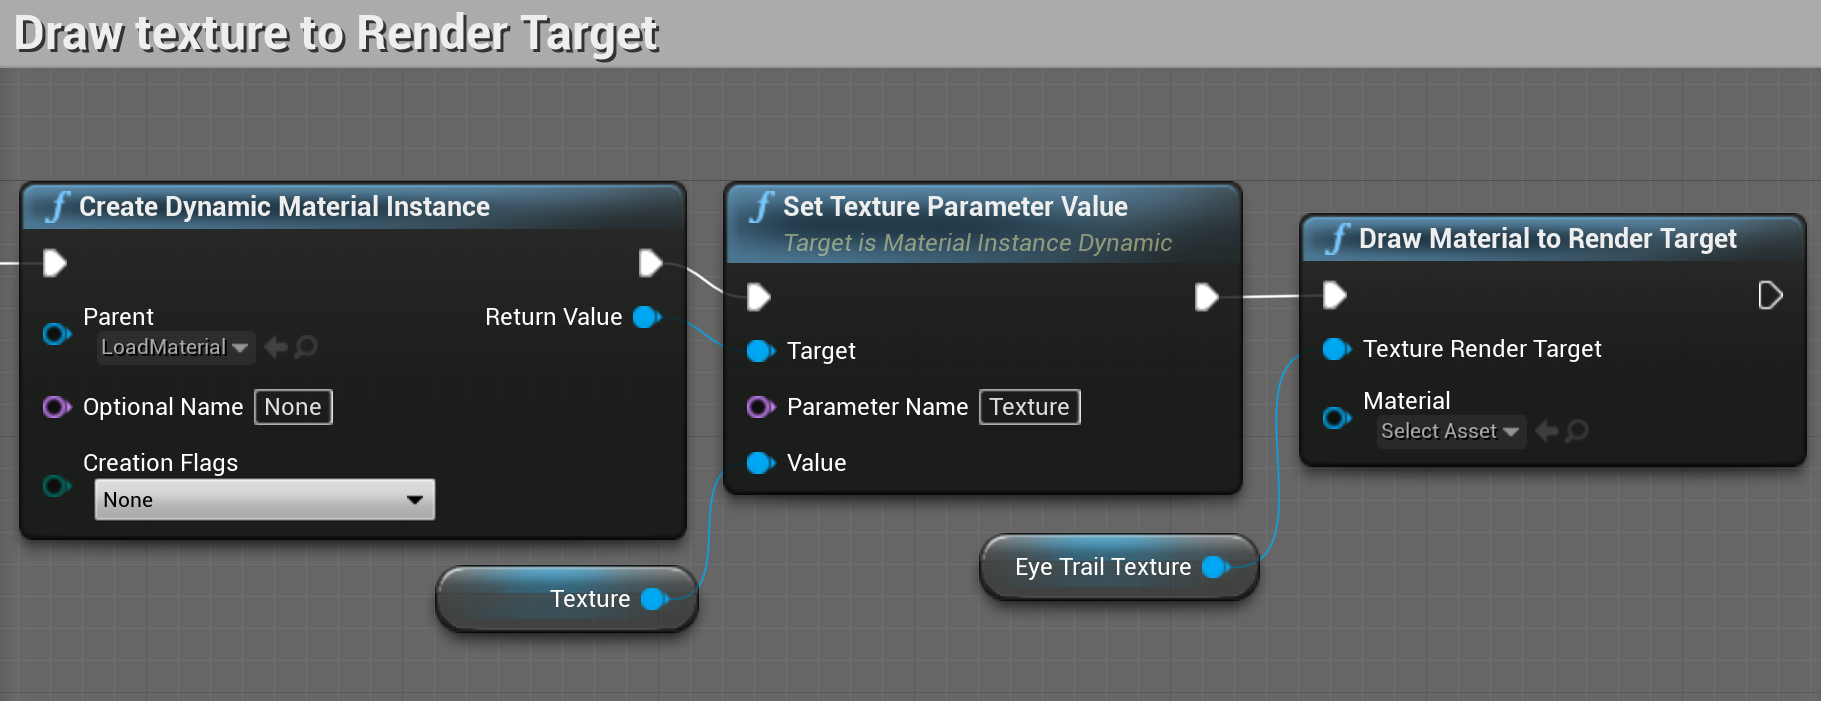
\includegraphics[width=\textwidth]{img/texture-loading.png}
    \caption{Process of importing texture on Render Target.}
    \label{fig:unreal-texture-loading}
\end{figure}

\begin{figure}[!ht]\centering
    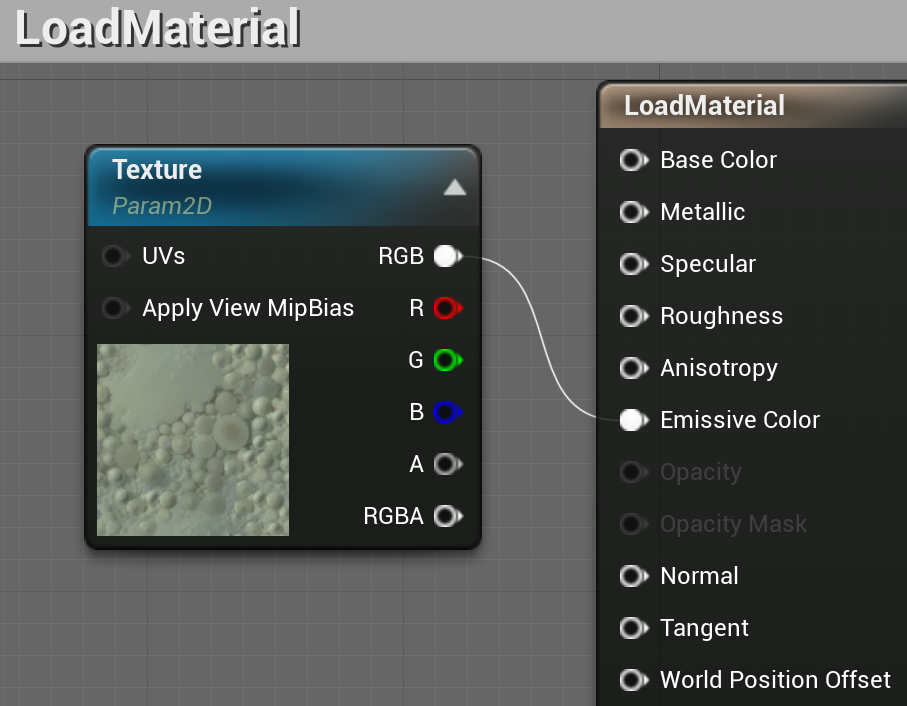
\includegraphics[width=0.8\textwidth]{img/load-material.png}
    \caption[Unreal Material used for loading.]{Unreal Material used for loading.~\cite{texture-loading-tutorial}}
    \label{fig:load-material}
\end{figure}

\chapter{Design}
\begin{chapterabstract}
The~design of the~application prototype is being covered by this chapter. The~form of the~prototype is chosen and a~specific solution is proposed.
\end{chapterabstract}

\section{Requirements}
The~thesis assignment and the~consultations with the~supervisor provide functional and non-functional requirements of the~prototype. 

\subsection{Functional requirements}
Functional requirements define what functionality the~prototype should contain. While creating the~assignment, it was unclear what form it would assume and what methods would be used. 

\begin{description}
    \item[Gaze data collection] The~prototype application should be able to~collect gaze data in some way provided by a~VR HMD with ET.
    \item[Gaze data visualisation] The~prototype shall choose an~appropriate visualisation technique that will be applied to~the~collected gaze data.
    \item[Environment for data collection and visualisation] A~test scene, or experiment, in which gaze data can be visualised and collected from users moving through the~scene.
    \item[Make resultant data] Data are to~be collected from multiple users in a~same environment and combined into resultant data.
\end{description}

\subsection{Non-functional requirements}
Non-functional requirements demand certain qualities and define the~limitations of the~prototype.

\begin{description}
    \item[Technologies] The~main functionalities of the~prototype such as data collection and visualisation, must be developed using a~game engine of choice, Unreal Engine or Unity. Standalone supporting programmes written in \emph{C\texttt{++}} or \emph{Python} can be used to~achieve some of its requirements.
    \item[Documentation] All code must be commented on and described in good detail.
\end{description}

\section{Prototype application}
This section covers the~thought process considering the~situation in which the~prototype was designed, and results in a~decision on what technologies will be used and what form the~prototype application will take.

\subsection{Selected technologies}
\subsubsection*{Software}
An~analysis of current solutions was undertaken -- Section~\ref{sec:solutions} -- to~select the~most appropriate technology to~allow for maximum opportunity to~offer a~new solution. The~Masaryk University thesis dealt with a~similar topic in the~Unity environment. Cognitive3D offers a~very robust, but proprietary, system that uses both engines. Based on this information, this thesis will focus on development in Unreal Engine, as no other open source solution to~this ET problem has been found. Unreal version 4.27 will be used to~develop the~main functionalities of the~prototype. Unreal Engine 5 had not been fully released when this decision was made. During the~writing of the~thesis, this was no longer the~case.

Furthermore, the~Python programming language with the~Pillow library will be used to~create one simple support programme that will process the~collected gaze data.

\subsubsection*{Hardware}
In terms of hardware, there were not many options available and it was generally difficult to~find access to~a~VR headset with ET. There was an~opportunity to~use the~3D~CAVE lab at the~Faculty of Engineering at CTU, which contains an~XTAL headset -- Section~\ref{sec:xtal}. 


Conveniently, there is no solution available that utilises the~ET capabilities of XTAL and, therefore, will be used for this thesis. Furthermore, the~device is of Czech production with local support, and it will be possible to~discuss possible problems and issues with Vrgineers in a~relatively short time.

\subsection{Form}
The~requirement for the~prototype refers to~the~technology used, but does not mention what form it should take. In order to~select the~best form of the~prototype, the~following situation had to~be taken into account.

\subsubsection*{Situation}
The~XTAL headset was chosen for development, but was not physically available for testing at the~time. Based on the~analysis in Section~\ref{sec:xtal}, it operates on its native runtime and it was assumed, due to~the~lack of official data on its ET, that it would return gaze data in the~structure from Section~\ref{sec:gaze-data}. When the~headset became available, it was discovered that this was not true and the~method of data collection had to~be consulted with Vrgineers support, from whom a~beta version of their OpenXR runtime was received. This did not happen until the~later stages of development.

To~avoid unnecessary time loss waiting for the~headset's availability and the~later consultations with support, it was decided to~take the~prototype concept a~bit differently.

\subsubsection*{Proposal}
The~prototype application must be developed without the~access to~a~headset in such a~way that the~collected data from it can be easily used when available. The~task is to~assume that gaze data are available and can be processed, but it is necessary to~provide some alternative to~substitute for their presence. The~forward vector of the~virtual camera inside the~Unreal Engine scene can be used for this purpose.

This made it possible to~think about conceiving the~prototype as an~Unreal Engine \emph{plug-in} that will extend the~functionality of the~game engine or the~Unreal project by the~possibility of collecting and visualising gaze data. The~plug-in will be independent of any~ET hardware and will only require the~origin and direction vector as input.

The~plug-in has the~advantage that it can be mounted on any UE project of the~same version in which it was built. The~assignment needs to~be slightly adjusted to~reflect this change.

\subsection{Modification}

The~plug-in will cover the~functionality of data collection and visualisation, but it still remains to~create an~experiment, the~environment where the~data is collected. The~experiment will be done separately as an~Unreal Engine project, and the~plug-in will be used to~build it. The~plug-in must include functionality that will support the~construction of the~test environment. 

The~practical portion of this thesis is divided into two chapters. The~implementation chapter will present the~implementation of the~plug-in itself, and the~experiment chapter will describe the~construction process of a~test environment using the~plug-in. It will also cover the~use of the~XTAL headset and the~collection of data from multiple users.

The~merging of the~data of multiple participants will not be handled by the~plug-in but rather by a~simple Python script that will be run once after all the~data have been collected.

\section{Functionality}
\label{sec:plugin-functionality}

Based on the~analysis, it was found that all available solutions record the~data first offline and then process them.

This work will focus on a~real time production of heatmaps that can be used both as a~data collection method and as a~data visualisation. Heatmaps will be produced using the~UV unwrap method utilising Unreal Materials as described in Section~\ref{sec:uv-unwrap-method}. Heatmap textures are going to~be loadable and exportable. 

Two heatmaps will be recorded at the~same time. One will typically be created using the~eye gaze, but the~other one will be created based on the~forward vector of a~virtual camera inside the~scene. Both heatmaps will be produced at the~same time for later comparison. This test is intended to~be a~direct demonstration of the~usability of ET. The~collected texture with a~heatmap trail will be displayed on its object using Material. There will be another Material that will directly visualise their mutual appearance.

This thesis will attempt to~implement the~entire prototype using only the~built-in visual programming via Blueprints in Unreal Engine. This is meant to~serve as proof that the~current tools are advanced and that there is really no reason why eye tracking in Unreal Engine should not be pursued by other future projects.

\pagebreak{}

\subsection{Actions}
\label{sec:actions}

When designing a~plug-in, it is worth imagining how an~experiment employing it will look like. The~activity diagram in Figure~\ref{fig:experiment-diagram} describes exactly one of these experiments. It is a~simple one that only initiates, runs, and ends after a~certain amount of time. Once it starts, a~game cycle is triggered that sends two rays into the~scene with each Tick. These, when they collide with an~object that has a~heatmap, will add a~value to~the~heatmap texture.

This leads to~four important actions that the~plug-in must take into account. The~first is the~functionality of shooting rays and processing them. Second, the~colliding ray must recognise if it is an~object that has a~heatmap or if it is an~ordinary scene object. Third, imprinting a~value on one of the~object's textures. The~object will have two of those, so the~colliding ray classification needs to~be added. And finally, export all heatmaps.

\subsubsection*{Eye Tracked object}

This is an~object that will be modifiable with this plug-in. It must be defined as such to~be affected by a~ray. In the~context of the~Unreal Engine, it should be a~Component or an~Actor that has direct access to~static mesh data.

During the~creation of an~experiment, the~desired functionality is that it should be sufficient to~insert this type of object into the~scene, not worry about much else, and be assured that a~ray will collide with it. As part of the~plug-in design, this object can also be used for possible subsequent iterations for other ways of visualising or collecting data.

The~object will contain an~export function that saves both textures to~a~local drive. In order to~save all these textures of all objects, a~static function will have to~be defined to~iterate through all the~Eye Tracked objects in the~scene and use their respective export function.

\subsubsection*{Raycaster}

This object will be responsible for sending rays into the~scene based on the~input of the~origin and direction vector. Within a~test scene, these rays should be emitted from a~defined Pawn or Character that is used to~navigate through the~scene. It is logical to~use the~collision function from this perspective so that the~function itself does not use this Actor during collision calculations. If an~Actor unrelated to~the~emitted ray were used for these, the~collision would never reach the~world because it could be trapped inside a~collision volume of the~Actor, which would be part of the~collision calculations, unless excluded.

One could certainly create such a~Pawn within a~plug-in and hard-code the~raycasting capabilities into it, but this is not a~solution that is extensible, as each scene may require different scene traversal logic and functionalities.

Therefore, raycasting must be implemented within a~Component that can then be added to~any Pawn or Character.

\subsubsection*{Heatmap renderer}

The~heatmap rendering method will be adopted from this article~\cite{tran2018wenderlich} with a~static mesh UV unwrap Material defined in Section~\ref{sec:uv-unwrap-method}. The~entire rendering depends on an~Actor that must be in the~scene. This Actor has to~contain a~black projection plane placed on the~floor of the~scene that is the~size of the~unwrapped mesh, i.e. for a~1024x1024px texture, a~square plane with an~edge length of 100 cm has to~be scaled 10.24 times. The~plane creates a~black background so that the~renderer avoids parasitic surrounding effects.

The~Component that will capture this is the~Scene Capture Component, which will have a~defined Show-Only List that will contain only the~rendered object with a~black background; only those two will be rendered. It must be rendered in orthographic mode, where its view width must be equal to~the~width of the~texture that will be modified.
\pagebreak{}

\begin{figure}[p]\centering{}
    \includesvg[width=\textwidth]{img/experiment-diagram.svg}
    \caption{Activity diagram of a~possible ET experiment collecting heatmaps.}
    \label{fig:experiment-diagram}
\end{figure}
\chapter{Implementation}
\label{chap:implementation}
\begin{chapterabstract}
The~implementation of the~EyeTrackingUtilities plug-in is described in this chapter. When added to an~Unreal Engine project, it offers a~Blueprint and Material directory in its Content folder. The~project can immediately use its contents.
\end{chapterabstract}

\section{Materials}

Materials are key to the~functionality of visualisation and collection of heatmaps. All of them will be described in this section. Material Content folder can be seen in Figure~\ref{fig:material-folder}.

\begin{figure}[!ht]\centering
    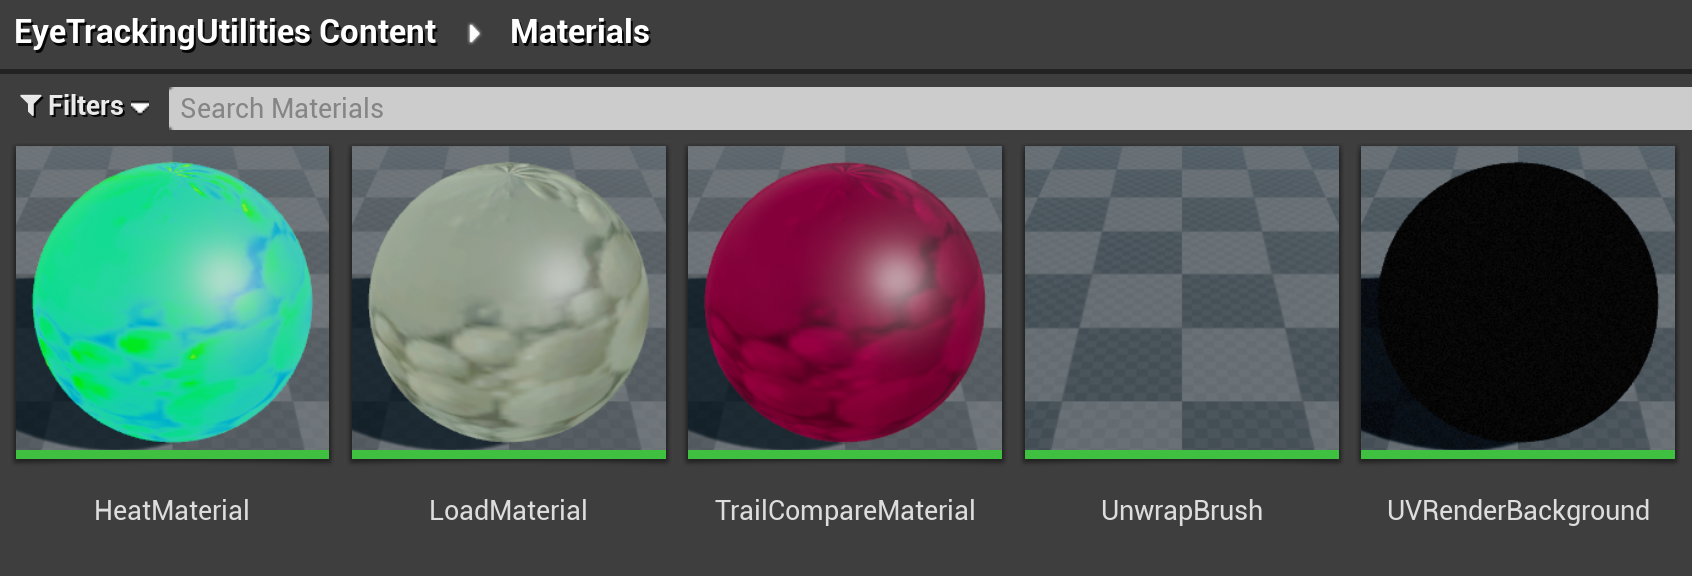
\includegraphics[width=\textwidth]{img/plugin-materials.png}
    \caption{Contents of EyeTrackingUtilities Material folder.}
    \label{fig:material-folder}
\end{figure}

\subsection{LoadMaterial and UVRenderBackground}
These are the~two simplest materials. \emph{UVRenderBackground} is a~material that constantly assigns a~black colour -- a~value of (0, 0, 0) -- to the~base colour, metallic, and specular pins of its result node.

\emph{LoadMaterial} is exactly the~same Material described in Section~\ref{sec:texture-loading}, to load already exported heatmap textures.
\pagebreak{}

\subsection{UnwrapBrush}
\label{sec:unwrap-brush-implementation}

\emph{UnwrapBrush} is an~implemented version of the~Material from Section~\ref{sec:uv-unwrap-method} using Tran's modification to skip several rendering steps using a~3D brush. The~block of material expressions in Figure~\ref{fig:unwrap-offset} is connected to the~World Position Offset pin of the~resulting Material node, and another part in Figure~\ref{fig:unwrap-3d-brush} is connected to Emissive Colour pin.

This technique enables rendering heatmap textures on a~GPU, so the~computation is very fast and does not slow down the~overall performance even when rendering 2K textures. However, it does have one problem, which is related to the~use of a~3D brush. If the~brush is large enough or even larger than the~object itself, it paints the~parts of the~object that are not visible. An~illustrative video demonstration is available in the~enclosed media in \path{video/02-3D-brush-problem.mp4}.

This problem was solved by adding two parameters related to a~collision in the~scene. The~solution can be seen in Figure 4.2.

\subsubsection*{HitNormal parameter}
\emph{HitNormal} is the~normal of the~static mesh at the~collision point in world coordinates. The~reason to use this is so that one can determine which pixel to colour based on the~size of an~angle between the~normal of a~currently drawn pixel in world coordinates and the~normal of the~collision point. This is to prevent the~brush from drawing on faces with an~opposite normal; those that are at an~obtuse angle to the~collision point.

When this angle is greater than $92{^\circ}$, the~pixel is assigned a~black colour. A~$90{^\circ}$ could have been used, but that would have prohibited the~simultaneous drawing on two perpendicular faces, which is desirable in some situations because both faces can be viewed at $45{^\circ}$.

But that does not solve the~whole problem because it is calculated only from the~object's perspective. It is still possible to draw on surfaces perpendicular to those on which the~collisions occur, even though they are not visible from the~camera view. 

\subsubsection*{DirectionToCamera parameter}
The~\emph{DirectionToCamera} parameter handles just that. The~method is exactly the~same as for the~previous parameter, but a~different threshold is set. It takes a~direction vector to the~camera and a~normal of the~pixel in the~WS. It will draw on all surfaces as long as the~camera is looking at them at $88{^\circ}$.

Note that using both of these angular conditions simultaneously will sometimes not guarantee drawing on a~face that is visible but not colliding with a~ray. The~former condition will guarantee that one can draw only on one of the~two faces that form an~acute-angle edge. At the~same time, however, it is not enough to use only the~latter condition, because sometimes the~brush may bleed through to the~other side of narrow objects and acute angles of the~camera.

\subsection{HeatMaterial}
\label{sec:heat-material-implementation}

Basic Material that visualises a~heatmap texture on a~mesh. Composed of four colours that are interpolated by the~value of one texture channel, as shown in Figure~\ref{fig:heatmap-material}~\cite{basic-heatmap-tutorial}. The~result is projected as the~colour of the~mesh. A~heatmap texture is added using the~texture parameter \emph{HeatTrail}. 

\pagebreak{}

\begin{figure}[!htb]\centering
    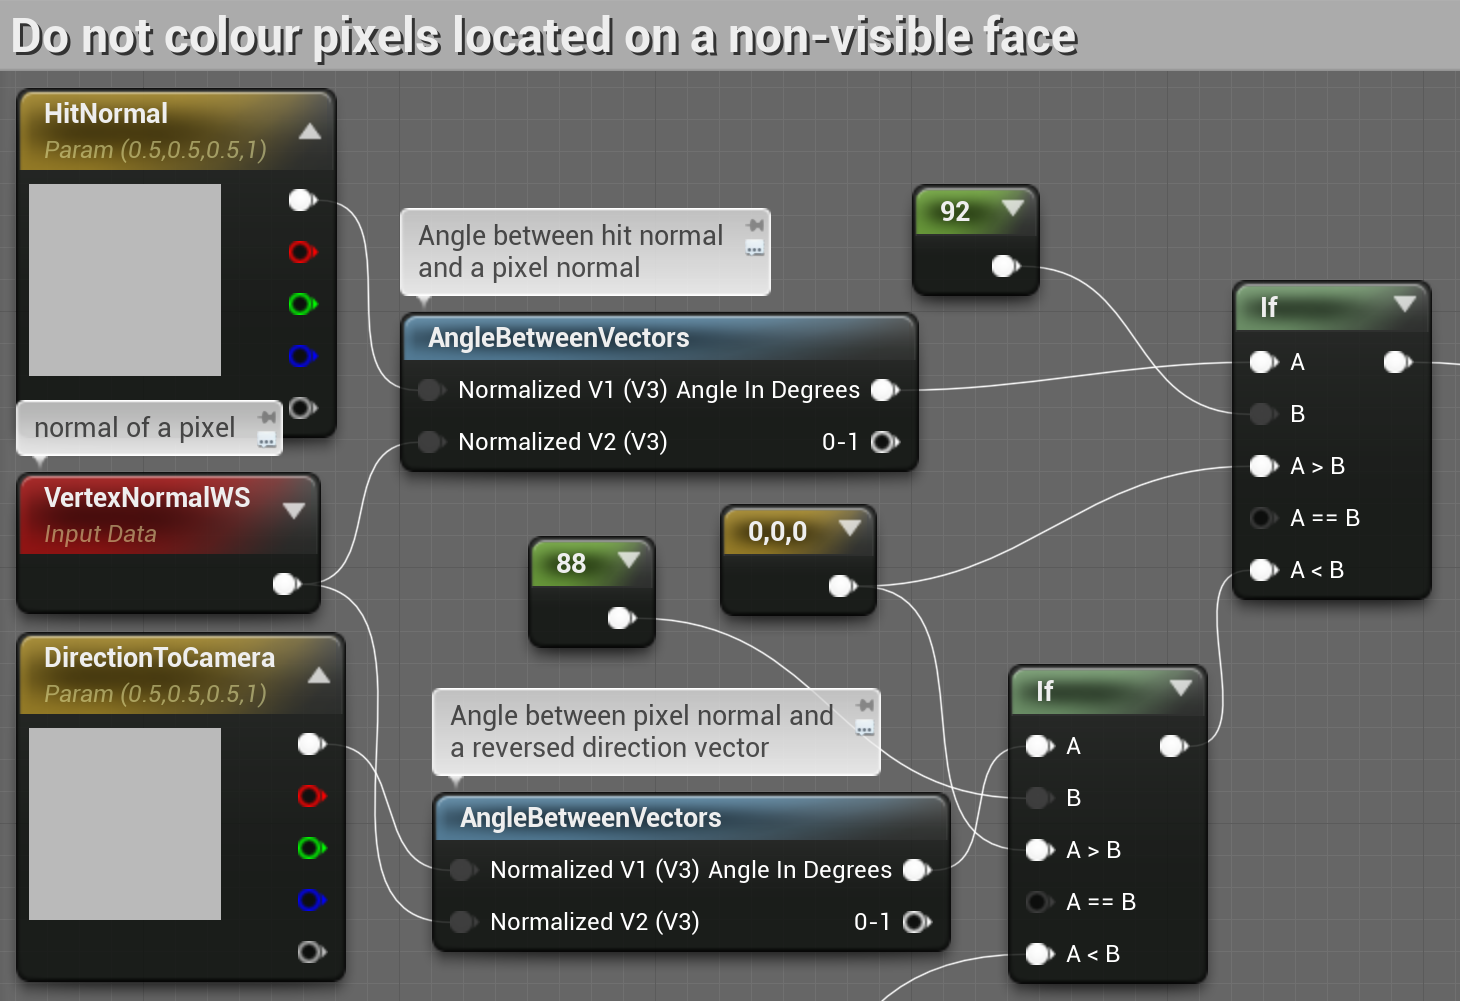
\includegraphics[width=\textwidth]{img/unwrap-brush-correction.png}
    \caption{Unwrap 3D brush material correction with angular conditions.}
    \label{fig:unwrap-brush-correction}
\end{figure}

\begin{figure}[!htb]\centering
    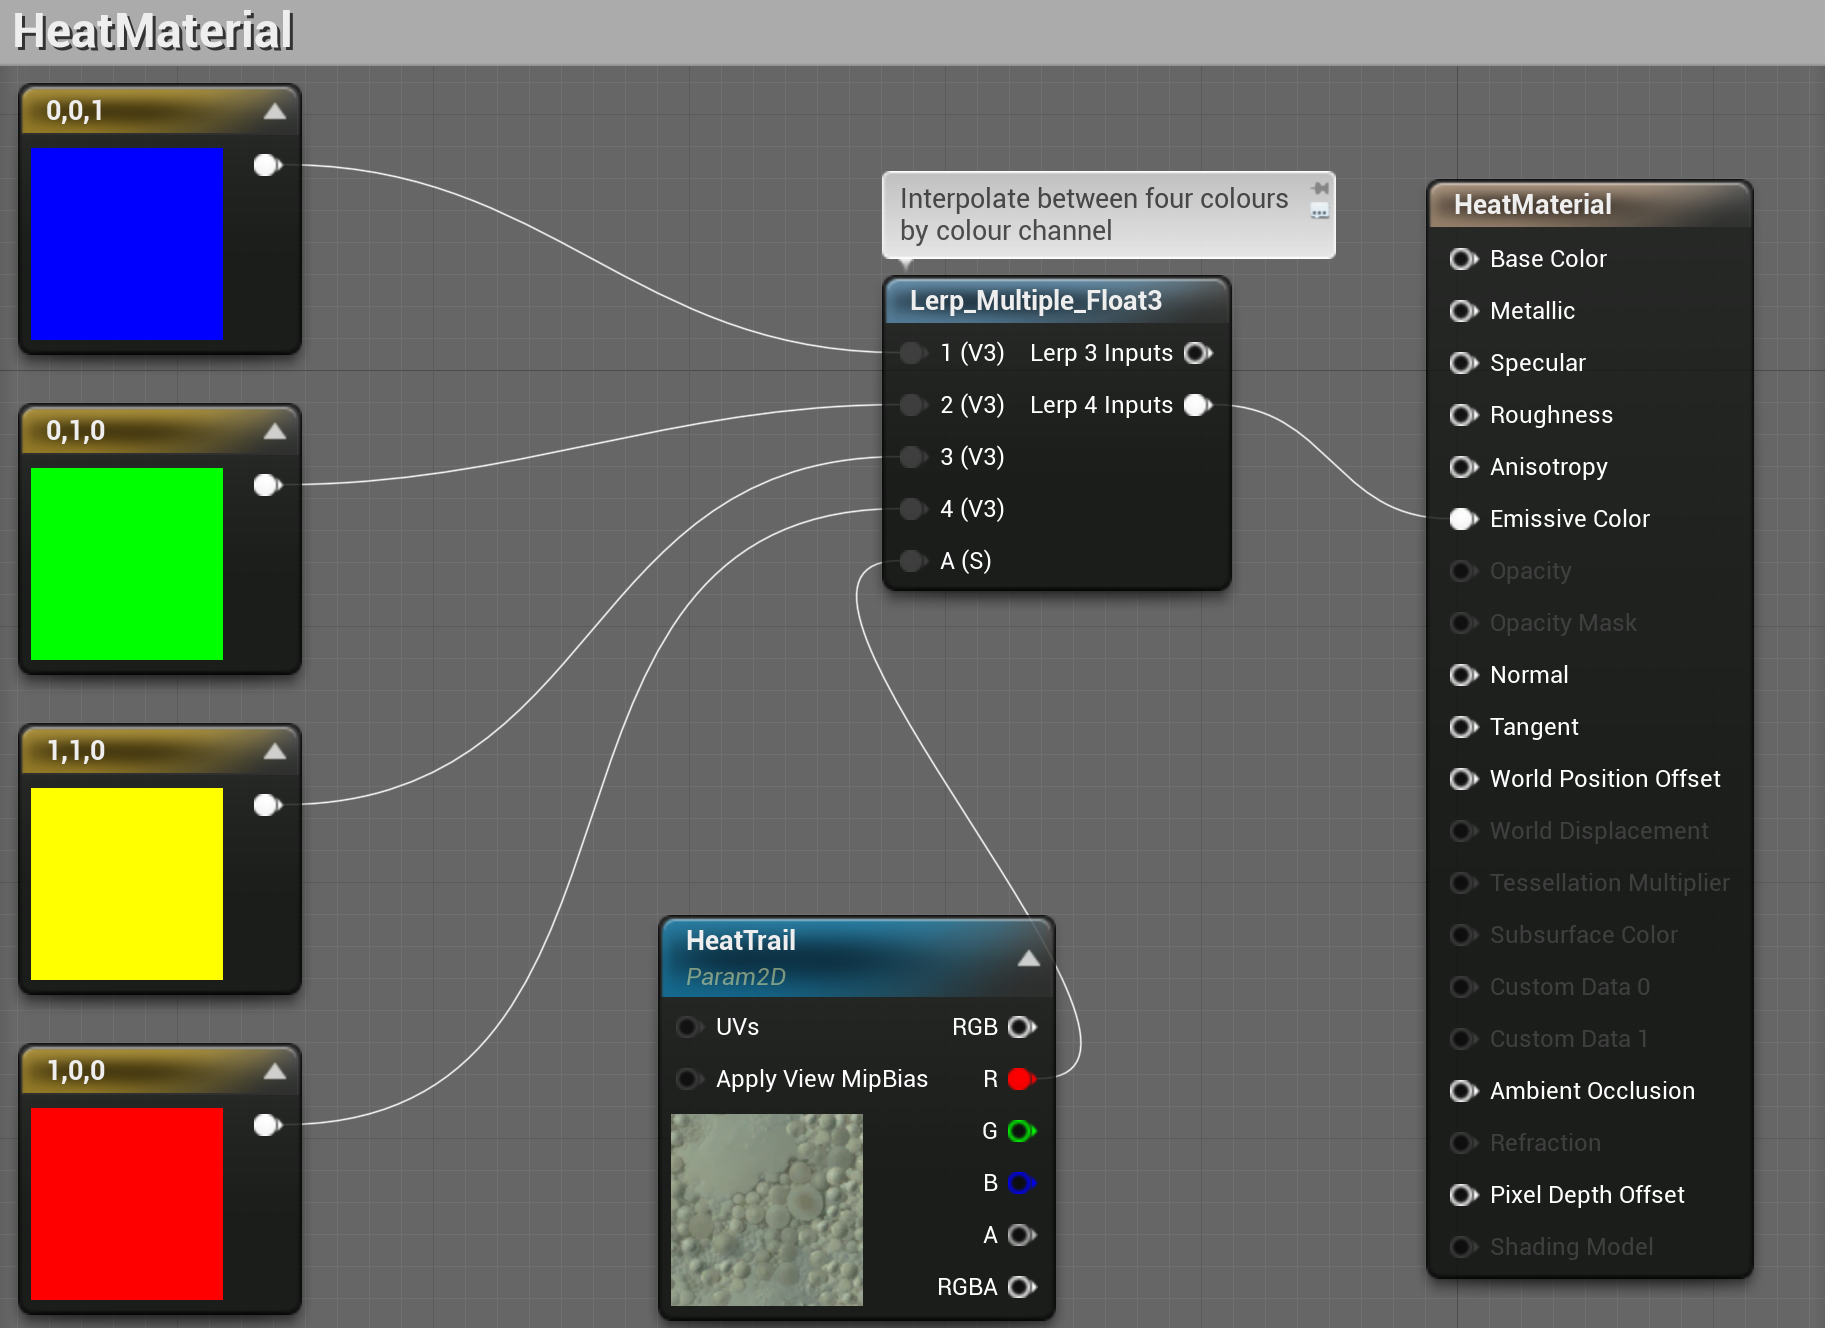
\includegraphics[width=0.85\textwidth]{img/heat-material.png}
    \caption{HeatMaterial node definition.}
    \label{fig:heatmap-material}
\end{figure}


\subsection{TrailCompareMaterial}
\label{sec:trail-compare-implementation}

Simple material that combines two colours into one to visualise the~appearance of two different textures on an~object with a~heatmap. The~definition is described in Figure~\ref{fig:trail-compare}.

\begin{figure}[!ht]\centering
    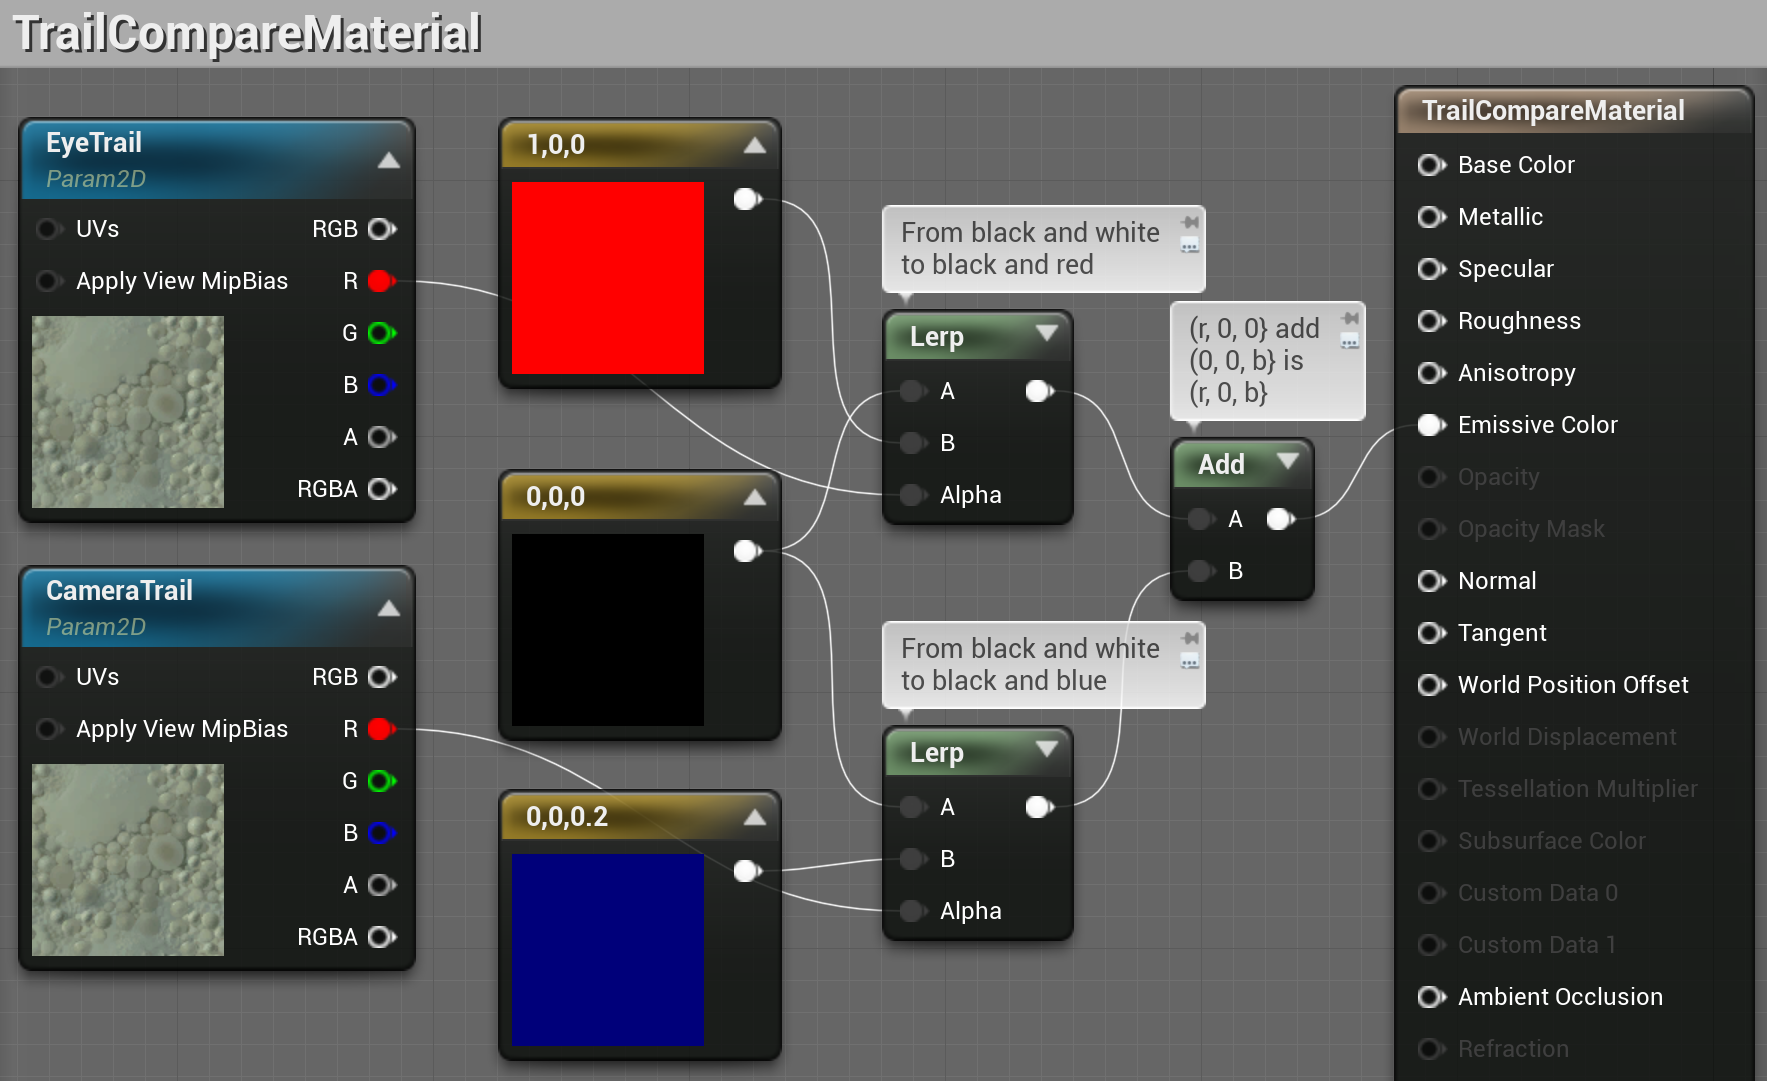
\includegraphics[width=\textwidth]{img/trail-compare-material.png}
    \caption{TrailCompareMaterial node definition.}
    \label{fig:trail-compare}
\end{figure}

\section{Blueprints}

This section presents the~implementation of classes with functionalities designed in Section~\ref{sec:plugin-functionality}. Contents of the~plug-in's Blueprint folder is in Figure~\ref{fig:blueprint-folder} 

\begin{figure}[!ht]\centering
    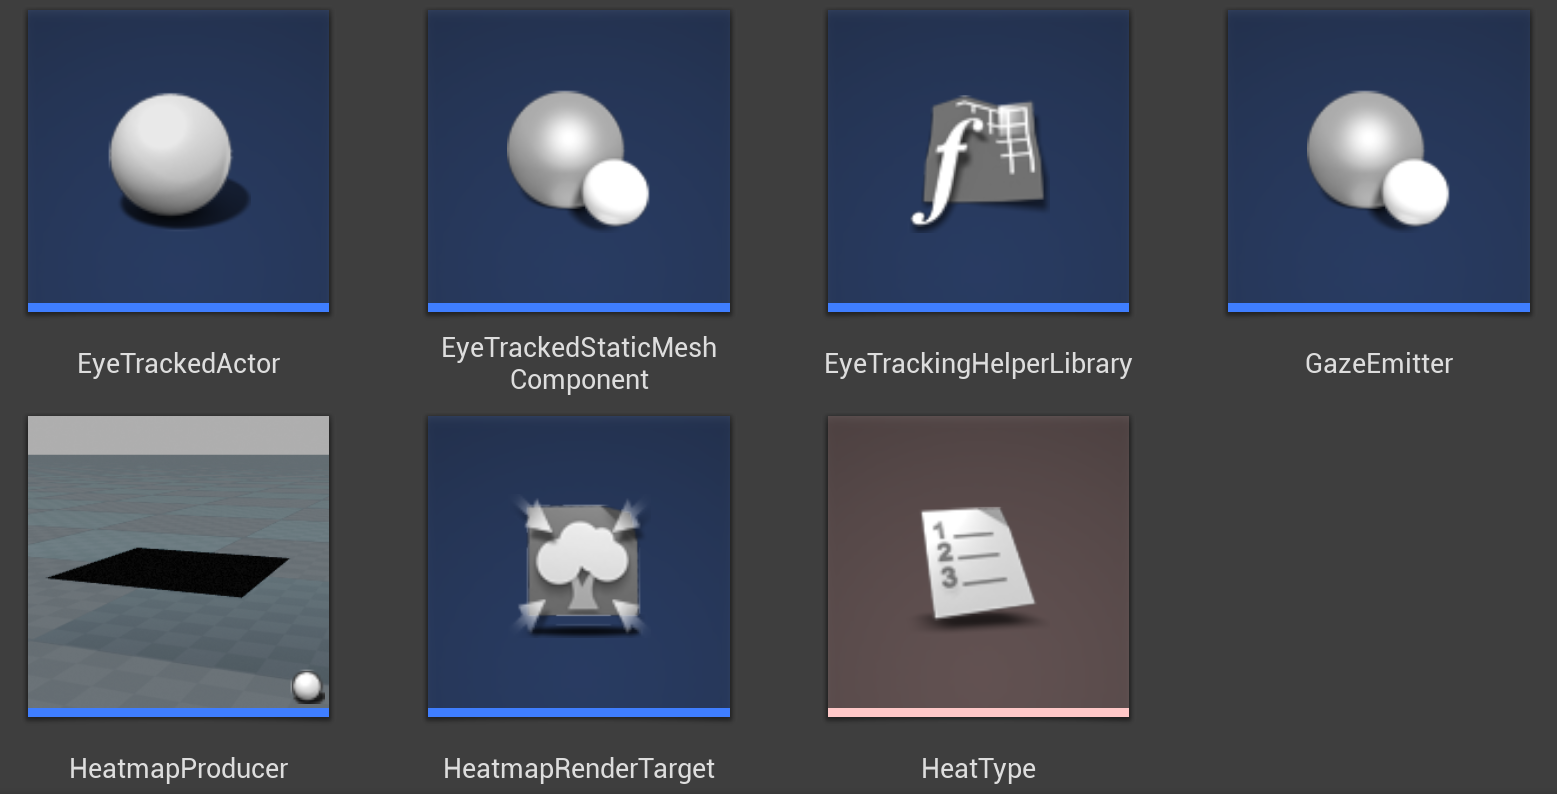
\includegraphics[width=0.8\textwidth]{img/plugin-blueprints.png}
    \caption{Contents of EyeTrackingUtilities Blueprint folder.}
    \label{fig:blueprint-folder}
\end{figure}

\subsection{EyeTrackedStaticMeshComponent}
\label{sec:static-mesh-ET}

\emph{EyeTrackedStaticComponent} is a~component inherited from \emph{StaticMeshComponent}. This class extends the~original static mesh functionality with two private render targets; \emph{EyeTrailTexture}, \emph{CameraTrailTexture}; and two private material instances; \emph{HeatmapMaterial}, \emph{CompareTrailMaterial}.

Both render targets have an~adjustable resolution in one variable that is initiated once when the~application starts. One is enough, because the~render targets must be a~square. Furthermore, it can be decided that a~given component can be EyeTracked but does not have to have its own heatmap, so a~public boolean \emph{AcceptsHeat} property was added.

The~render target is initialised by calling a~single Blueprint function called Create Canvas Render Target 2D, which is given a~width and height. This is done twice in total, as illustrated in Figure~\ref{fig:RT-init}. Furthermore, both instances of dynamic materials are initialised. Blueprint nodes of this operation can be seen in Appendix~\ref{appendix:ETcomponent}.

Render targets are private variables. To use them for rendering, a~Scene Capture Component from other classes will have targets assigned within this class. The~function \emph{AttachRenderer} in Figure~\ref{fig:attach-renderer} serves this purpouse.

\begin{figure}[!ht]\centering
    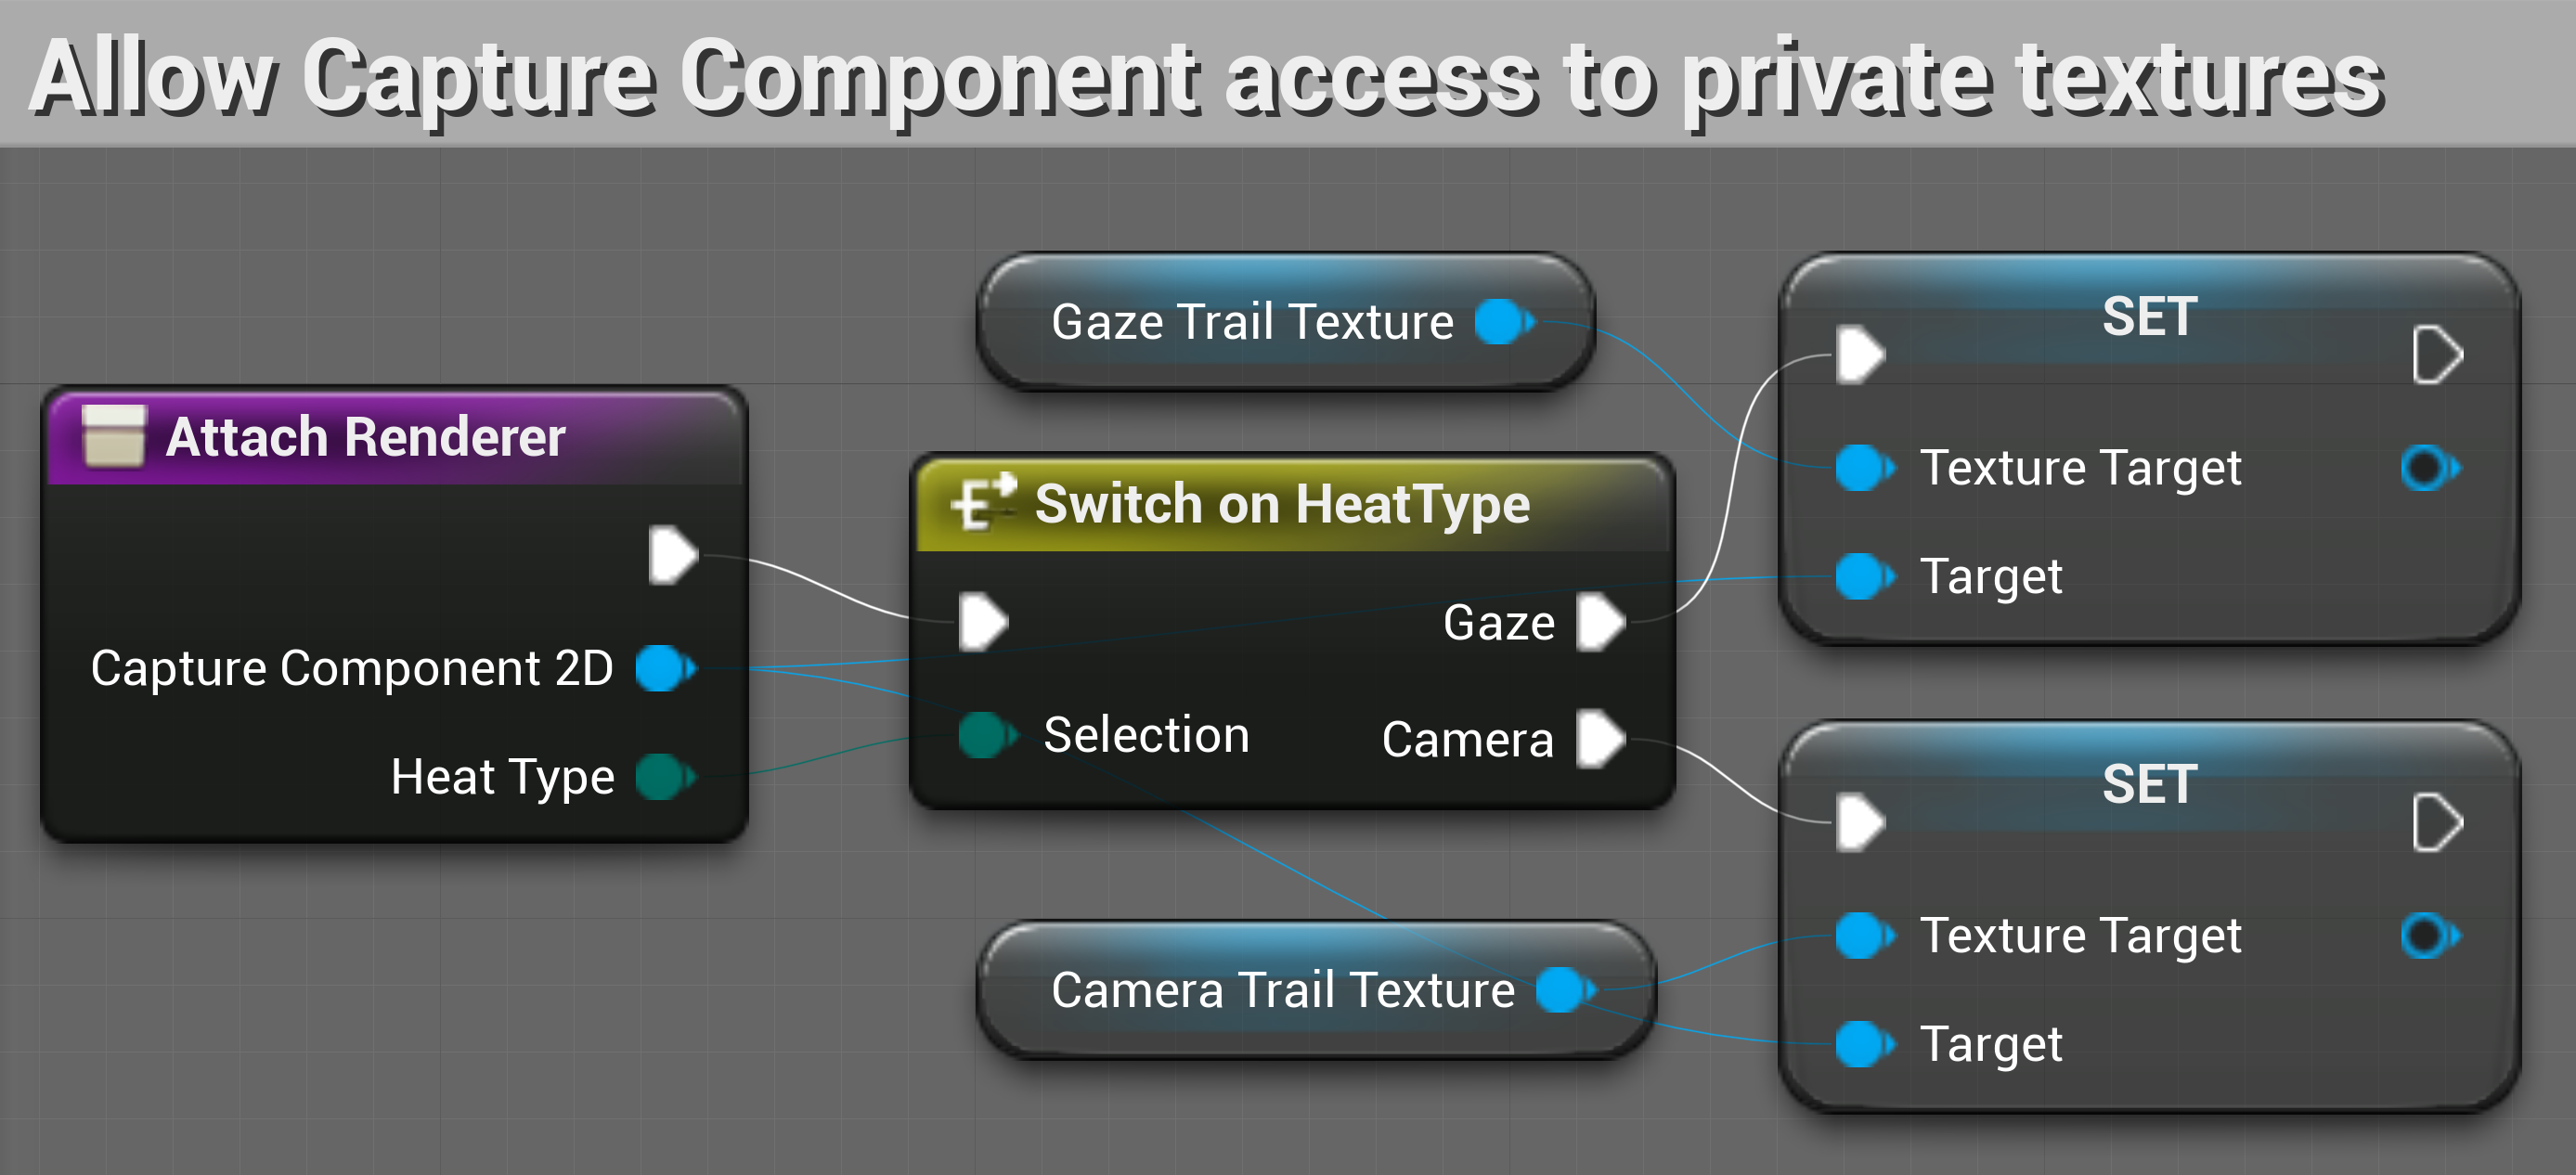
\includegraphics[width=0.6\textwidth]{img/attach-renderer.png}
    \caption{AttachRenderer function in EyeTrackedStaticMeshComponent.}
    \label{fig:attach-renderer}
\end{figure}

\begin{figure}[!ht]
    \centering
    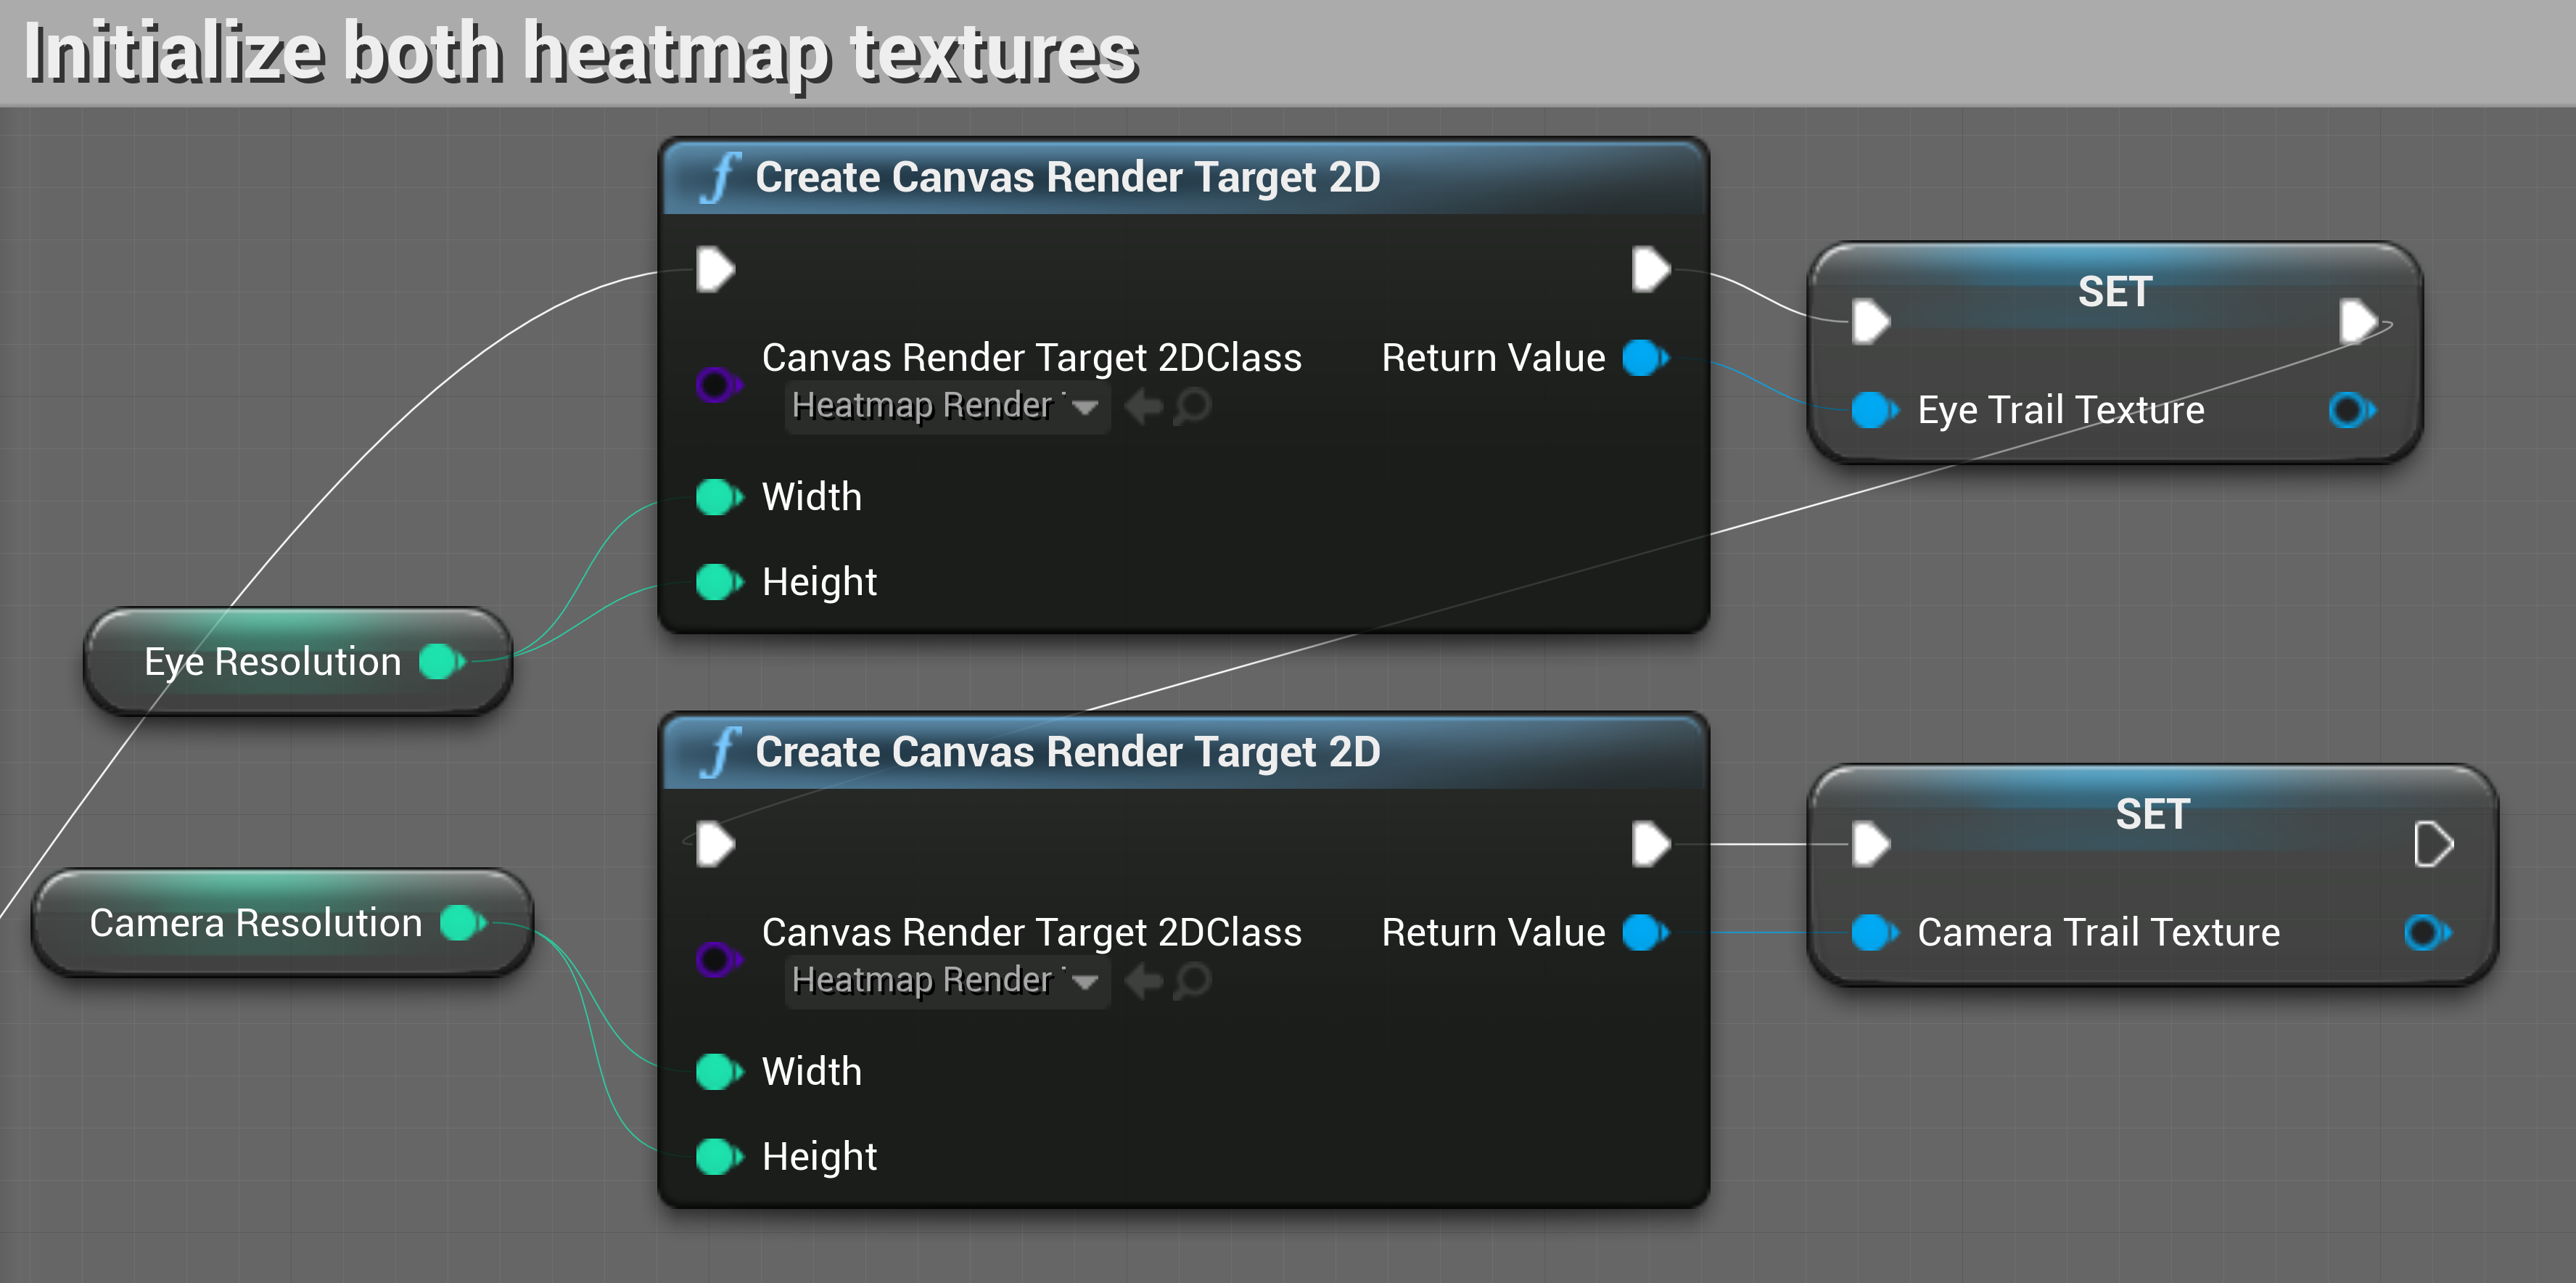
\includegraphics[width=\textwidth]{img/ETcomponent-init.png}
    \caption{EyeTrackedStaticMeshComponent render target initialisation.}
    \label{fig:RT-init}
\end{figure}

\pagebreak{}

\subsubsection*{Texture file operations}
Another key function of this component is the~export and import of heatmap textures. The~format is RGBA with 16-bit colour depth for higher accuracy of the~measured heatmaps. For this type of texture, the~EXR format was chosen. Unreal Engine offers disk input and output operations in this format. The~reason for choosing it was that EXR-format images can be exported and imported using the~OpenEXR library for Python~\cite{openexr}, which will be useful for later image processing.

The~whole export depends only on creating a~file path and calling the~\emph{ExportToDisk} Blueprint function, which takes the~export options as a~pin. There, it is possible to choose the~texture export format and the~compression rate; Figure~\ref{fig:export-heatmaps-exr}. The~path to the~file is created by simple string operations shown in Figure~\ref{fig:make-filepath}. The~comment of these nodes also contains the~format of the~path that the~operations create. In total, two paths are created. One for the~gaze heatmap and one for the~camera heatmap.

The~loading depends first on loading the~image file itself by calling the~\emph{Import File as Texture2D} function and passing the~filename parameter. 
The~procedure for passing this texture object to an~editable render target can be seen in Figure~\ref{fig:load-heatmap-textures}. A~new dynamic material instance of LoadMaterial is created. This material is given a~texture parameter with the~value of the~loaded texture object to be rendered by the~\emph{Draw Material To Render Target} function.

\subsubsection*{EyeTrackingHelperLibrary}

This is a~static library with Load, Export, and Toggle functions that take care of iterating through all EyeTrackedStaticMeshComponents in the~scene and then calling their respective functions individually.

\begin{figure}[!ht]
    \centering
    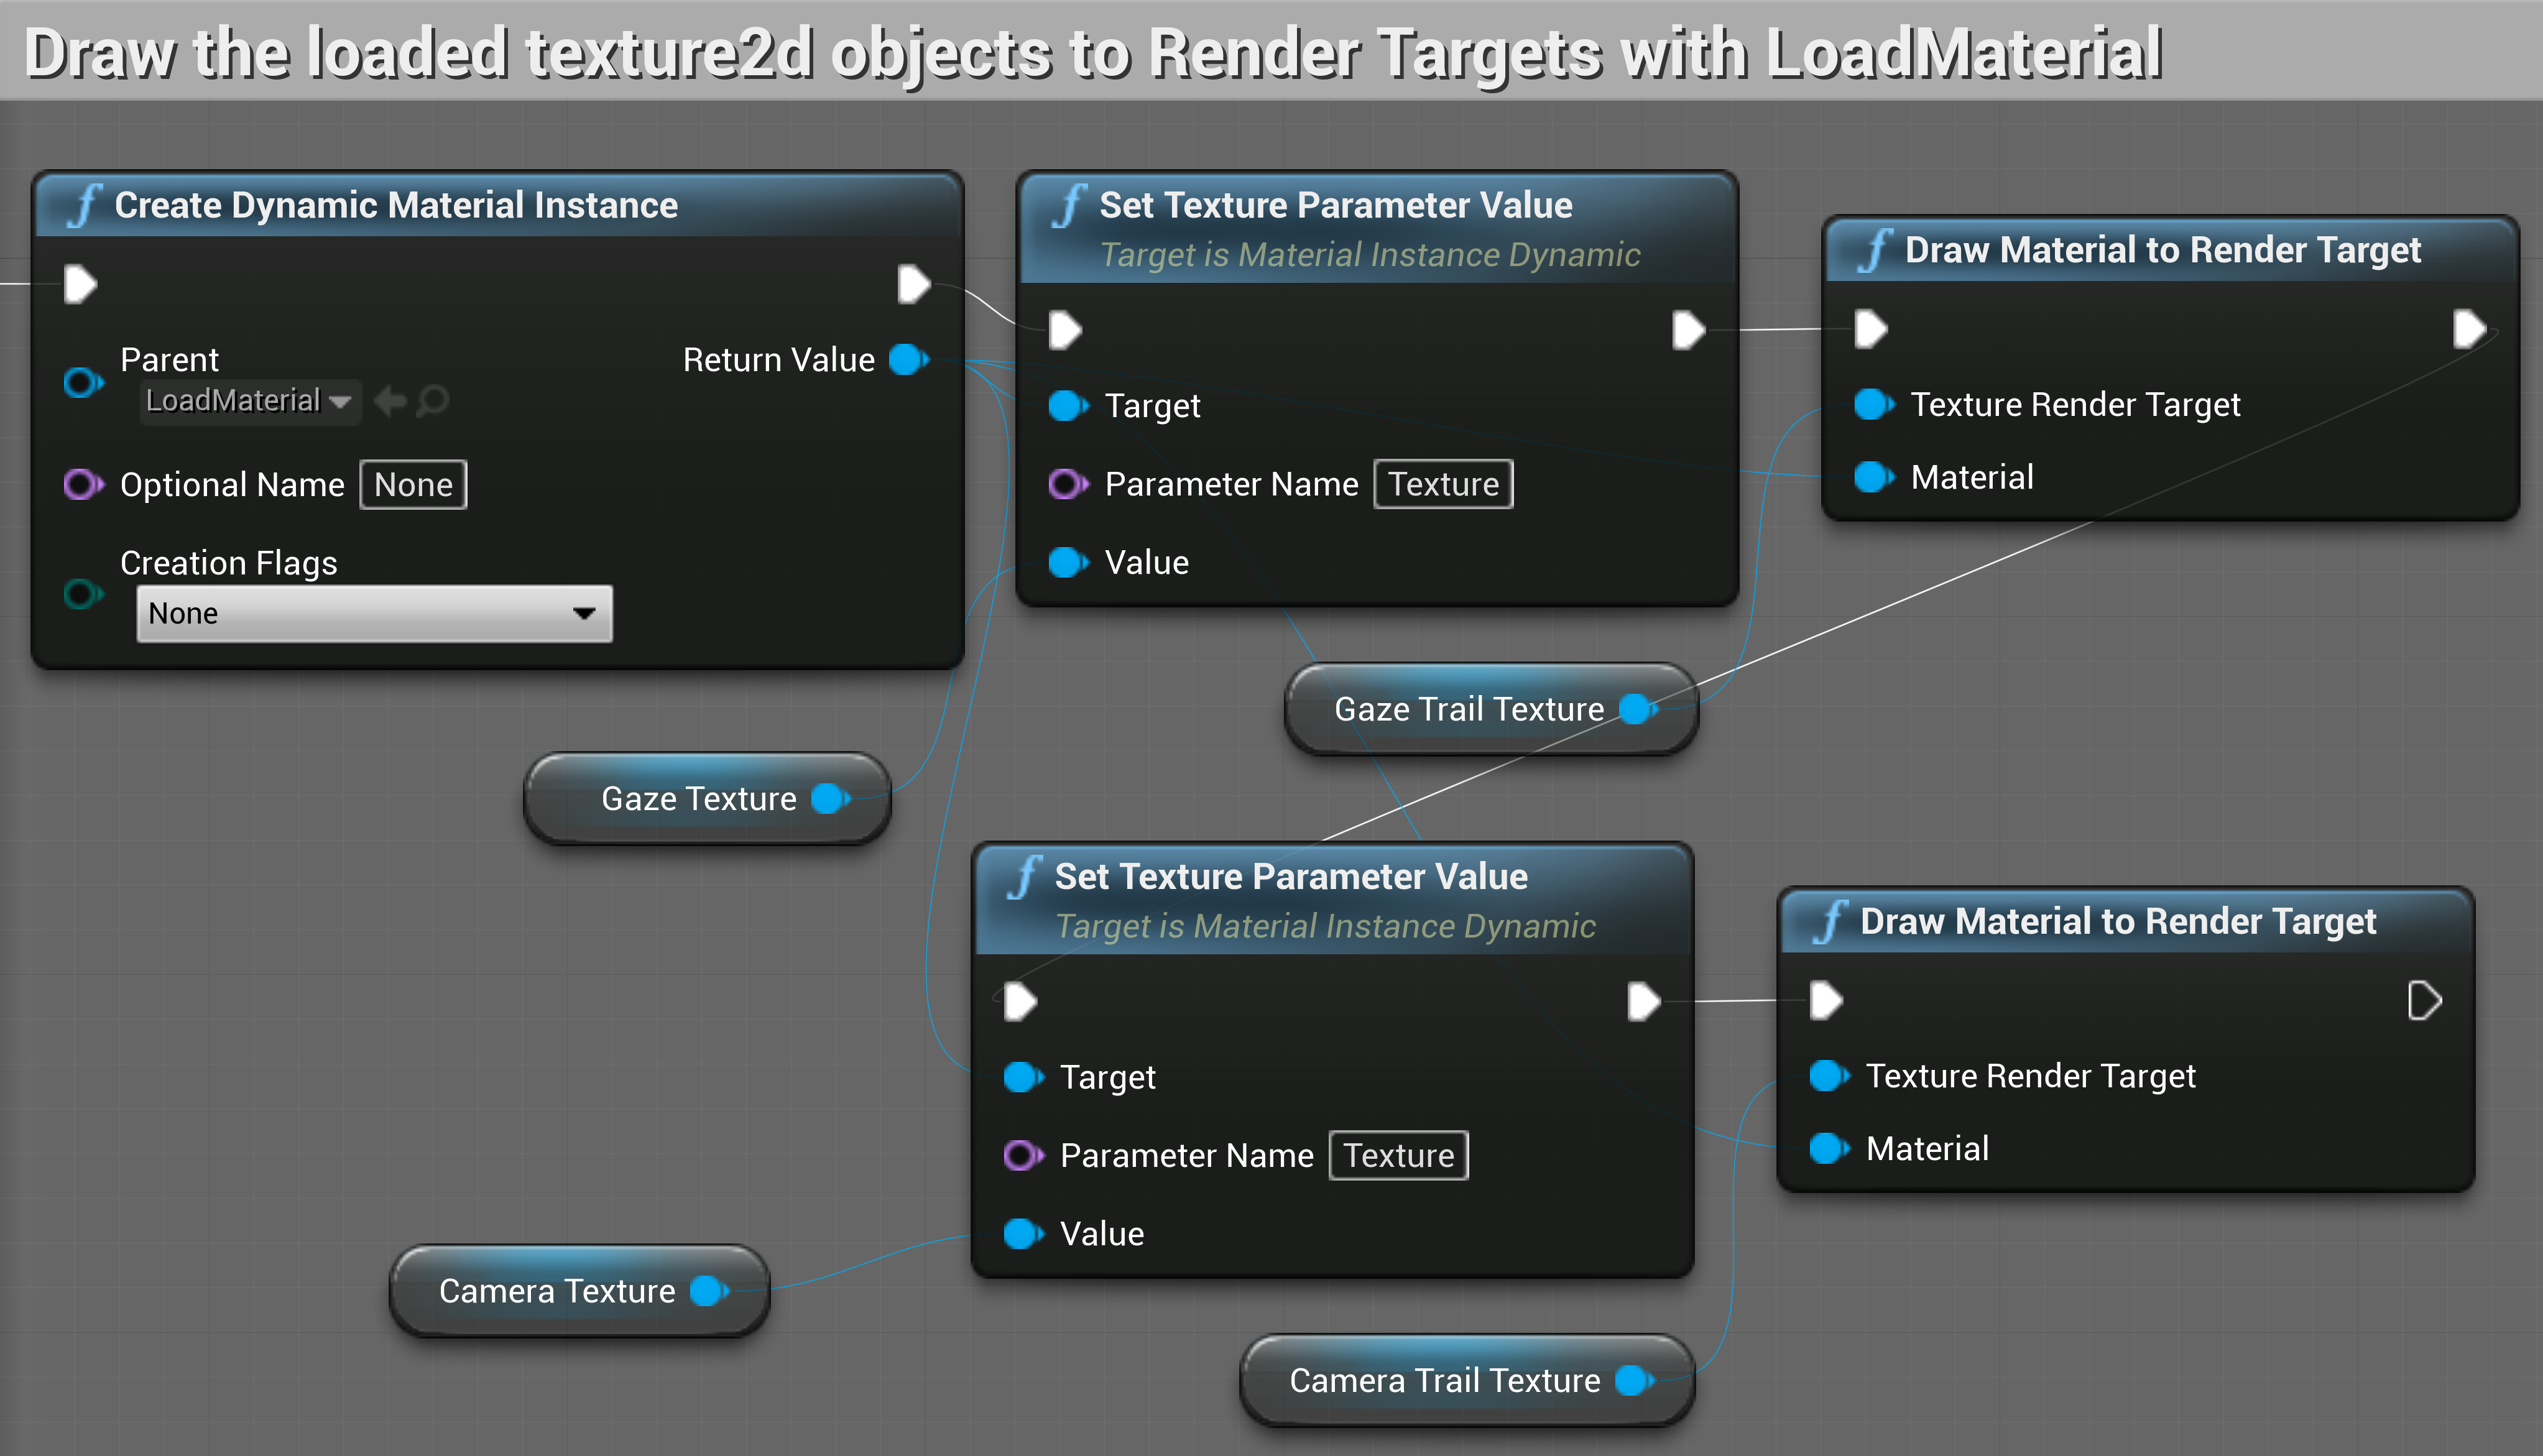
\includegraphics[width=\textwidth]{img/load-heatmap-textures.png}
    \caption{Loading heatmap textures to render targets.}
    \label{fig:load-heatmap-textures}
\end{figure}

\pagebreak{}

\begin{figure}[!ht]
    \centering
    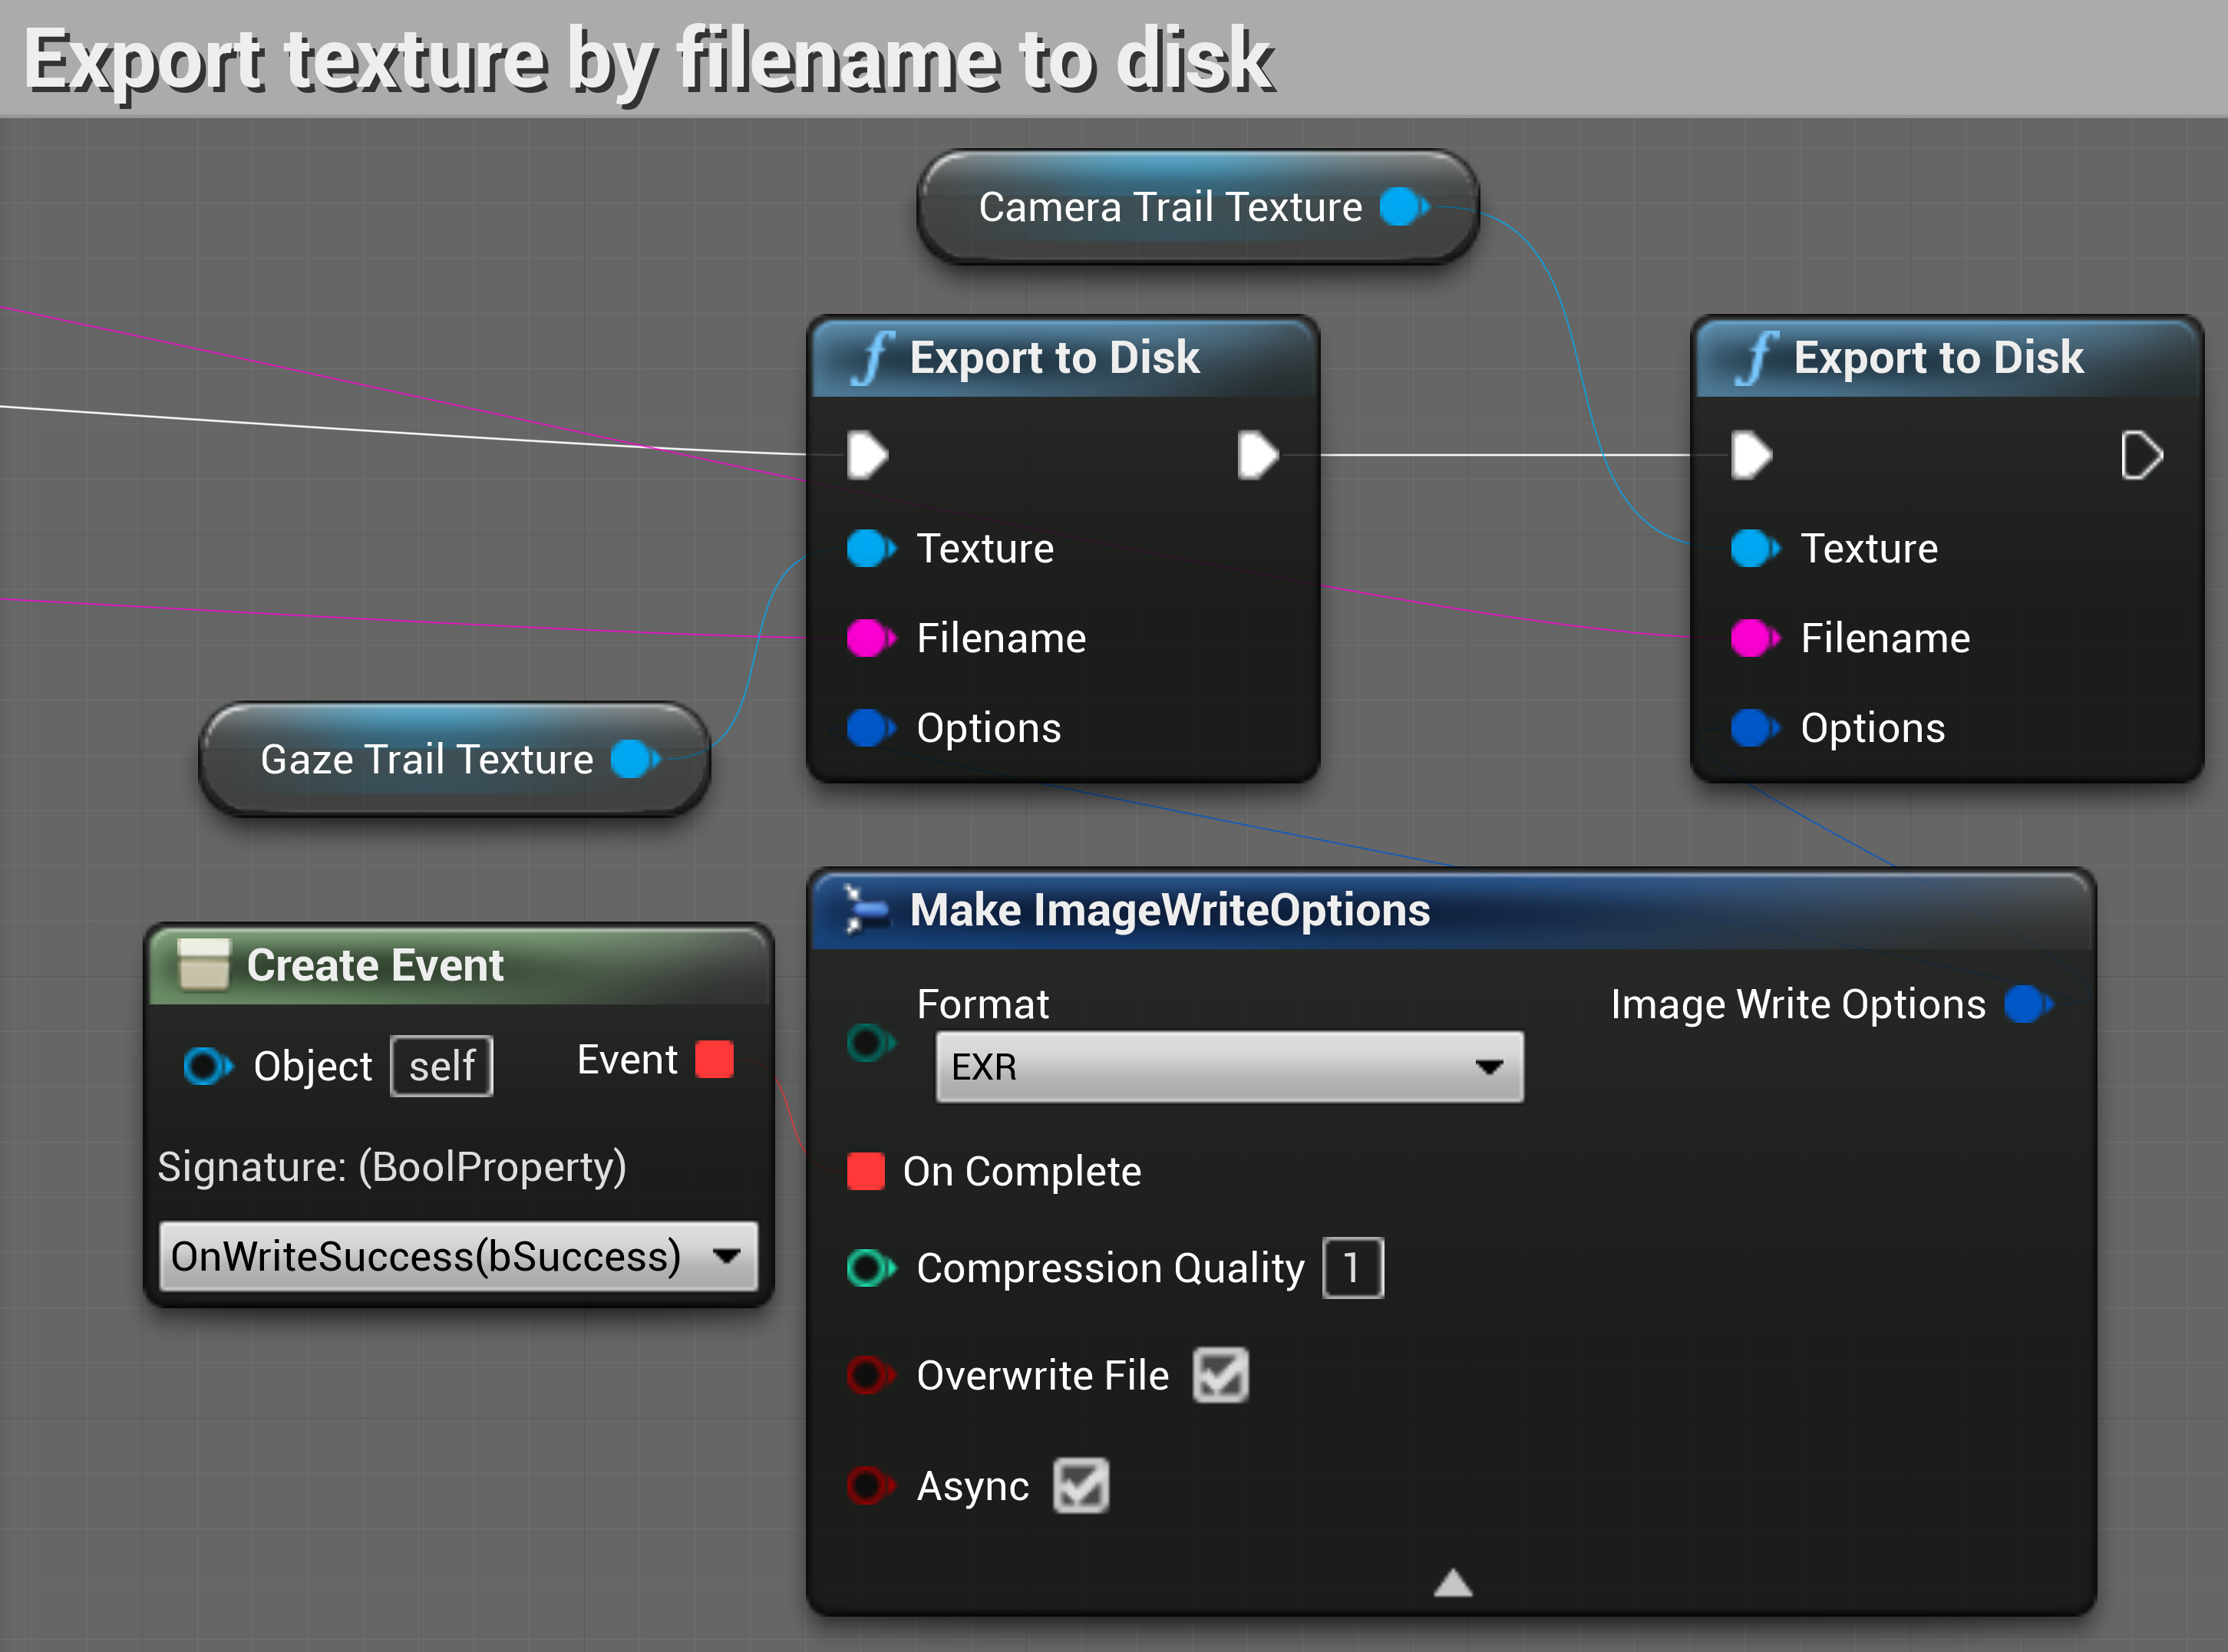
\includegraphics[width=\textwidth]{img/export-both-heatmap-textures.png}
    \caption{Export gaze and camera heatmap textures as EXR image format.}
    \label{fig:export-heatmaps-exr}
\end{figure}

\begin{figure}[!ht]
    \centering
    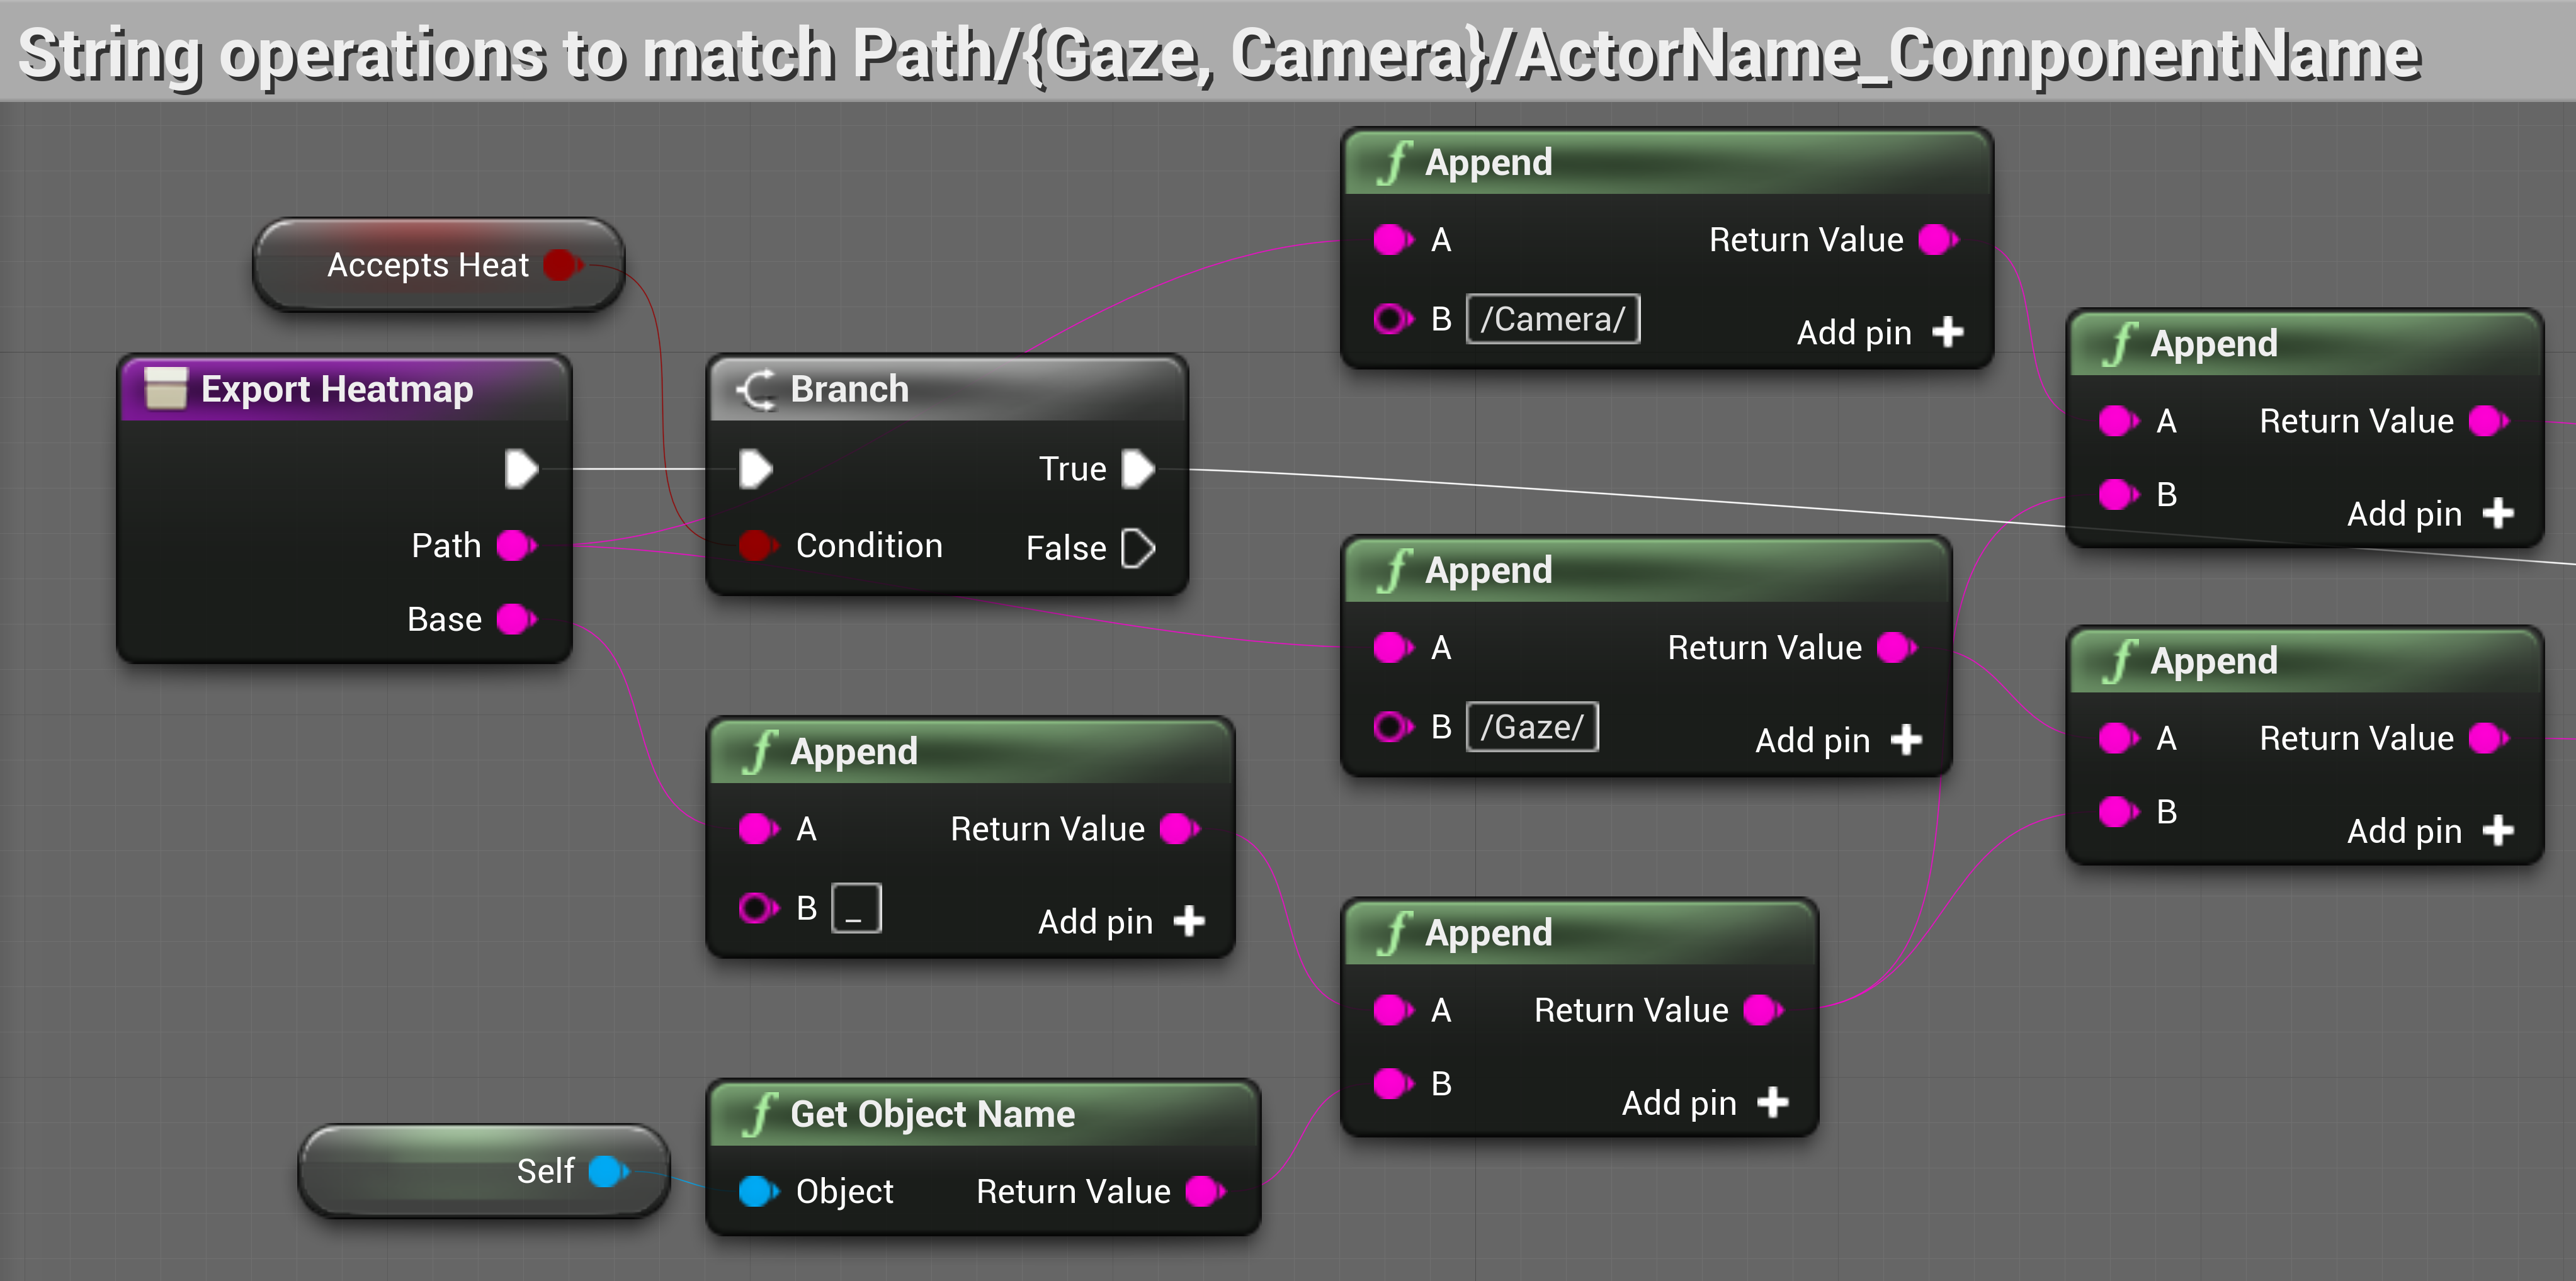
\includegraphics[width=\textwidth]{img/make-texture-filepath.png}
    \caption{Make filepath for the~exported gaze and camera heatmap textures.}
    \label{fig:make-filepath}
\end{figure}

\pagebreak{}

\subsection{HeatmapProducer}
\label{sec:uv-unwrap-implementation}
This class is used to produce heatmaps. Its design is based on the~analysis in Section~\ref{sec:uv-unwrap-method}. The~blueprint for recording unwrapped meshes is inspired by Tran's tutorial~\cite{tran2018wenderlich}. In order to function, it is absolutely necessary to insert this Actor into the~scene.

\begin{figure}[!ht]
    \centering
    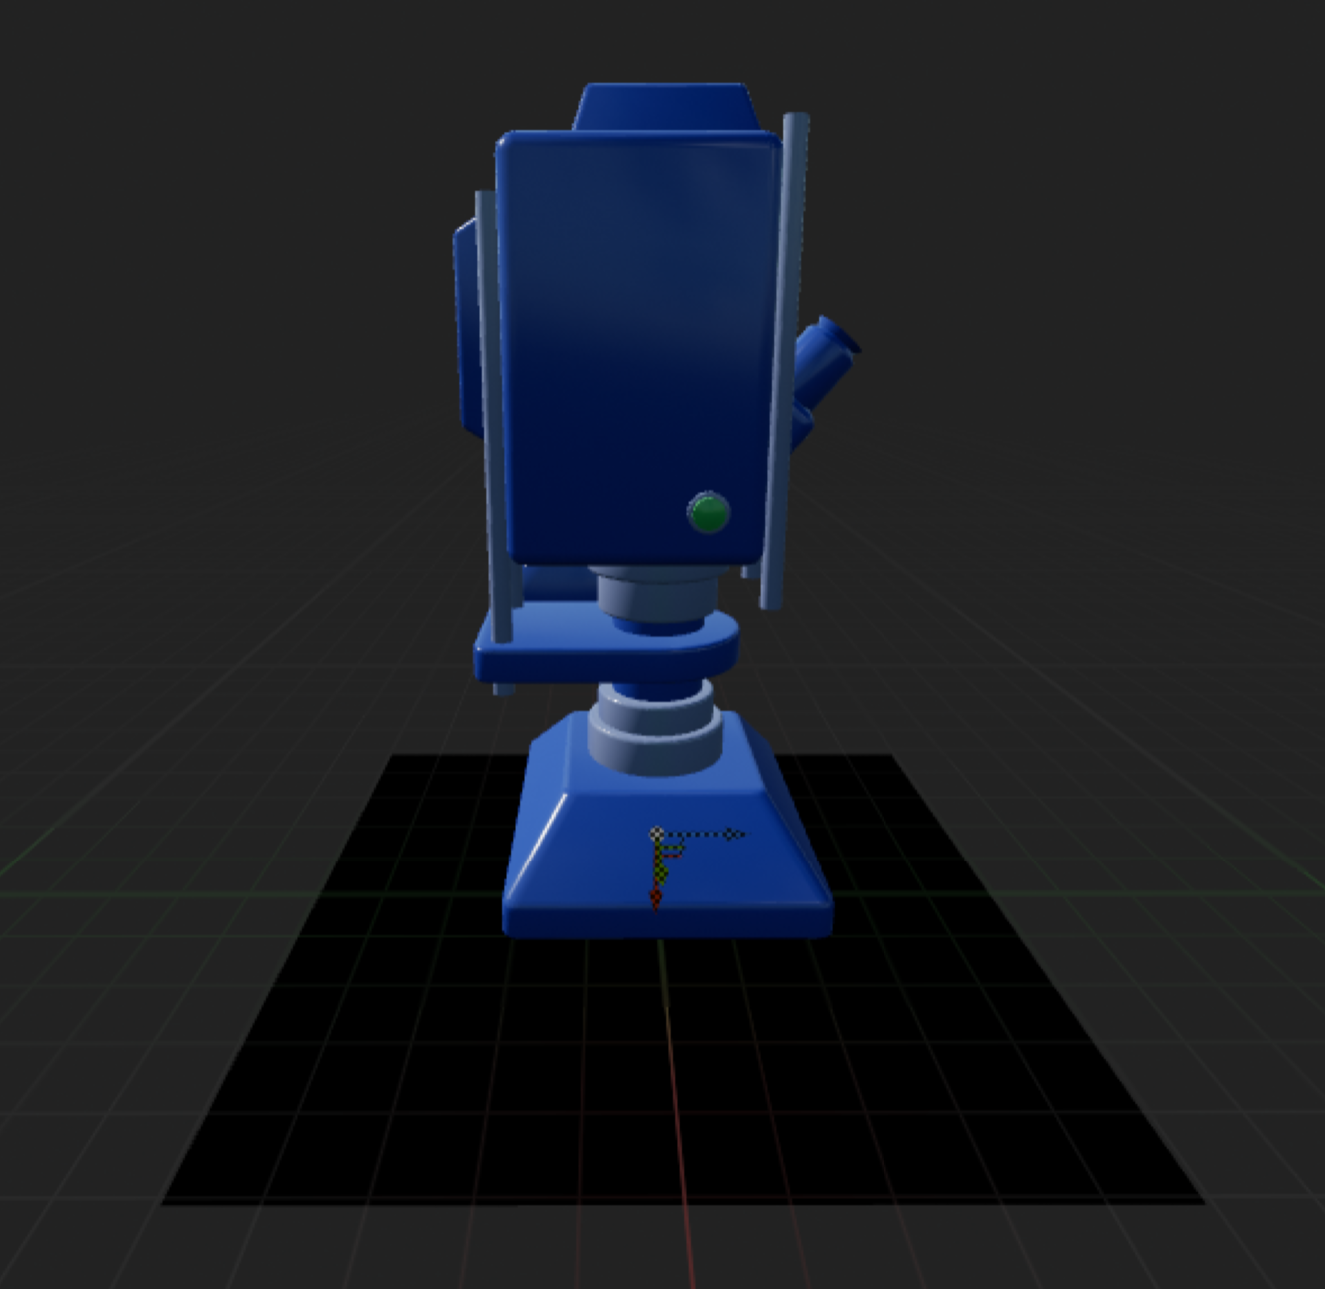
\includegraphics[width=0.4\textwidth]{img/heatmap-producer-viewport.png}
    \caption{HeatmapProducer capture component with background plane in viewport.}
    \label{fig:heatmap-producer-viewport}
\end{figure}

First, it is important to describe what the~Actor consists of. To record a~static mesh that unwraps itself into the~world according to its UV map, it is necessary to record the~state of this model with some kind of camera. This is what the~Scene Capture Component, with the~name of \emph{UnwrapUVCapture}, is for. To avoid recording unwanted effects from ambient lights and occlusion, the~camera is paired with a~simple plane to which a~UVRenderBackground material is added, which creates a~black background for the~mesh, as shown in Figure~\ref{fig:heatmap-producer-viewport}. The~camera is rotated $270{^\circ}$ on the~$z$ and $y$ axes to point directly at the~background. It is positioned higher than the~background, which is shifted to negative values of the~$z$-axis to avoid z-fighting with an~unwrapped mesh.  

The~capture component settings can be seen in Figure~\ref{fig:capture-component-settings}. The~camera must be of orthographic type and its width must correspond exactly to the~size of the~background plane. It is also critical to set the~Composite Mode to Additive, to ensure that capturing the~scene does not overwrite previous values but adds them to a~texture. The~background is a~square with a~100 cm long edge.

\begin{figure}[!ht]\centering
    \begin{subfigure}[b]{0.495\textwidth}
        \centering
        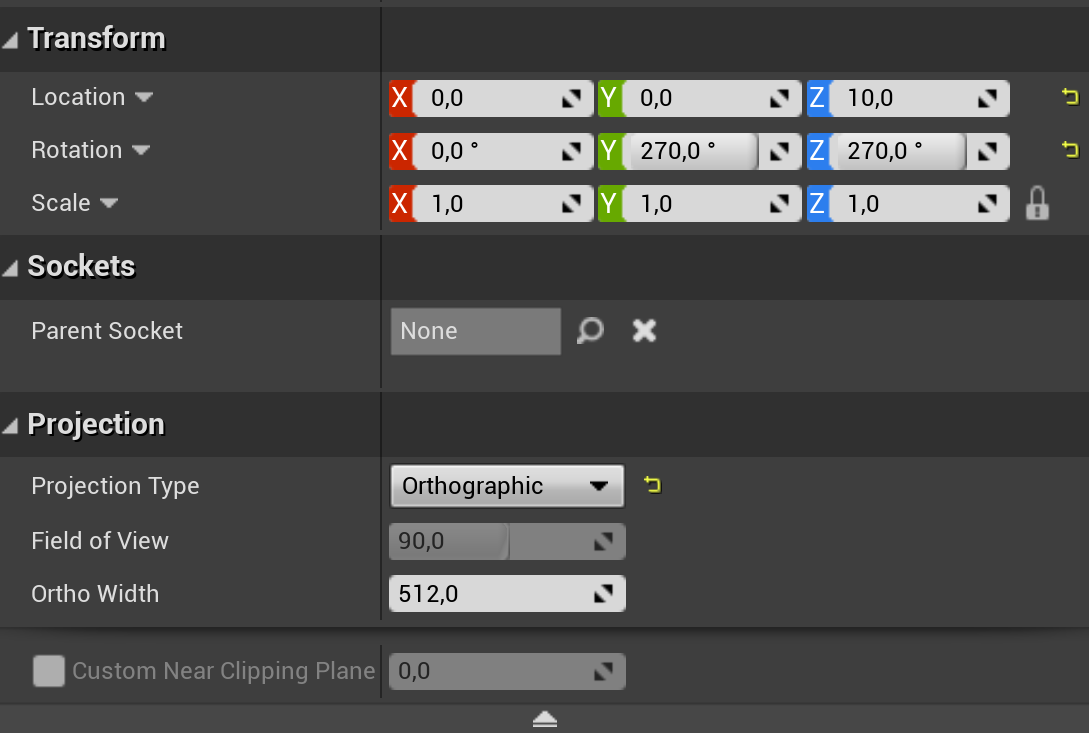
\includegraphics[width=\textwidth]{img/capture-component-settings.png}
    \end{subfigure}
    \hfill
    \begin{subfigure}[b]{0.495\textwidth}
        \centering
        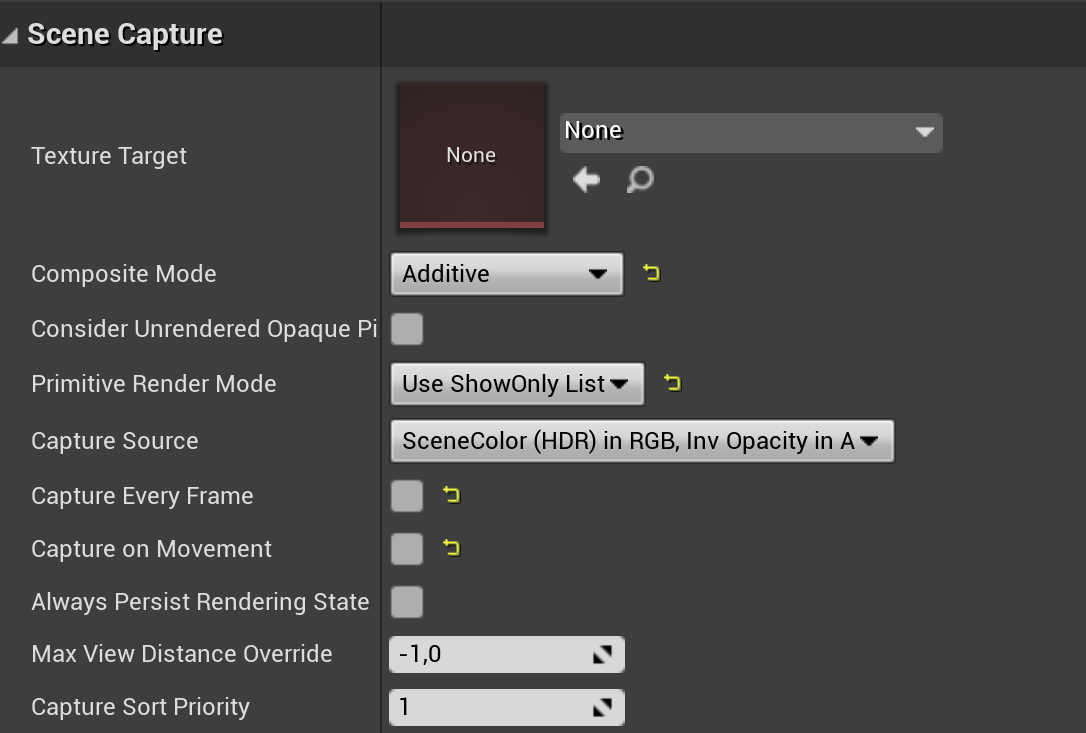
\includegraphics[width=\textwidth]{img/scene-capture-settings.png}
    \end{subfigure}
    \caption{UnwrapUVCapture Component settings.}
    \label{fig:capture-component-settings}
\end{figure}

\pagebreak{}

The~HeatProducer Actor contains a~private variable of the~dynamic material instance of UnwrapBrush material that is initialised in the~construction script of this Actor. Its parameters are described in Sections~\ref{sec:uv-unwrap-method} and \ref{sec:unwrap-brush-implementation}.

\subsubsection*{AlignRenderer function}

This function takes as input the~texture resolution and the~world position of an~unwrapped mesh. It is used to align the~two components of the~Actor and UnwrapBrush dynamic material instance parameters based on texture size and world position; that is, to avoid object culling, Section~\ref{sec:uv-unwrap-method}. To capture a~mesh into a~texture correctly, the~ortho width of the~capture component must first be set to the~exact resolution of the~texture. The~background must have its scale values on the~$x$ and $y$ axes adjusted to $t/100$, where $t$ is the~texture resolution in pixels, to be exactly the~same size as the~ortho width.

The~texture resolution is uploaded to the~dynamic material via the
\emph{CaptureSize} parameter and the~3D location of the~unwrapped object via the~\emph{UnwrapLocation} parameter.

\subsubsection*{PrepareScene}
The~PrepareScene function just takes an~EyeTrackedStaticMeshComponent and includes it along with the~black background in the~empty show-only list of the~capture component. 

\subsubsection*{ApplyHeatToComponent}

This function takes care of preparing the~HeatProducer Actor and the~component for rendering. As Figure~\ref{fig:apply-heat-function} shows, the~black background is first made visible, since it is normally not, then AlignRenderer is called according to the~resolution, the~PrepareScene function immediately after, and finally the~RenderSplatOntoComponent is called to render the~heatmap. It finishes by making the~background invisible again. 

\begin{figure}[!ht]
    \centering
    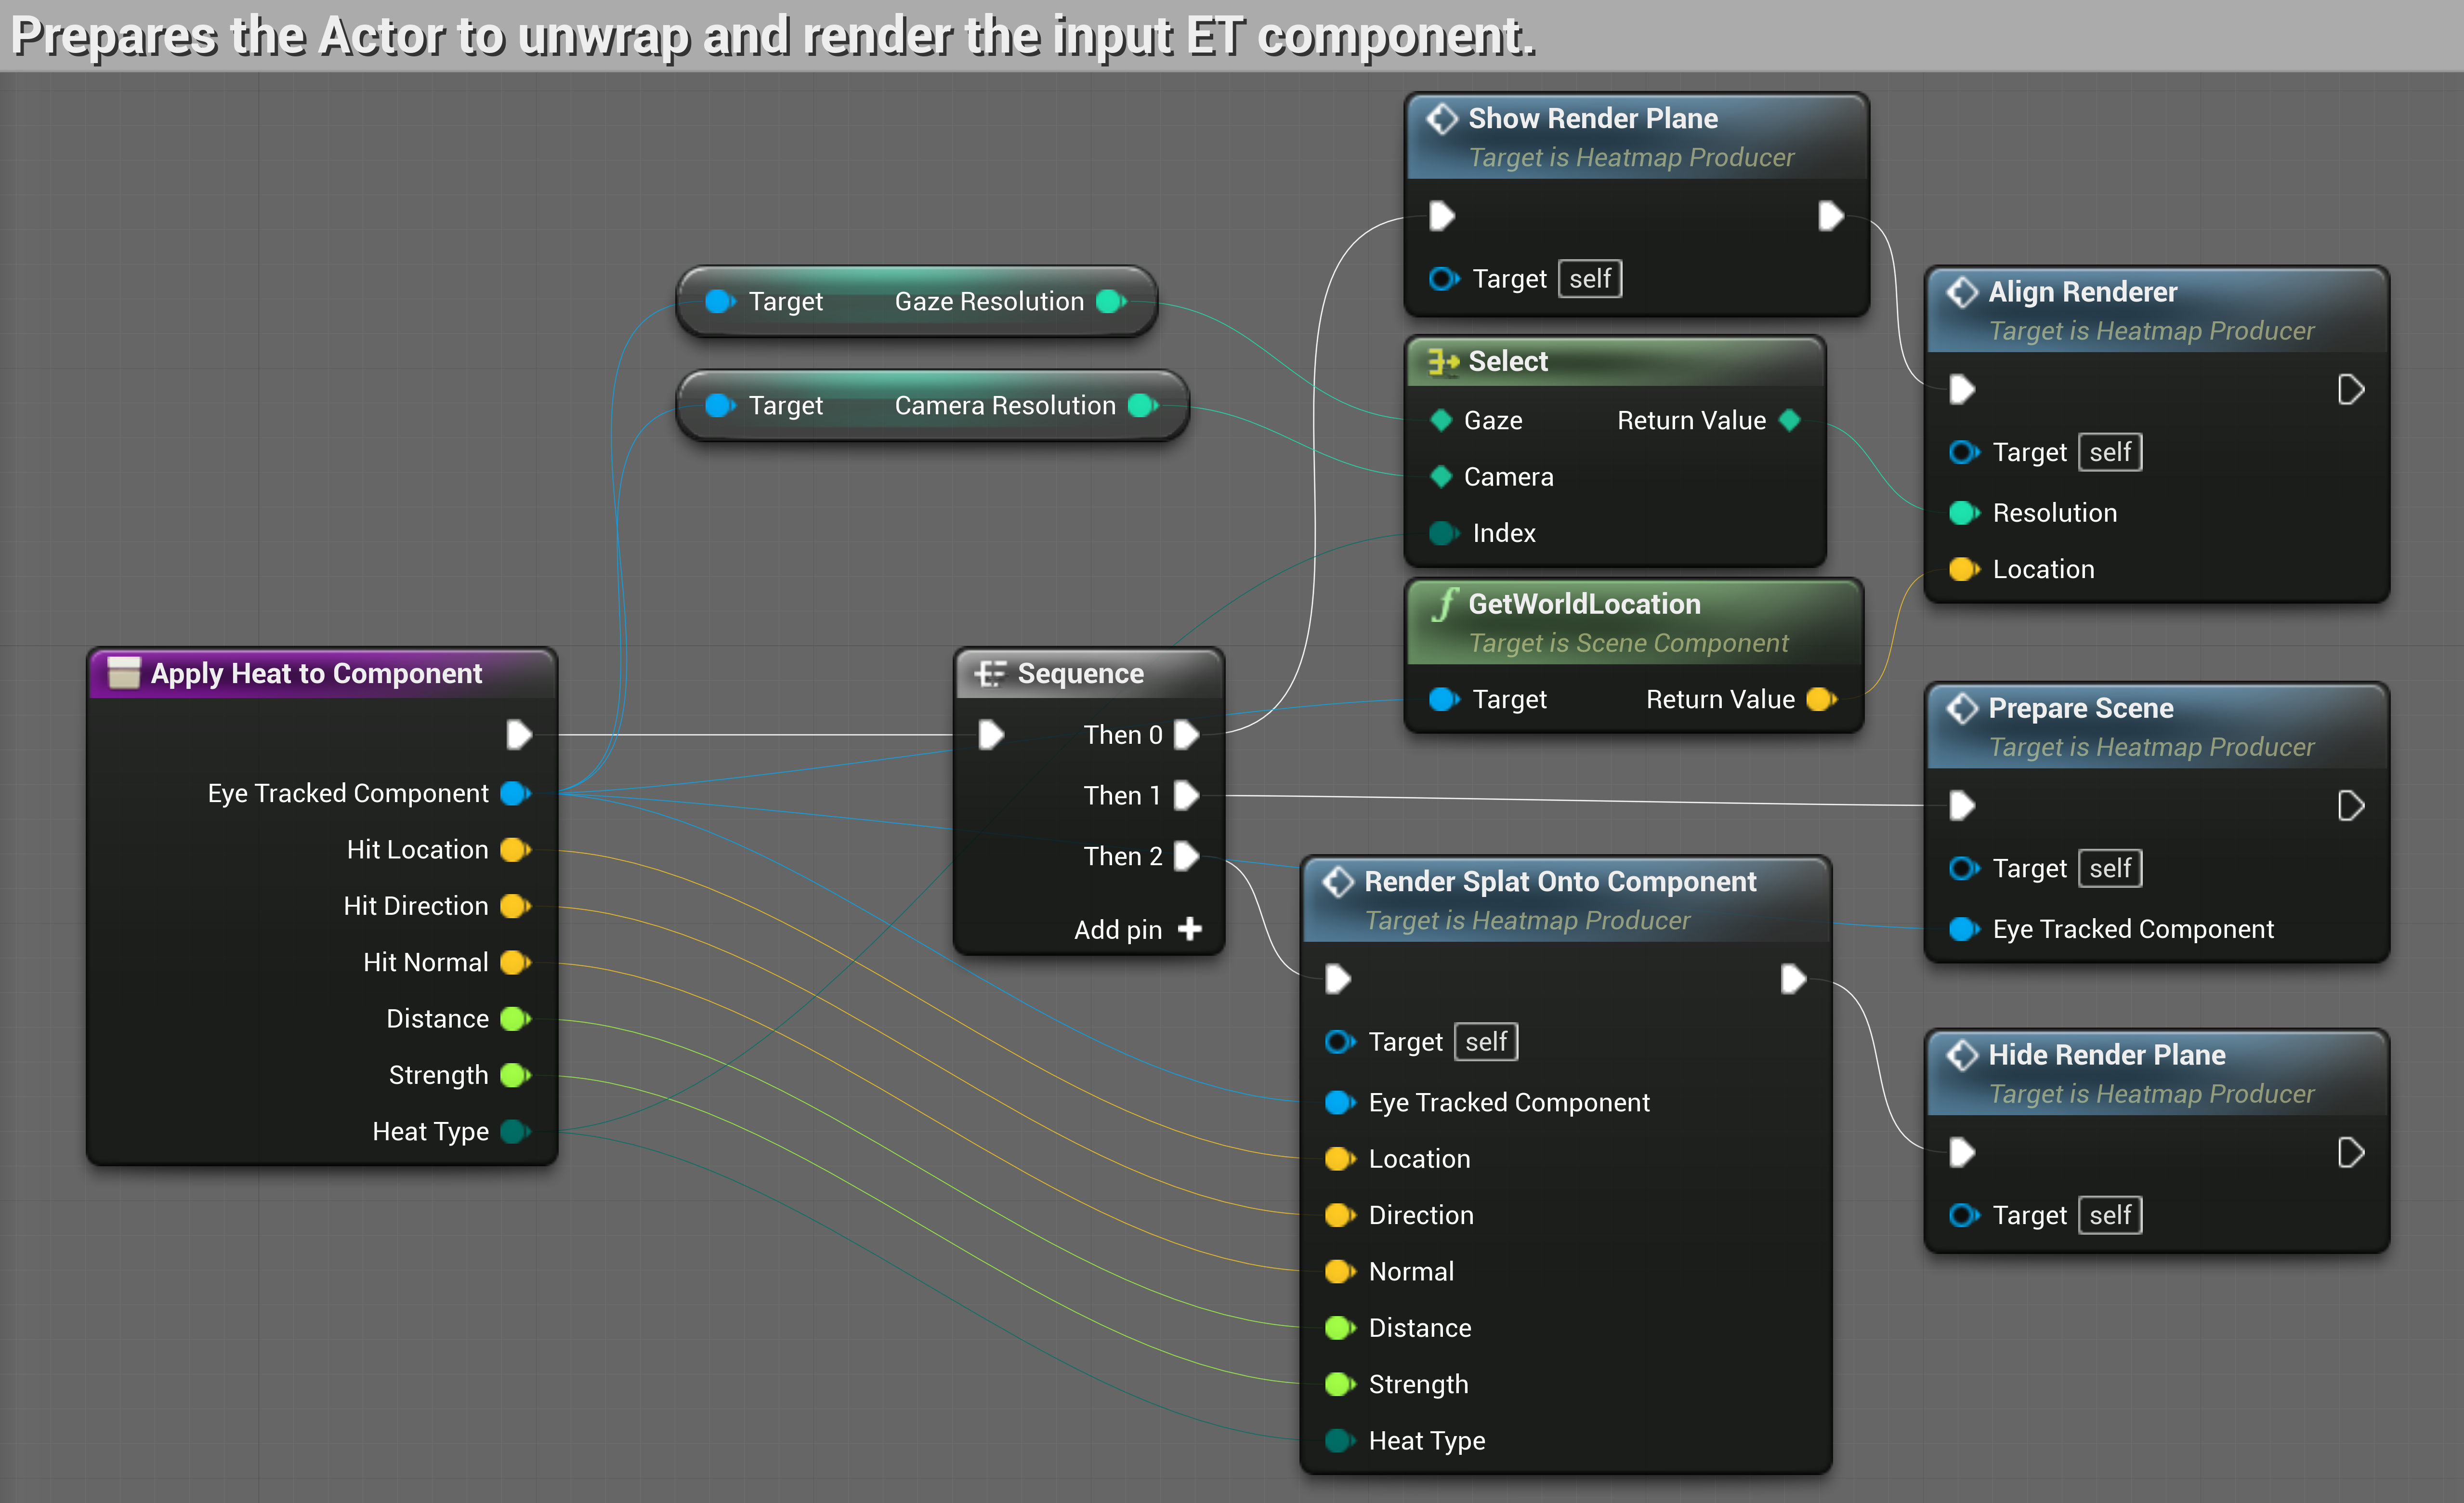
\includegraphics[width=\textwidth]{img/apply-heat-to-component.png}
    \caption{HeatmapProducer ApplyHeatToComponent function.}
    \label{fig:apply-heat-function}
\end{figure}

\subsubsection*{RenderSplatOntoComponent}

This is a~function of many inputs. Namely, Location, Direction (from camera), Normal, Distance, and Strength. All of them correspond to all the~remaining parameters of the~UnwrapBrush material, which are set exactly as the~previous cases of dynamic material parameters, for example, Figure~\ref{fig:load-heatmap-textures}. These are HitLocation, DirectionToCamera, HitNormal, BrushRadius, and Strength.

Next, the~original material of the~component is stored in a~local variable, because its material is immediately replaced by the~UnwrapBrush instance. This can be seen in Figure~\ref{fig:render-splat-function}. Thus, it is immediately rendered, after a~render target has been assigned to it, using the~Capture Scene function. At this point, a~new value is added to the~render target according to UnwrapBrush. The~function ends by returning the~component its original material. 

\begin{figure}[!ht]\centering
    \begin{subfigure}[b]{\textwidth}
        \centering
        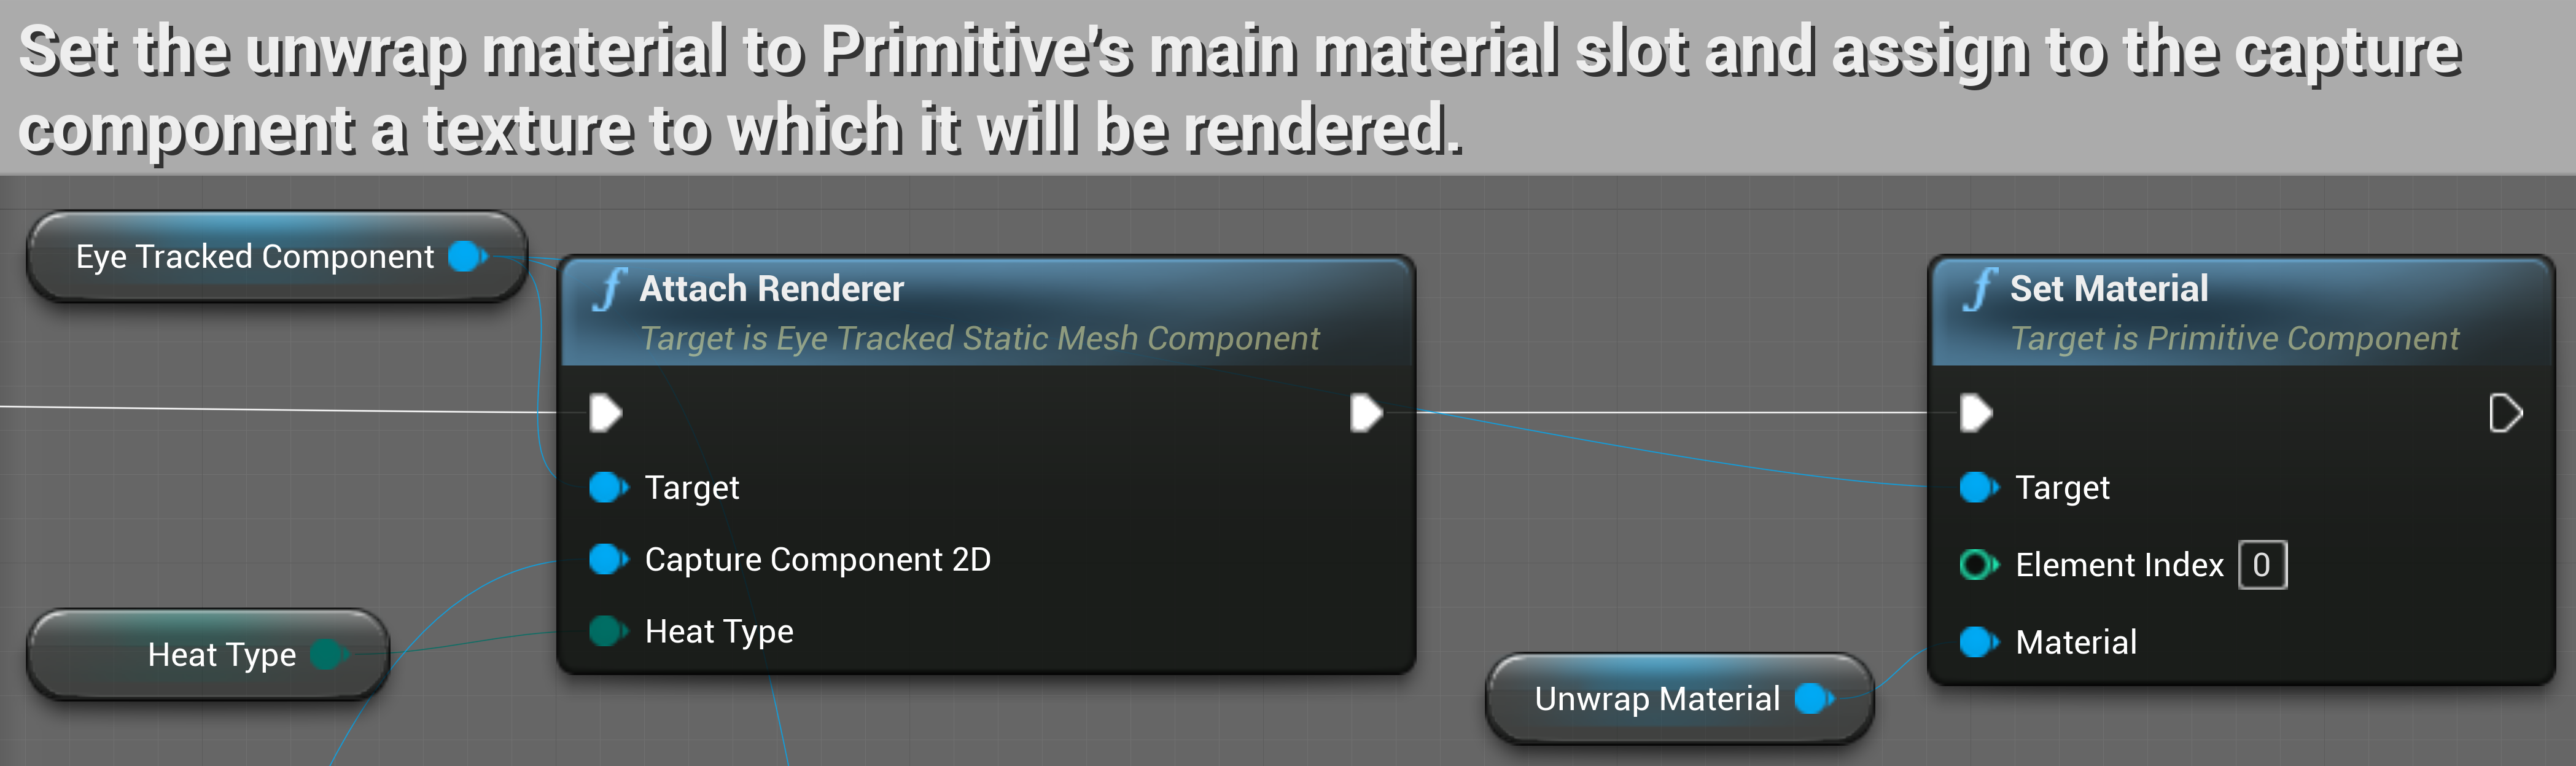
\includegraphics[width=\textwidth]{img/render-splat-1.png}
    \end{subfigure}
    \hfill
    \begin{subfigure}[b]{\textwidth}
        \centering
        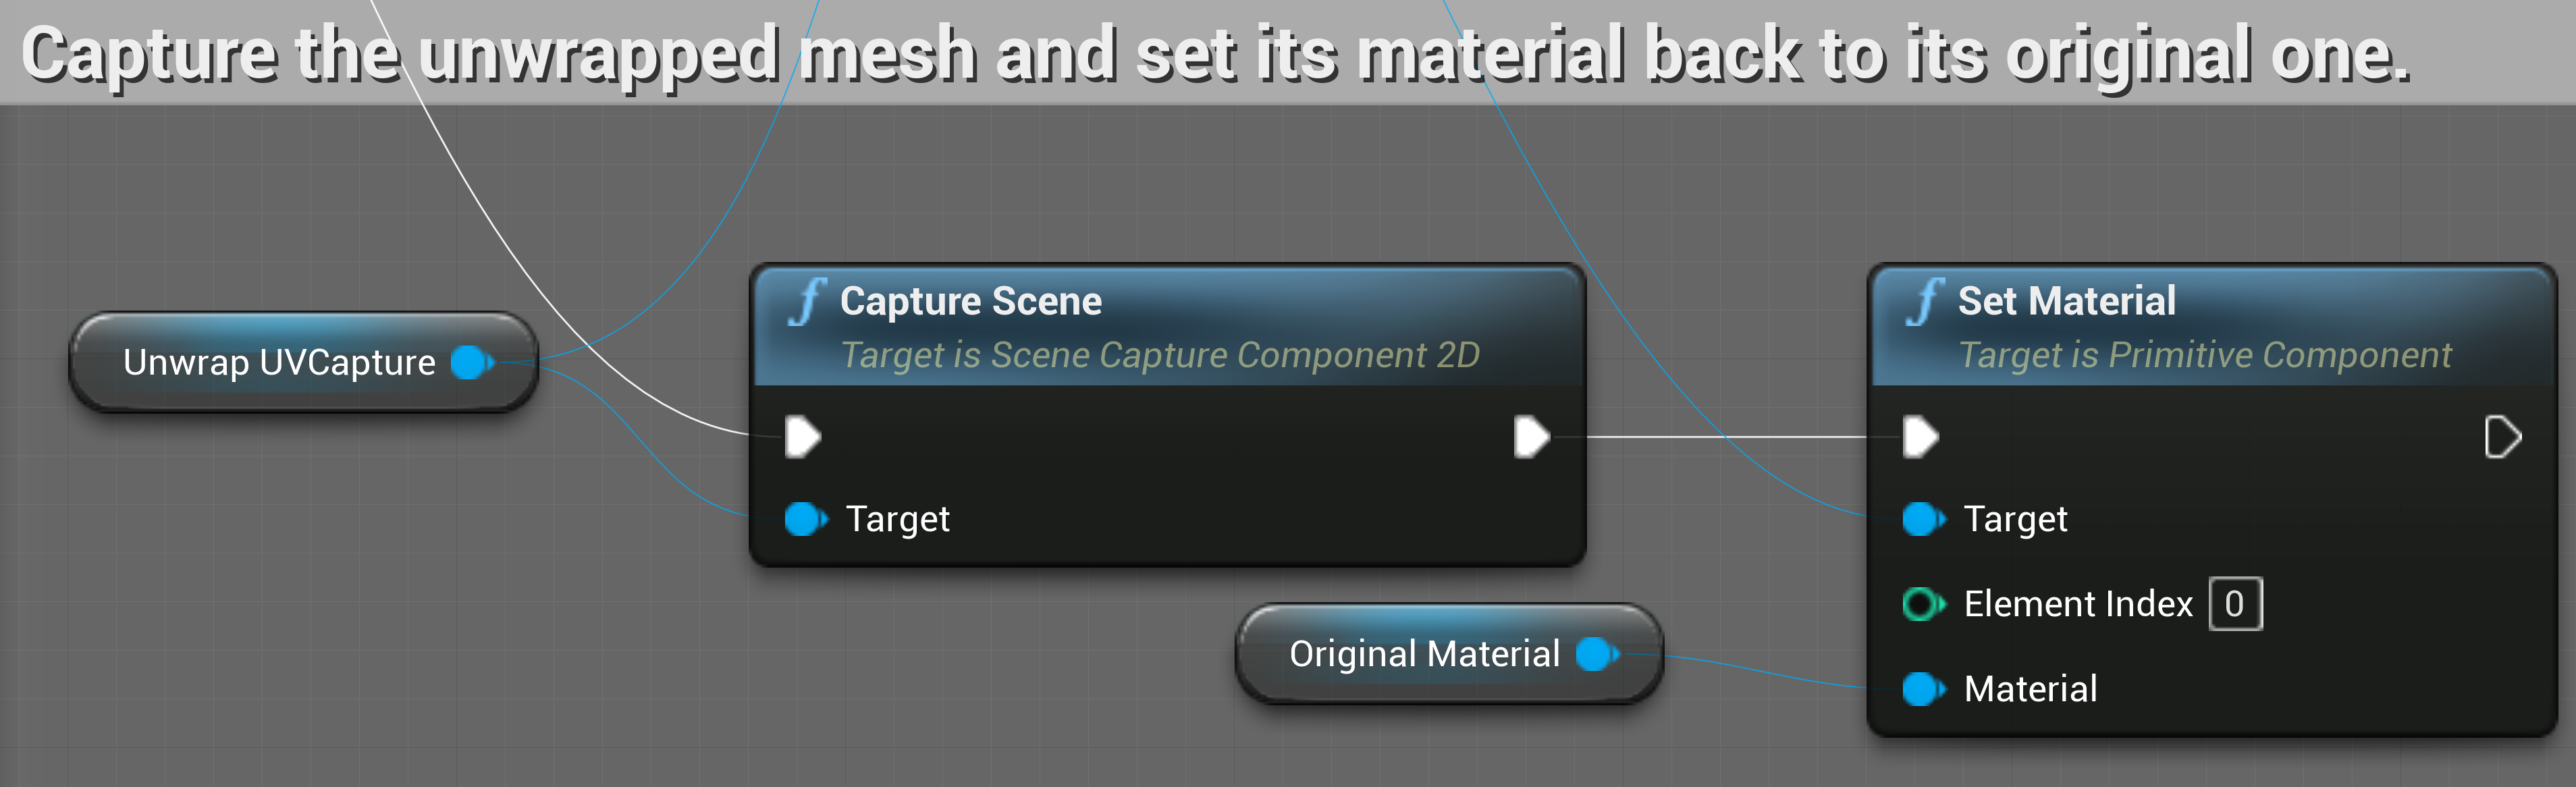
\includegraphics[width=\textwidth]{img/render-splat-2.png}
    \end{subfigure}
    \caption{HeatProducer RenderSplatOntoComponent function.}
    \label{fig:render-splat-function}
\end{figure}

\subsection{GazeEmitter}
\label{sec:gaze-emitter}

It is a~child of the~SceneComponent class and is crucial for the~whole plug-in functionality. It is intended to be added to some user-defined Pawn. After that, the~user can define what they want to use as input to this plug-in. If they wanted to track a~character moving around the~floor of the~scene, all they would need to supply GazeEmitter with is the~position of the~character and a~directional vector to the~ground. This would cause heatmaps to be created on the~floor object, which would be defined as an~EyeTrackedStaticMeshComponent.

At the~beginning of the~game, the~component is constructed and in its \emph{BeginPlay} event, it contains the~spawn node of the~HeatmapProdurer Actor and its assignment to a~private variable, as can be seen in Figure~\ref{fig:emitter-begin}.

\pagebreak{}

\begin{figure}[!ht]
    \centering
    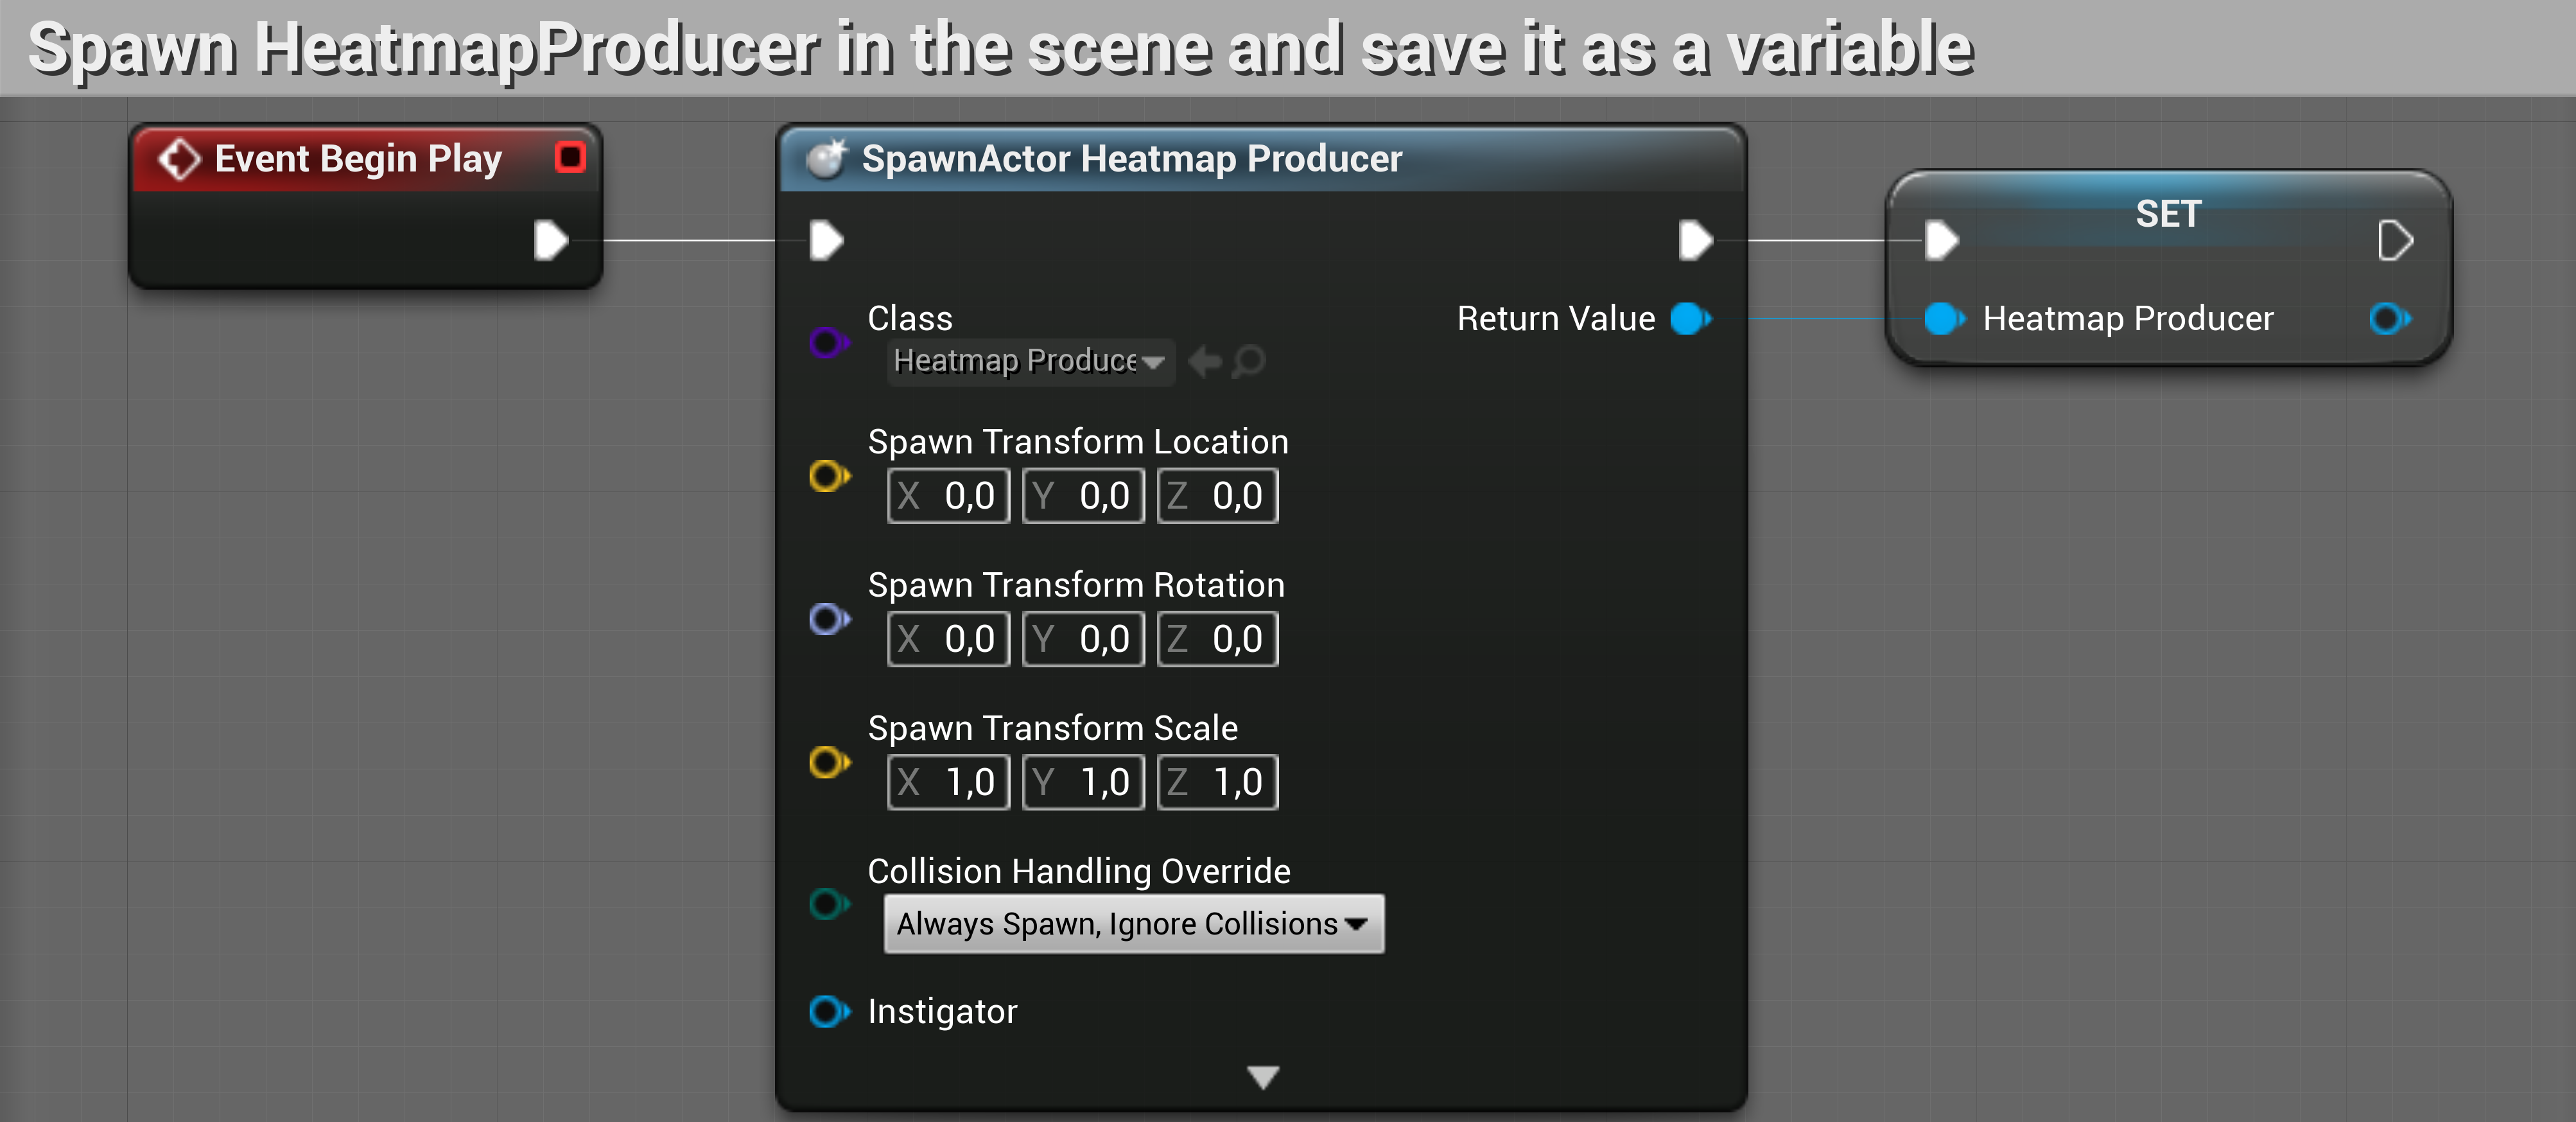
\includegraphics[width=\textwidth]{img/gaze-emitter-begin-play.png}
    \caption{GazeEmitter Event BeginPlay.}
    \label{fig:emitter-begin}
\end{figure}

The~whole functionality consists only of calling \emph{LineTraceForObjects}, which passes the~start and end of a~trace ray that detects a~collision on some object in the~scene. This is done using the~\emph{GetWorldHitFrom} function in Figure~\ref{fig:emitter-world-hit}. If it hits something, it first determines if it is an~EyeTrackedStaticMeshComponent; if so, the~trace was successful.

This first trace was only performed as part of a~simple collision to first know which component is being hit. It cannot be guaranteed that the~simple collision volume will be detailed enough to represent the~entire mesh. If heatmaps were drawn only under these circumstances, it might happen that heat would not be applied to some parts of several objects. Illustrated in the~video with the~path \path{video/03-simple-collision-only.mp4}.

There is a~function in Unreal called \emph{LineTraceComponent} that takes a~component and the~start and end of a~trace ray as input. Its advantage is that it only performs the~tracing on that particular component. Tracing can be set to complex, which will traverse all triangles of a~given mesh to find a~collision. For meshes with a~very high triangle count, this can be a~time consuming operation. 

This is handled by GazeEmitter's \emph{GetComplexFromSimpleHit} function also in Figure~\ref{fig:emitter-world-hit}, which takes a~hit as input, extracts the~trace ray, and sends it again. The~general functionality of creating heatmaps using these functions can be seen in the~\path{video/04-creating-heatmaps.mp4} using a~forward vector of a~virtual camera.

\begin{figure}[!ht]
    \centering
    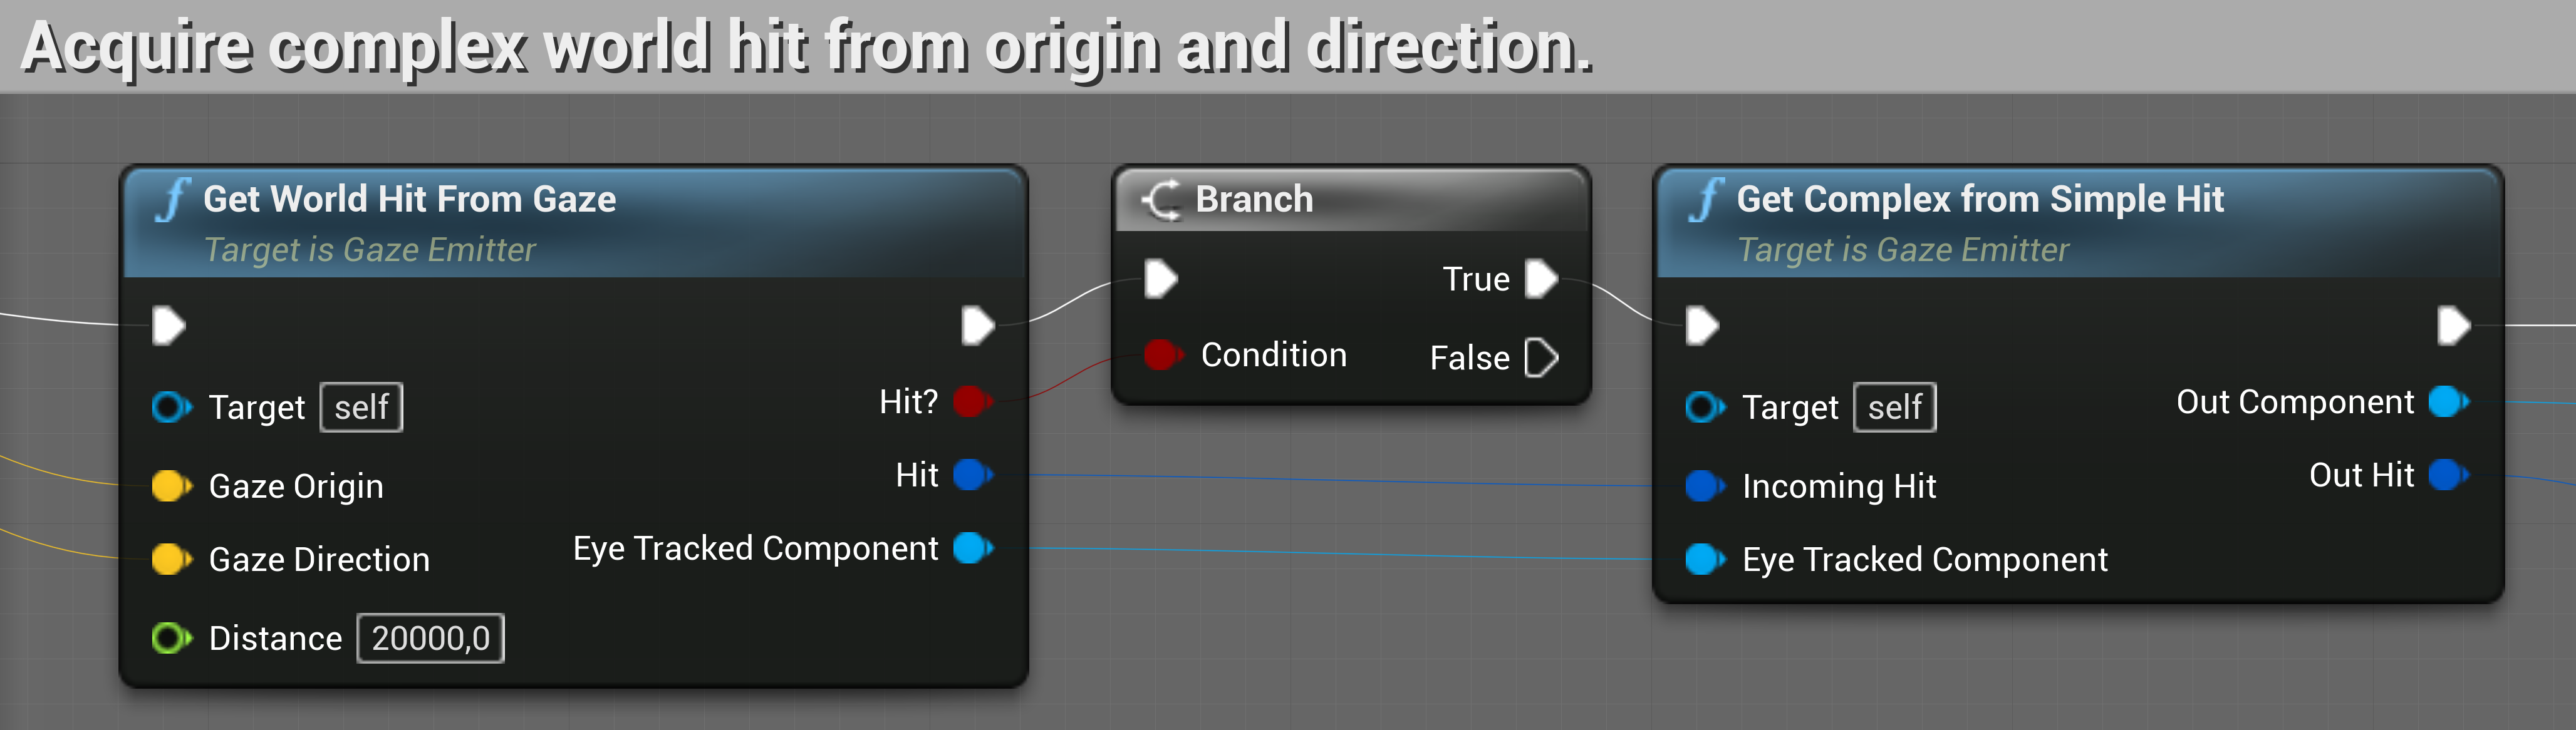
\includegraphics[width=\textwidth]{img/ray-world-hit.png}
    \caption{GazeEmitter get a~complex world hit on a~single component.}
    \label{fig:emitter-world-hit}
\end{figure}

\pagebreak{}

\section{Python}
\label{sec:python}
The~Python section will describe the~script for producing the~resultant data from the~collected EXR textures from different users.

\subsection{EXR image merger script}

This script is used to edit EXR files by iterating through all possible textures of one measurement and one type. This gives a~unique texture for all objects that were part of the~Unreal scene.

\medskip{}
However, these textures exist in multiple variations, depending on how many measurements were made. As a~merging script, it ensures that all these textures are merged into one. This is done simply by dividing all texture values by the~number of variants. These weighted textures are then merged by a~simple add operation.

\medskip{}
For this, the~OpenEXR library~\cite{openexr} is used to perform read and write operations on EXR files, and NumPy~\cite{numpy-doc} to perform these image operations.

\medskip{}
The~OpenXR library always reads the~image channels as strings. Now, it depends on how the~textures are defined. They can be of 32 and 16 bit floats. In the~case of exported textures, they are 16-bit EXR images. Using NumPy, this string is converted just according to \path{numpy.float16}.

\bigskip{}
The~script gets the~paths to all texture files of a~single scene object. Individually reads their red channel as a~string, which is converted to a~numpy array. Creates an~empty 1D 16-bit float buffer of the~size of the~texture's pixel count. Then, it successively loads each red channel of all the~textures into this buffer, multiplied by a~weight constant. The~resultant numpy array is converted back to a~string and exported by the~OpenEXR function, where the~red channel is assigned for both the~green and blue channels. This can be done because the~heatmap trail is a~white image. The~commented source code can be found in the~enclosed media in \path{src/python/merger.py}. 




% \definecolor{codegreen}{rgb}{0,0.6,0}
% \definecolor{codegray}{rgb}{0.5,0.5,0.5}
% \definecolor{codepurple}{rgb}{0.58,0,0.82}
% \definecolor{backcolour}{rgb}{0.95,0.95,0.92}

% \lstdefinestyle{mystyle}{
%     backgroundcolor=\color{backcolour},   
%     commentstyle=\color{codegreen},
%     keywordstyle=\color{magenta},
%     numberstyle=\tiny\color{codegray},
%     stringstyle=\color{codepurple},
%     basicstyle=\ttfamily\footnotesize,
%     breakatwhitespace=false,         
%     breaklines=true,                 
%     captionpos=b,                    
%     keepspaces=true,                 
%     numbers=left,                    
%     numbersep=5pt,                  
%     showspaces=false,                
%     showstringspaces=false,
%     showtabs=false,                  
%     tabsize=2
% }

% \lstset{style=mystyle}

% \lstinputlisting[caption={EXR Heatmap Texture merger script~}, captionpos=b, language=Python]{code/merger.py}

\chapter{Experiment}
\begin{chapterabstract}
This chapter will describe the~production of the~experiment scene. It deals with the~transfer of the~original model to the~Unreal Engine project and finally with the~deployment of the~plug-in produced in Chapter~\ref{chap:implementation}.
\end{chapterabstract}

\section{Scene}
The~scene was made in Blender~\cite{blender} and transferred to an~Unreal project, which can be found in the~enclosed media in the~\path{experiment/project/CNB_NC_ET.zip} file. Opening this unreal project may require compilation. All later introduced Blueprints are found in this project. The~entire level in the~Unreal project can be seen in Figure~\ref{fig:unreal-cnb-level}.

\begin{figure}[!ht]\centering
    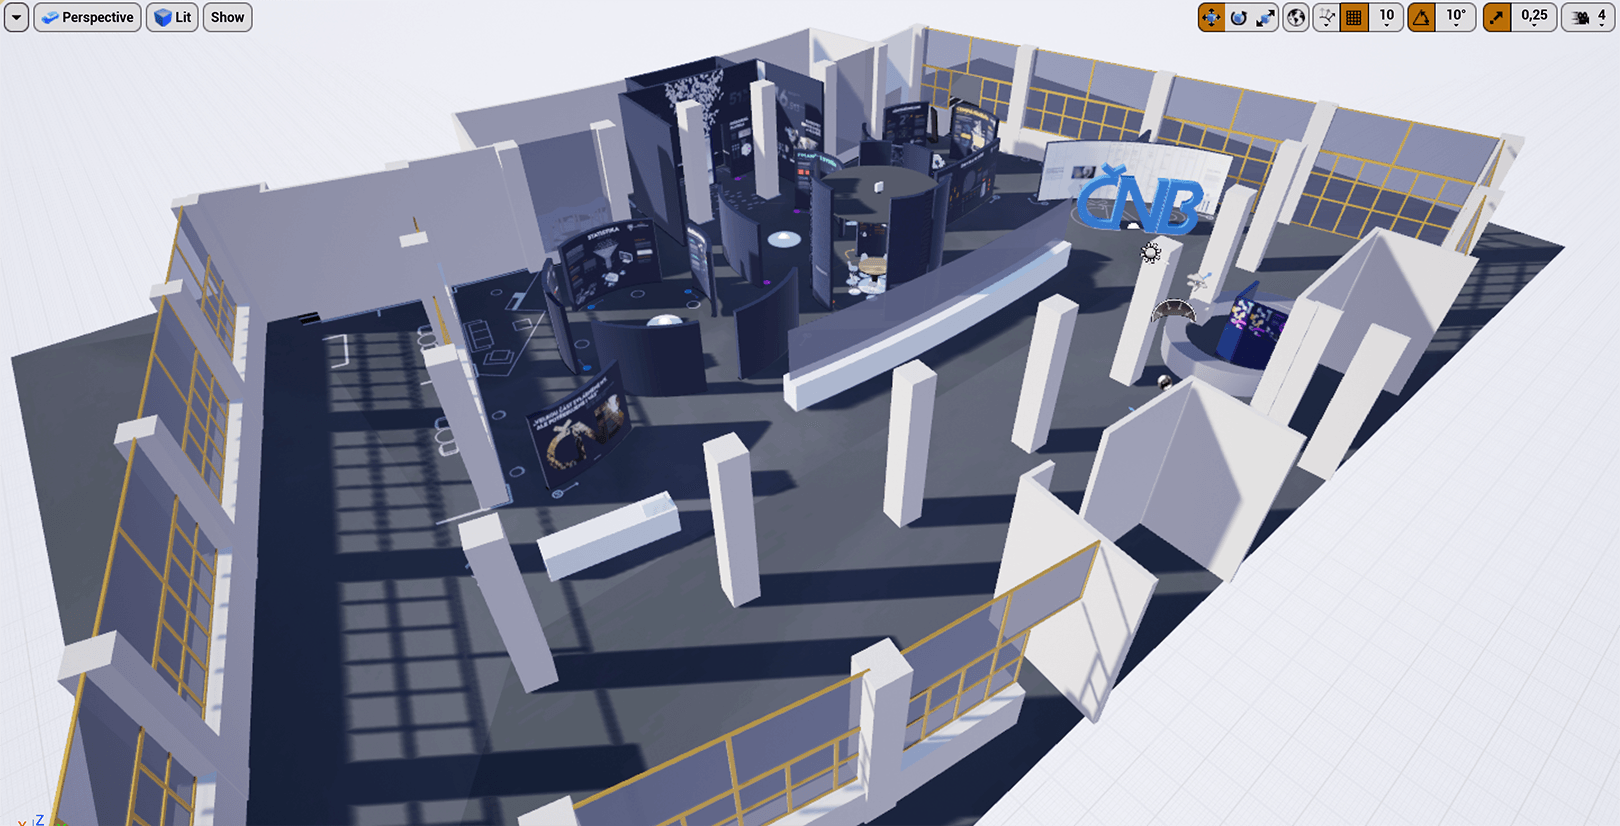
\includegraphics[width=\textwidth]{img/unreal-cnb-scene.png}
    \caption{NC\_ET Level of CNB\_NC\_ET Unreal project.}
    \label{fig:unreal-cnb-level}
\end{figure}

\pagebreak{}
\subsection{Czech National Bank Visitor Centre}
The~scene produced for the~ET experiment is a~Visitor Centre exhibition at the~Czech National Bank~\cite{cnb-nc}. AV MEDIA SYSTEMS, a.s., which was part of this project, internally created a~model of this exhibition in Blender for prototyping purposes~\cite{cnb3dmodel}, the~model can be seen in Figure~\ref{fig:blender-cnb-level}. This prototype was not involved as part of the~construction process. See Figure~\ref{fig:real-cnb-level} where the~exhibition can be seen in a~construction process. Ahrend,~a.s. was responsible for the~realisation of this exhibition in cooperation with AV MEDIA SYSTEMS,~a.s..

\begin{figure}[!ht]\centering
    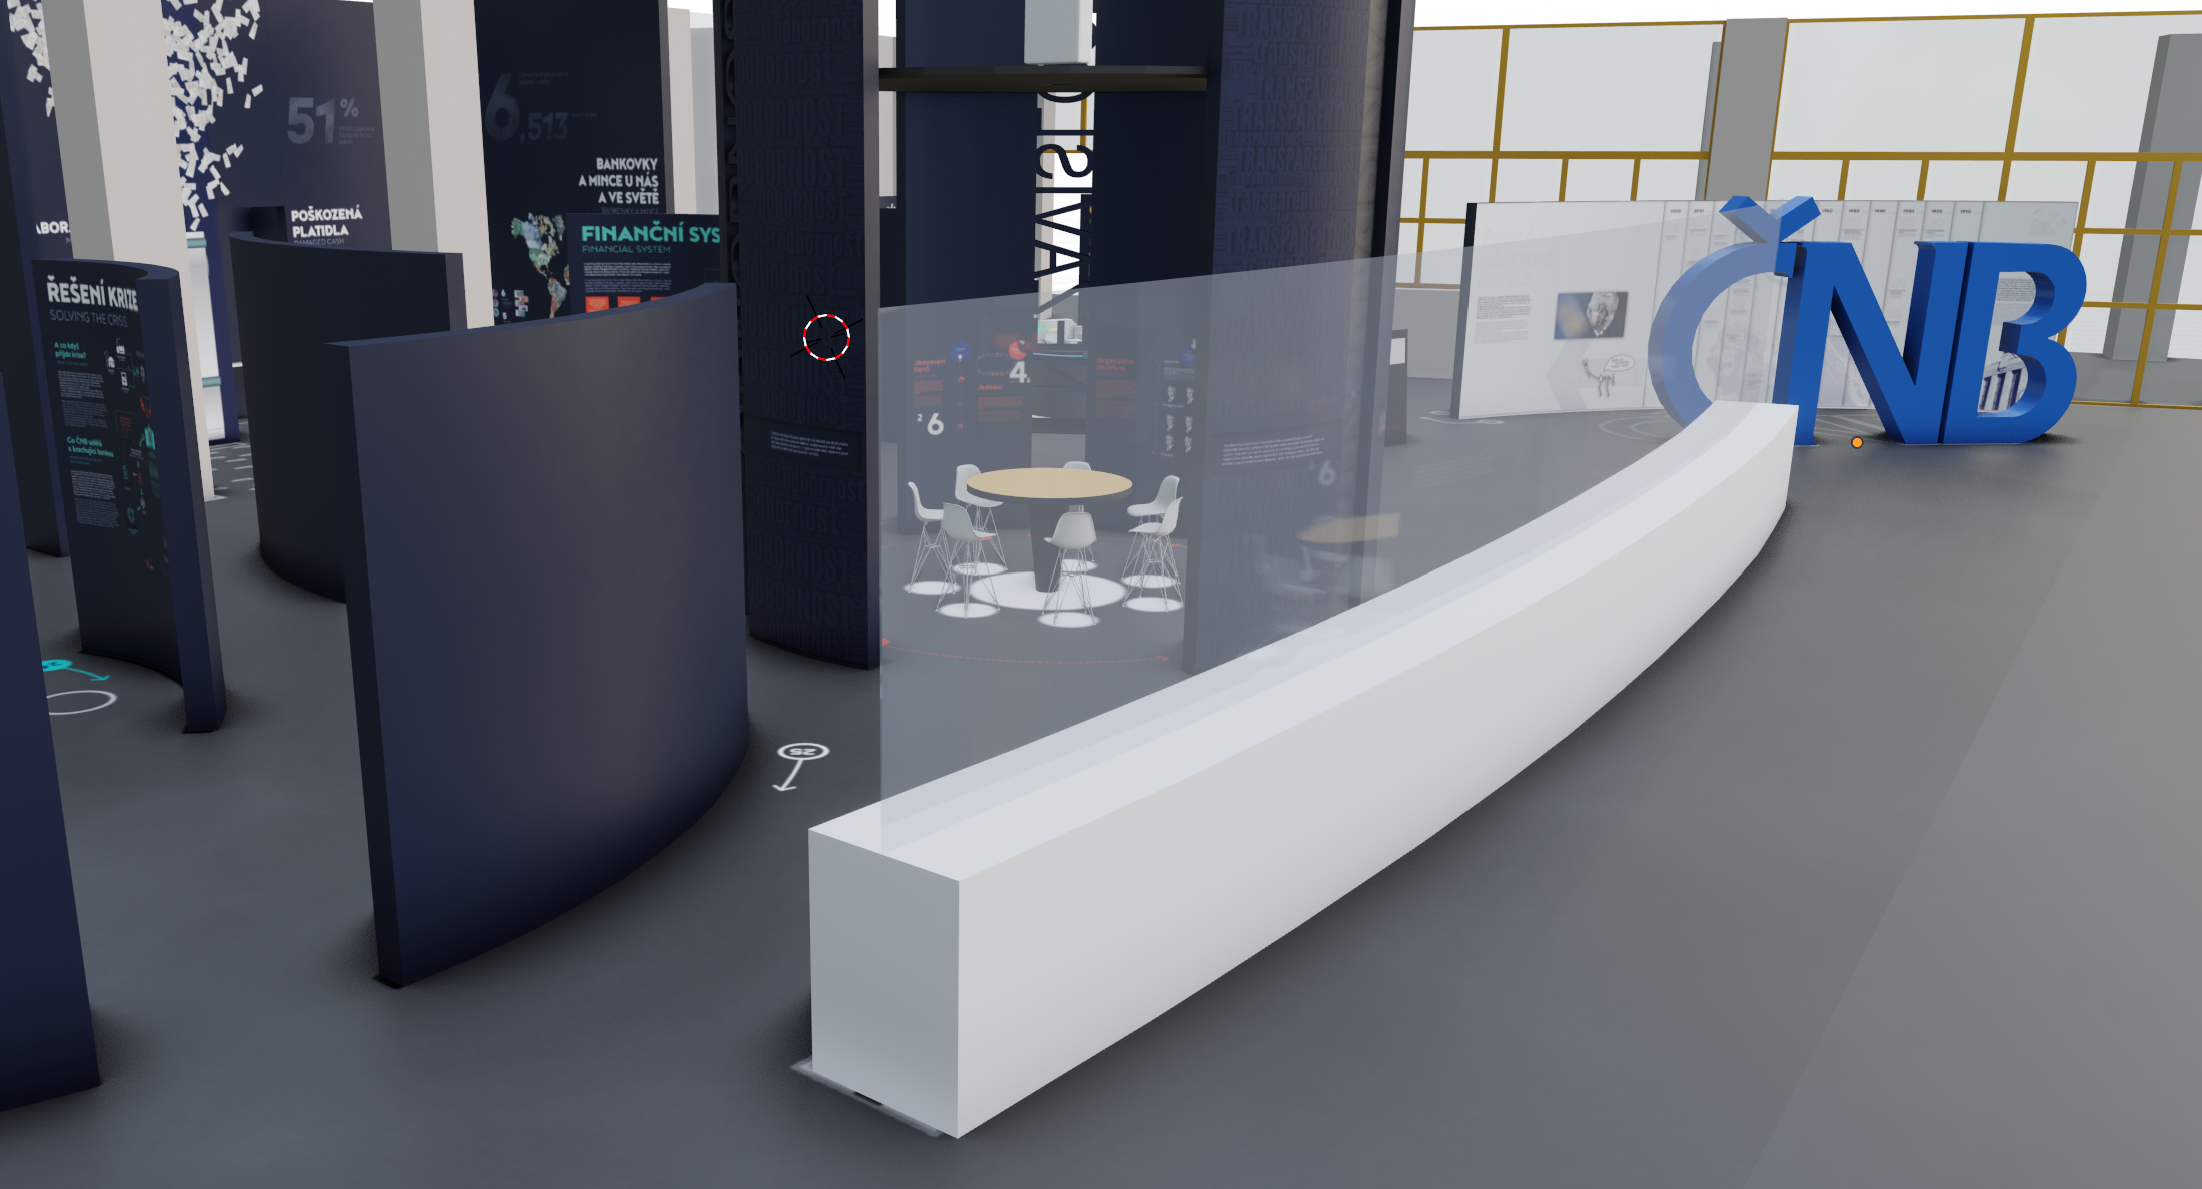
\includegraphics[width=\textwidth]{img/blender-cnb-scene.png}
    \caption[AV MEDIA SYSTEMS, a.s. internal prototype Blender model of CNB Visitor Centre.]{AV MEDIA SYSTEMS, a.s. internal prototype Blender model of CNB Visitor Centre.~\cite{cnb3dmodel}}
    \label{fig:blender-cnb-level}
\end{figure}

\begin{figure}[!ht]\centering
    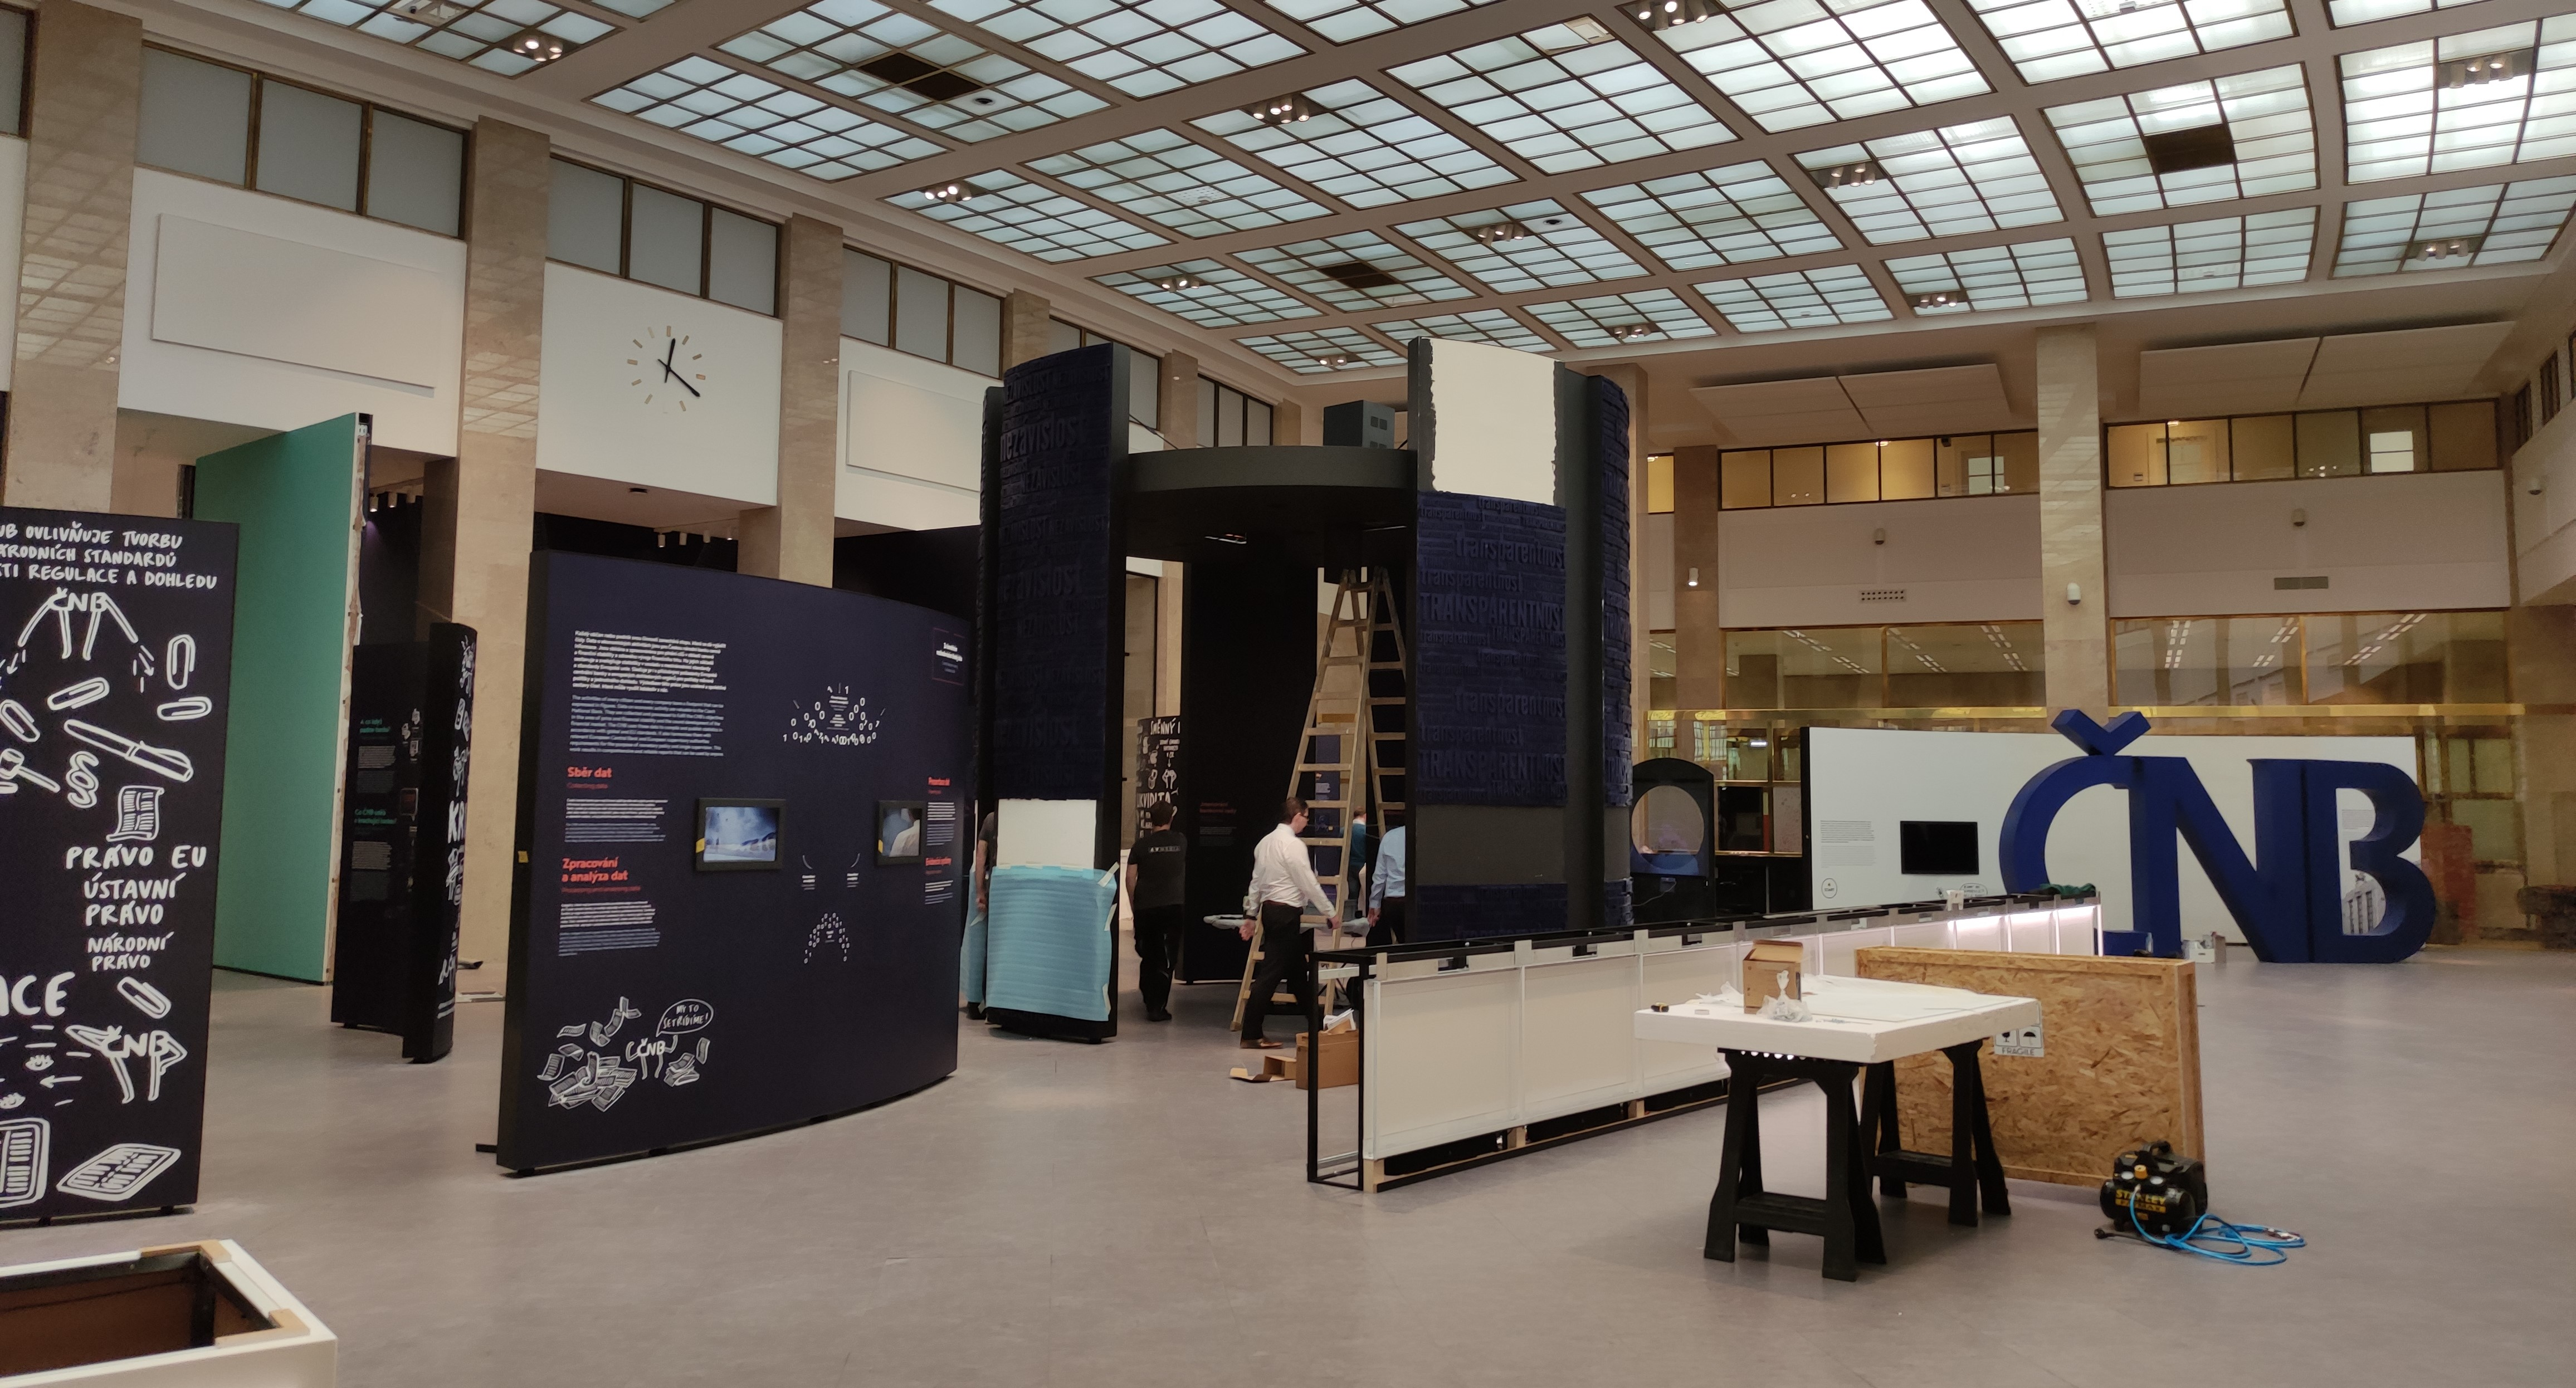
\includegraphics[width=\textwidth]{img/real-cnb-scene.jpg}
    \caption{Visitor Centre of Czech National Bank during construction.}
    \label{fig:real-cnb-level}
\end{figure}

\section{Scene modification}
The~way the~Unreal Engine requires the~definition of objects in levels along with the~definition of the~functionality of the~created plug-in, it would be impractical to convert this model to the~Unreal scene in its original state. This section defines issues with the~Blender scene, which will be modified to allow the~scene to be converted into an~Unreal project~\cite{blender-doc}. The~very first aspect that had to be modified was to separate large models with disconnected meshes into multiple models with their respective material. The~walls and information panels are joined, as illustrated in Figure~\ref{fig:blender-joined-objects}. And the~second problem with most objects in the~scene, as can be seen in Figure~\ref{fig:blender-overlapping-uv}, was that they had defined overlapping UV maps that contained more than one material. 

\begin{figure}[!ht]\centering
    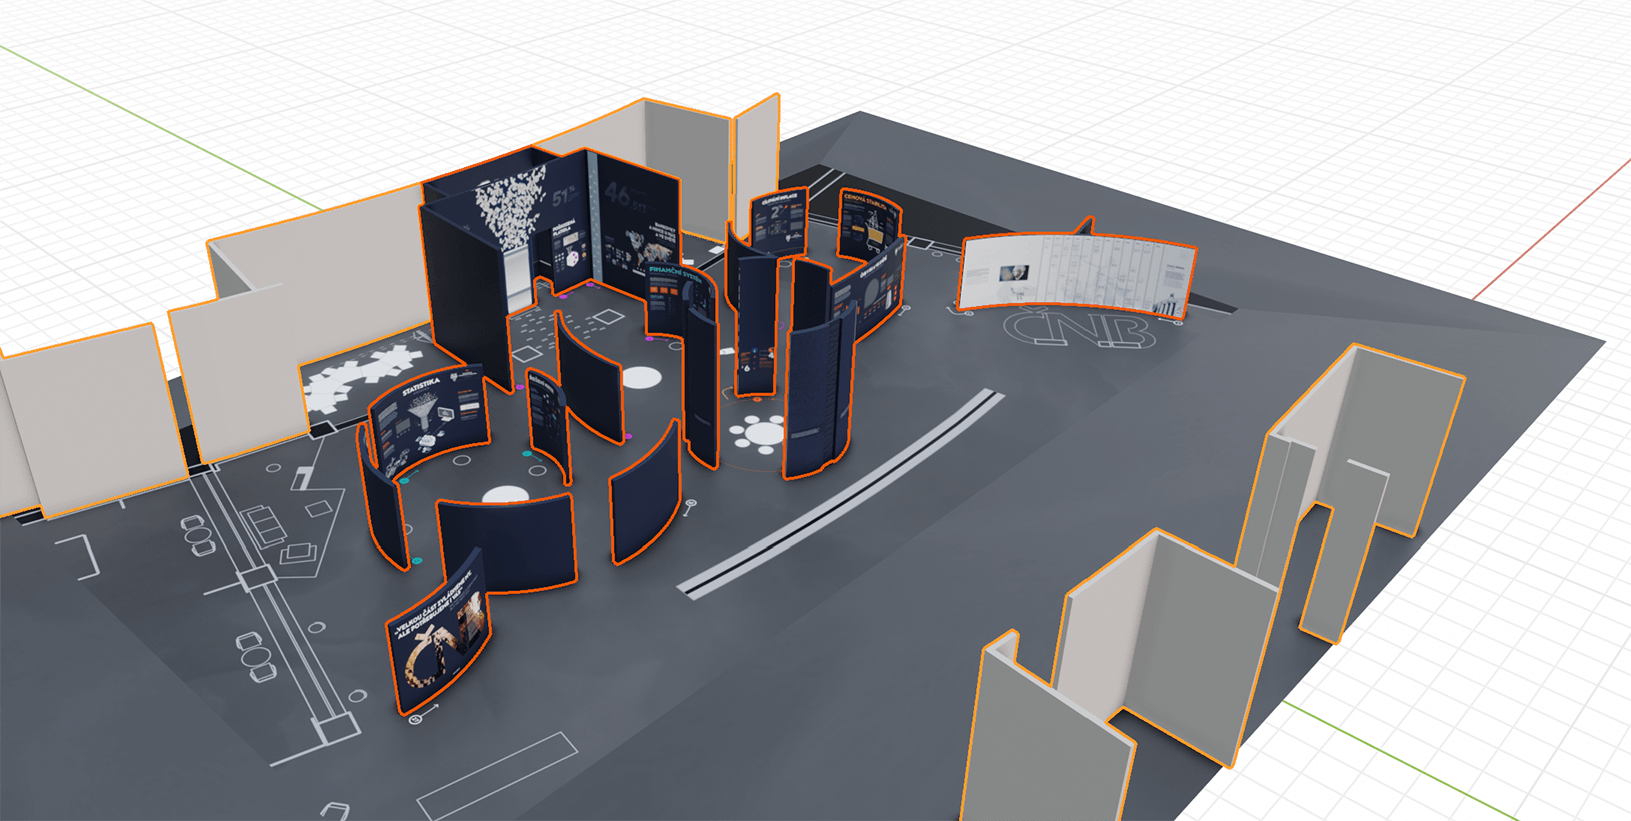
\includegraphics[width=\textwidth]{img/groupped-blender-models.png}
    \caption{Multiple meshes joined into one model.}
    \label{fig:blender-joined-objects}
\end{figure}

\begin{figure}[!ht]\centering
    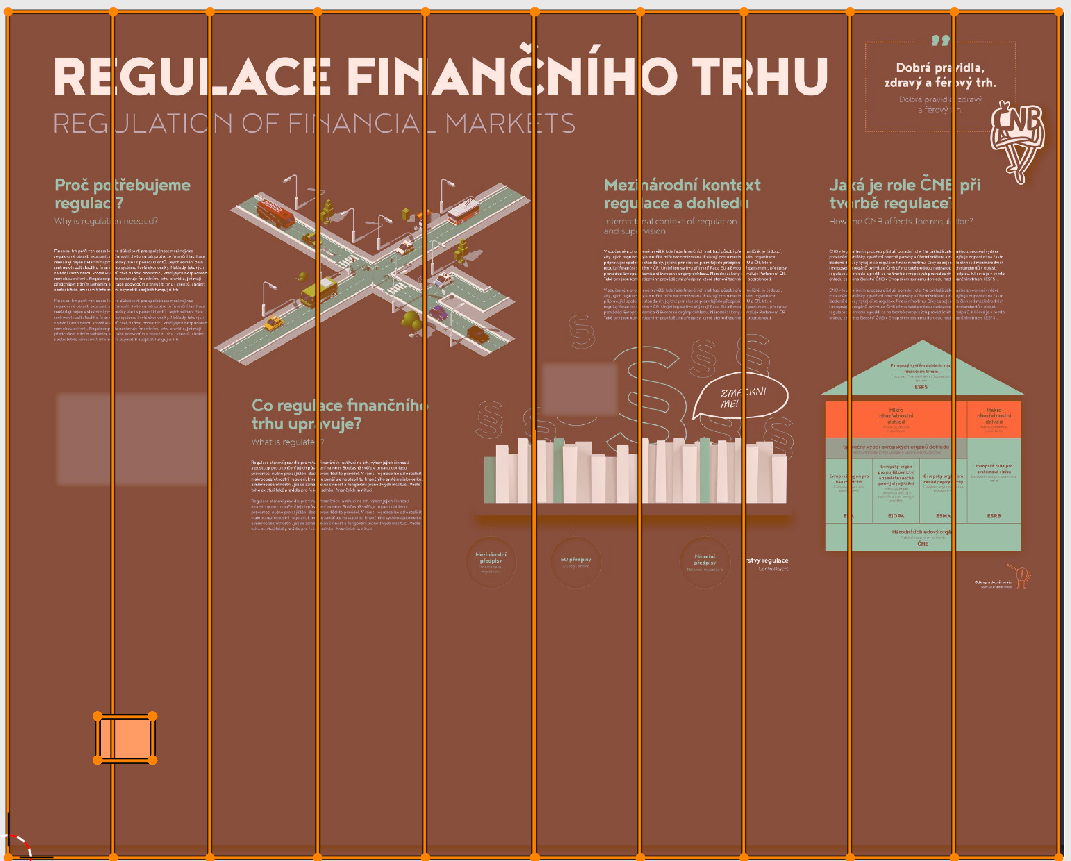
\includegraphics[width=0.55\textwidth]{img/blender-overlapping-uv.png}
    \caption{An~overlapping UV map on one information panel.}
    \label{fig:blender-overlapping-uv}
\end{figure}

\subsection{Joined objects}
The~edit mode had to select all surfaces to be separated from the~shared model and then perform the~operation shown in Figure~\ref{fig:blender-separate-selection}, separate by selection. This object then became independent in the~scene. Next, after this separation, it was worth using the~function again, but this time by material to remove loose material definitions left over from the~other meshes. This was done for all whole meshes in the~model.

Each information panel was defined by two materials. There was always a~material that displayed the~information on a~panel, but there was also a~material that used colour on its back. This colour was defined in panel 2. All the~backs of all the~panels had to be redefined to their own material to match the~original colour from panel 2.

\subsection{Overlapping UVs}
When all meshes are separate, it is important to ensure that heatmaps can be created on these objects according to the~algorithm in Section~\ref{sec:uv-unwrap-method}. It is necessary that these objects have non-overlapping UV maps defined to guarantee uniqueness for all mesh faces.

This is done in the~Object Data Properties setting of the~object. A~new map is added in the~UV Maps section and it is important to keep the~original one for the~next step. This new UV map can be defined using a~Blender feature in edit mode called Smart UV Project, which will generate the~UV map itself according to the~specified parameters. However, it is not recommended to do this without first manually defining seam edges, as, for some objects, this automatic generation could potentially yield poor results. Marking an~edge as a~seam can be seen in Figure~\ref{fig:blender-mark-seam}.

Some objects capable of being in the~Unreal project with the~plug-in have no UV maps defined or use a~basic material. These are simpler cases for which a~definition of a~new UV map is sufficient. 

\begin{figure}[!b]\centering
    \begin{subfigure}[b]{0.47\textwidth}
        \centering
        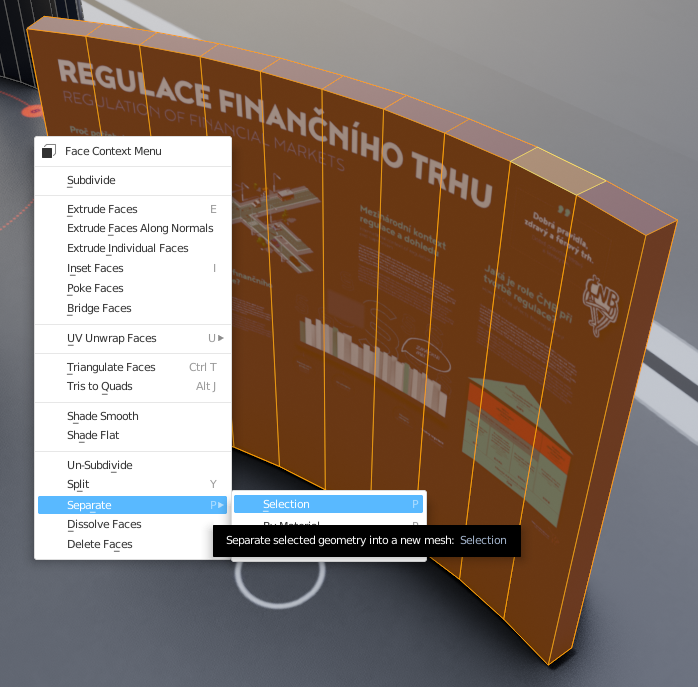
\includegraphics[width=\textwidth]{img/blender-separate-selection.png}
        \caption{Separate selection of faces into new mesh.}
        \label{fig:blender-separate-selection}
    \end{subfigure}
    \hfill
    \begin{subfigure}[b]{0.52\textwidth}
        \centering
        \includegraphics[width=\textwidth]{img/blender-mark-seam.png}
        \caption{Mark mesh edges as seam for UV unwrap.}
        \label{fig:blender-mark-seam}
    \end{subfigure}
    \caption{Blender edit mode separate selection and mark seam operations.}
\end{figure}

\pagebreak{}
\subsection{Material Baking}
This step describes the~Blender procedure to convert a~material defined for one UV map to another using texture baking. Also described in this tutorial~\cite{blender-texture-baking-tutorial}.

The~method consists of defining a~new UV map on the~same object. The~complete setup can be seen in Figure~\ref{fig:blender-bake-nodes}. Then, in the~Shader Editor, add a~new \emph{ImageTexture} material node through which a~new texture is created without an~alpha channel of square resolution. This node is connected to the~material node \emph{UV Map}, which links to the~newly created \emph{UVMapBake}. To be absolutely sure, the~original UV map can be linked to the~original texture.

\begin{figure}[!ht]\centering
    \includegraphics[width=\textwidth]{img/blender-bake-nodes.png}
    \caption{Preparation of the~information panel material nodes for baking into a~new texture.}
    \label{fig:blender-bake-nodes}
\end{figure}

To bake into UVMapBake, it is necessary to open the~Bake settings of Blender's Cycles renderer and select the~corresponding ImageTexture node. Cycles settings are in Figure~\ref{fig:blender-bake-settings}. It is enough to set the~diffuse \emph{BakeType} that will not include direct or indirect light from the~scene, only colour. The~resulting texture can be saved or embedded in the~project. The~difference between the~baked texture and the~original texture can be seen in the~Appendix~\ref{appendix:baked-textures}.

\begin{figure}[!ht]\centering
    \includegraphics[width=\textwidth]{img/blender-bake-settings.png}
    \caption{Blender cycles settings for baking simple diffuse colour onto an~ImageTexture.}
    \label{fig:blender-bake-settings}
\end{figure}

\subsection{Origin of models}
\label{sec:blender-origins}
The~original model contains many grouped objects that share a~common origin or have their origin right at the~origin of the~scene. This needs to be changed for those objects that will be exported, due to Unreal Engine's rendering pipeline, which culls in one step those objects that are not visible in the~view frustum. This happens during heatmap rendering when the~object is somewhere else than where the~Scene Capture Component is looking. Section~\ref{sec:uv-unwrap-implementation} describes how the~render Actor changes its position in the~world based on the~position of the~object being rendered. Because of this, the~mesh itself must be guaranteed to be near its origin for at least the~distance determined by the~size of the~rendered heatmap texture, which also determines the~width of the~orthographic frustum.

In Blender, it is worth setting the~length of the~units to centimetres in Scene Properties first to mimic the~unit system in Unreal. Origin can be changed in the~context of this scene in the~following style; generate a~new origin at the~centre of the~object geometry, place a~3D cursor on this new origin and set the~z-coordinate to 0 so the~cursor will sit on the~ground, and finally assign the~object's origin to this 3D cursor.

\subsection{Model export}

An~object with a~newly defined UV map, a~material that contains the~newly baked texture of the~original material, can be exported to Unreal Engine. It includes tools that allow some 3D modelling programmes to export their entire scenes at once. This is called \emph{Datasmith}. This was only available in the~past using an~unofficial Blender plug-in, which was not supported and could not be used at the~time of writing the~thesis. This route cannot be taken; the~conversion of the~whole scene is done manually.

Exporting an~object from Blender as an~\path{.fbx} file allows one to bundle its mesh, material, and texture with it. Procedural materials cannot be exported in this manner and must be baked before.

\section{Unreal project}
This section will describe how the~experiment scene was constructed by adding exported models one by one from Blender. The~entire project can be found in the~enclosed media in.

\subsection{Setting up the~scene}
The~models were inserted into the~scene inside the~logical entities represented by different Actors in the~project directory in the~Map folder, Figure~\ref{fig:cnb-scene-contents}.

\begin{figure}[!ht]\centering
    \includegraphics[width=\textwidth]{img/cnb-scene-contents.png}
    \caption{Actors containing scene objects.}
    \label{fig:cnb-scene-contents}
\end{figure}

\subsubsection*{Asset placement}
An~Fbx file can always be imported into Unreal with a~simple drag-and-drop. At most, such an~object brought StaticMesh, Material and Texture2D with it into the~project. These Assets are, respectively, divided into Geometries, Materials, and Textures directories. All imported models are in their local coordinates, guaranteed by setting up their origins according to Section~\ref{sec:blender-origins}.

For a~logical scene entity such as an~exhibit, a~single Actor was used. For this actor, several components of the~EyeTrackedStaticMeshComponent class defined in Section~\ref{sec:static-mesh-ET} were added. Those were manually placed in the~local world coordinate system of a~given Actor exactly according to the~coordinates that the~meshes would have in Blender relative to the~origin of an~exhibit. See Figure~\ref{fig:exhibit-definition}.
Each of these components has been assigned a~StaticMesh. Next, the~texture resolution and the~\emph{AcceptsHeat} boolean are set.

Not all objects from the~scene in Blender were used to keep the~experiment relatively clean. The~reason is the~recording of both heatmaps from the~eye tracker and the~virtual camera. The~simpler one has a~much larger brush radius set, so it is worth demonstrating it on objects that are large.

\begin{figure}[!ht]\centering
    \begin{subfigure}[b]{0.495\textwidth}
        \centering
        \includegraphics[width=\textwidth]{img/blender-exhibit.png}
        \caption{Panels with origin at exhibit centre in Blender.}
    \end{subfigure}
    \hfill
    \begin{subfigure}[b]{0.495\textwidth}
        \centering
        \includegraphics[width=\textwidth]{img/unreal-exhibit.png}
        \caption{Panels defined around Actor's origin in UE.}
    \end{subfigure}
    \caption{Exhibit defined as logical scene entity.}
    \label{fig:exhibit-definition}
\end{figure}

\subsubsection*{Collisions}
Each StaticMesh can be collided with using its complex collision, which is in effect just a~collision against all its faces. It is possible to define simple collisions for the~mesh in the~Static Mesh Editor in Unreal Engine to reduce the~complexity of collision calculations. For all static meshes imported from Blender, the~Convex Decomposition function in the~editor was used to generate a~simple collision volume. 

\pagebreak{}

\subsection{Pawns}
\label{sec:pawns}
In the~scene, two Pawns are defined to move around the~scene. One is used to collect data, while the~other is used only to view them. 

\subsubsection*{VRCollector}
This pawn is a~pure pawn without any movement ability. It contains the~GazeEmitter component described in Section~\ref{sec:gaze-emitter} and a~camera that is directly locked to an~absolute HMD position obtained from a~positioning system. The~problem with these coordinates is that they do not move with a~pawn in the~world; they move with it. To keep them positioned in the~same way as the~camera, it is necessary to fix the~pawn at the~origin of the~world from which it will not move. To solve this problem, the~pawn will not traverse the~scene, but the~entire scene will move around the~pawn. Specifically, in the~opposite direction to the~way the~pawn wants to move. See Figure~\ref{fig:vr-pawn-movement}. In the~whole scene, an~Actor \emph{SceneOrigin} has been created who is superior to all other Actors. 


Its main functionality, however, is that it starts an~experiment that lasts three minutes. When finished, all textures are saved in the~folder \path{C:/ProgramData/NC_ET/} and the~programme is exited, as can be seen in Figure~\ref{fig:experiment-definition}. During this experiment, data were collected using the~GazeEmitter component, Section~\ref{sec:gaze-emitter}. Figure~\ref{fig:heatmap-rendering-cycle} shows the~Tick Event of this Pawn, which always asks if the~experiment is running. If it does, it sends the~forward vector of the~Camera from its origin as a~ray classified as Camera ray type to the~\emph{Emit Ray From} function, defined in Section~\ref{sec:gaze-emitter}. It can also be seen in the~figure that the~same vector is sent for the~ray classified as Gaze. The~reason for this is discussed in Section~\ref{sec:data-collection}. The~implementation of this cycle corresponds exactly to the~activity diagram in Figure~\ref{fig:experiment-diagram} in Section~\ref{sec:plugin-functionality}.

\begin{figure}[!ht]\centering
    \includegraphics[width=\textwidth]{img/vr-pawn-movement.png}
    \caption{VRCollector movement definition.}
    \label{fig:vr-pawn-movement}
\end{figure}

\pagebreak{}

\begin{figure}[!ht]\centering
    \includegraphics[width=\textwidth]{img/experiment-definition.png}
    \caption{VRCollector set experiment start and duration.}
    \label{fig:experiment-definition}
\end{figure}

\begin{figure}[!ht]\centering
    \includegraphics[width=\textwidth]{img/heatmap-rendering-cycle.png}
    \caption{VRCollector Tick Event sending rays from virtual camera.}
    \label{fig:heatmap-rendering-cycle}
\end{figure}

\pagebreak{}

\subsubsection*{SceneObserver}

This pawn allows one to view the~scene after the~heatmaps have been measured. This is a~pawn of type Character, so it contains its own collider and basic movement functionality. Unlike the~VRCollector, this is a~pawn that traverses the~scene conventionally and bumps into objects. In Figure~\ref{fig:load-heatmaps-character} its initialisation can be seen, where it specifies its height and loads all heatmaps that are stored in the~\path{C:/ProgramData/NC_ET/} directory structure. Use the~H key to switch between heatmap visualisations. There are three different options. First, the~original material without heatmaps, then the~TrailCompare from Section~\ref{sec:trail-compare-implementation} and finally the~HeatMaterial from Section~\ref{sec:heat-material-implementation}.

\begin{figure}[!ht]\centering
    \begin{subfigure}[b]{\textwidth}
        \centering
        \includegraphics[width=0.8\textwidth]{img/initialise-character-pawn.png}
        \caption{Initialise character and load heatmaps.}
        \label{fig:load-heatmaps-character}
    \end{subfigure}
    \begin{subfigure}[b]{\textwidth}
        \centering
        \includegraphics[width=\textwidth]{img/character-traversal.png}
        \caption{Traversal character logic.}
    \end{subfigure}
    \begin{subfigure}[b]{\textwidth}
        \centering
        \includegraphics[width=0.6\textwidth]{img/toggle-heatmaps.png}
        \caption{Toggle heatmap visualisation.}
    \end{subfigure}
    \caption{SceneObserever Event Graph.}
    \label{fig:character-event-graph}
\end{figure}

\subsection{Controls}

Both Pawns use this simple control interface. All button mappings can be seen in Figure~\ref{fig:controls}.

\begin{figure}[!ht]\centering
    \includegraphics[width=\textwidth]{img/controls.png}
    \caption{Control scheme of the~unreal project with experiment.}
    \label{fig:controls}
\end{figure}

\pagebreak{}

\section{XTAL}

This section describes the~setup of the~XTAL headset within the~3D CAVE laboratory at the~Faculty of Mechanical Engineering of CTU. It also presents issues with the~current beta OpenXR runtime by Vrgineers~\cite{vrgineers-openxr-soft} and its unsuccessful troubleshooting. Note that the~lab has an~older generation of XTAL than the~current XTAL 3.

\subsection{Setup}
The~laboratory has set up several VICON tracking cameras that collectively acquire the~absolute position of defined objects in this space using small reflective spheres. Several of these spheres are attached to XTAL. The~VICON system obtains the~absolute position of these spheres and sends them as an~overall object defined as \emph{Xtal01} over the~network. In the~settings of the~VR Tool runtime, which is the~driver for the~XTAL headset~\cite{vr-tool}, the~positioning system can be set to VICON. There, it can specify the~IP address of the~system that sends these positioning data.

Regarding XTAL itself, Figure~\ref{fig:vr-tools-settings} shows the~eye runtime settings. Functions such as auto-IPD can be triggered, which is measured using ET to automatically adjust the~lens distance inside. There is also a~calibration section for the~ET. The~user must always run a~new calibration when a~programme is started. Advanced calibration is a~seven-point calibration that results in more precise measurements. 

\begin{figure}[!ht]\centering
    \includegraphics[width=0.9\textwidth]{img/runtime-eye-settings.png}
    \caption{Vrgineers VR Tool runtime eye settings.~\cite{vr-tool}}
    \label{fig:vr-tools-settings}
\end{figure}

\subsection{Troubleshooting}

The~main problem that occurred was the~instability of the~OpenXR XTAL runtime, which caused regular crashes of the~entire UEEditor during the~VR Preview in the~Unreal project. The~VR Preview sometimes lasted for a~full three minutes before crashing and sometimes did not even turn on. The~error message can be seen in Figure~\ref{fig:unreal-error-msg}.

\pagebreak{}
The~latest version of OpenXR runtime from Vrgineers~\cite{vrgineers-openxr-soft}, sent via email, was tested. The~runtime was still in beta at the~time of writing, and it was not possible to resolve this issue for Unreal Engine 4.27.

Support from Vrgineers was consulted on this issue, and they said that they are also experiencing runtime crashes of the~UEEditor for unknown reasons, but not at such frequent intervals~\cite{vrginners-email}. It has been tested to see if the~debugging tools used in UEEditor are to blame for this. Although the~crashes were not as sudden, the~project always lasted at least half a~minute; it did not solve the~problem.

While the~VR Preview was running, it was possible to calibrate the~ET and send rays out into the~scene. The~problem is that this process is rather long, and before the~participant could get to the~measuring part, the~whole programme would crash. It was tested to see if it would crash even when running the~standalone version of the~game. In this case, it was not determined whether this would solve the~problem because the~OpenXR runtime does not initialise the~XTAL headset to display the~scene inside, even though the~Start in VR option is enabled in the~project settings. The~console command ''\emph{stereo on}`` for the~Blueprint node \emph{Execute Console Command} was also tried, but nothing changed. It will run only for the~VR Preview in the~UEEditor.

The~Vrgineers support recommended migrating the~entire project to Unreal Engine 5, as it contains a~much more stable implementation of OpenXR communication. This was unsuccessful; details can be seen in the~Appendix~\ref{appendix:UE5}.

It was decided, after consultation with the~thesis supervisor, to use the~Vrgineers stable SDK plugin for Unreal Engine~\cite{vrgineers-unreal-sdk}, which includes the~original native runtime. However, this does not allow the~use of ET.

\begin{figure}[!t]\centering
    \includegraphics[width=0.95\textwidth]{img/unreal-error-msg.png}
    \caption{UEEditor crash log after OpenXR VR Preview.}
    \label{fig:unreal-error-msg}
\end{figure}

\pagebreak{}

\section{Data collecion}
\label{sec:data-collection}

Due to the~instability of the~OpenXR runtime, the~originally intended eye tracking experiment could not be performed, so it was decided that the~data would only be collected using a~forward vector camera in a~virtual scene in which the~participant would walk around using the~XTAL headset. 

The~plug-in created in this thesis, Chapter~\ref{chap:implementation}, contains raycasting functionality that can be easily used in any Unreal project. Thus, it already depends only on using a~working VR headset with ET. It has been tested on an~unstable XTAL runtime that the~feature works and sends rays into the~scene. It was not possible to use any other headset as an~alternative due to the~unavailability of other headsets and the~lack of time to incorporate the~changes into the~thesis.

The~test experiment will be carried out as originally intended, but without the~use of ET. It will collect both Gaze and Camera heatmaps, although it will only emit rays from the~forward vector of the~camera. This will serve as a~demonstration of what it would look like if working ET hardware was used.

\subsection{Test scenario}

The~test scenario used in this experiment is a~scene traversal by a~person who has not previously seen it. Each participant creates their own collection of heatmaps. These heatmaps will be used to determine which object most interested the~group of participants or where the~most textures intersected their trails.

\subsection{Measurement process}

One measurement consisted of first placing a~headset on the~participant to set their PID. Then, the~Unreal Engine project was launched with the~VRCollector pawn, defined in Section~\ref{sec:pawns}. The~XTAL in the~lab is connected to the~computer, which is used as a~backpack, to walk around the~lab. The~computational part of the~backpack had to be unplugged from the~charging dock and attached to its other part. The~backpack was put on by the~participant with the~headset. Before this, the~participant was instructed how to move around the~scene using a~game controller. They could have moved around without a~controller, but they would soon have hit a~wall in the~lab because the~exhibition is much bigger, so a~controller was necessary. The~speed of movement resembled a~fast walk. They were also informed that the~scene was an~exhibit of the~Czech National Bank. After ensuring that the~participant was ready, a~test period of three minutes was started. During this time, the~participant was free to walk around the~scene as they wished. A~participant was looking at the~scene that was with its original materials. Heatmaps were produced in the~background. At the~end of the~three minutes, all heatmaps were saved in the~\path{C:/ProgramData/NC_ET/} path and the~programme was stopped.

Videos of the~measurements were recorded. Participants 4 and 8 were chosen to demonstrate the~experiment. Their recorded session is in the~enclosed media in the~\path{video} folder. All heatmaps from all participants are compressed in the~\path{experiment/data/ParticipantData.zip} file.


\section{Resultant data}

A~total of 12 measurements were made, so 12 different heatmap collections were produced. These data were grouped into the~DATA folder and each measurement was in the~folder of a~numbered participant. Each participant contains a~Camera and Gaze folder, due to the~two different types of heatmap. The~Python merger script from Section~\ref{sec:python} was put in the~same folder, which merged these participants into folder \path{ResultantData}. The~same folder is in the~enclosed media in the~\path{data} folder.

There are several information panels in the~exhibition scene. The~resultant data showed that they were the~majority target of interest. It is possible to turn on the~Unreal Project and view the~data by running the~scene with the~SceneObserver pawn. The~data folder structure, along with the~Gaze and Camera folders, should be put in the~\path{C:/ProgramData/NC_ET/} folder to view them. The~scene traversal with the~resultant data can also be viewed in \path{video/05-resultant-data-showcase.mp4}.

From the~resultant data, the~four panels that showed the~highest trail densities were selected.

\subsubsection*{Panel11}
In Figure~\ref{fig:Panel11-object-heatmaps.} it is possible to see the~difference in the~textures collected of the~\emph{Panel11} scene object.
Panel11 has the~highest intensity of its trails of all the~objects in the~scene, as shown in Figure~\ref{fig:panel11-heatmap}. The~density, on the~other hand, is not large and it can be seen that large brushes were used to produce it. This means that the~participants were looking at the~object from a~longer distance. Particularly at the~beginning of the~scene while looking around to the~left or right, this is one of the~first objects visible in the~scene. 
Five participants did not even see the~object. Only three examined it. Participant 7 is an~outlier who looked at the~object for much longer and contributed greatly to the~result. 

\subsubsection*{Panel14}
Panel14 in Figure~\ref{fig:Panel14-object-heatmaps} shows the~different variations of the~heatmaps collected from the~participants and immediately Figure~\ref{fig:Panel14-resultant-heatmaps.} shows the~resulting texture and its comparison with the~original material. Only three participants have not seen this object. Unlike Panel11, this time the~object was not only viewed from a~distance, but also seen from up close by five participants. Since it has much higher density of different twisting trails.

\subsubsection*{Panel17}
Like the~previous cases, the~results are illustrated in Figures~\ref{fig:Panel17-object-heatmaps.}~and~\ref{fig:Panel17-resultant-heatmaps.}. This is the~same case as the~Panel14. It was examined up close. Compared to the~rest, it shows in its trails that more participants noticed the~mascot of the~Czech National Bank. It is the~only object that has this part of its panel highlighted together with Panel1.

\subsubsection*{Panel2}
The~panel with the~highest trail density on its surface was Panel2, which has the~advantage of being two-sided; it has graphics on both of its sides. It is located right among the~first objects in the~whole scene, next to the~large CNB logo. Figures~\ref{fig:Panel2-object-heatmaps.} and \ref{fig:Panel2-resultant-heatmaps.}.

\newpage{}

\begin{figure}[!ht]\centering
    \begin{subfigure}[b]{0.24\textwidth}
        \centering
        \includegraphics[width=\textwidth]{img/data/Panel11/single/1.png}
        \caption{Participant 1.}
    \end{subfigure}
    \hfill
    \begin{subfigure}[b]{0.24\textwidth}
        \centering
        \includegraphics[width=\textwidth]{img/data/Panel11/single/2.png}
        \caption{Participant 2.}
    \end{subfigure}
    \hfill
    \begin{subfigure}[b]{0.24\textwidth}
        \centering
        \includegraphics[width=\textwidth]{img/data/Panel11/single/3.png}
        \caption{Participant 3.}
    \end{subfigure}
    \hfill
    \begin{subfigure}[b]{0.24\textwidth}
        \centering
        \includegraphics[width=\textwidth]{img/data/Panel11/single/4.png}
        \caption{Participant 4.}
    \end{subfigure}
    \hfill
    \begin{subfigure}[b]{0.24\textwidth}
        \centering
        \includegraphics[width=\textwidth]{img/data/Panel11/single/5.png}
        \caption{Participant 5.}
    \end{subfigure}
    \hfill    
    \begin{subfigure}[b]{0.24\textwidth}
        \centering
        \includegraphics[width=\textwidth]{img/data/Panel11/single/6.png}
        \caption{Participant 6.}
    \end{subfigure}
    \hfill    
    \begin{subfigure}[b]{0.24\textwidth}
        \centering
        \includegraphics[width=\textwidth]{img/data/Panel11/single/7.png}
        \caption{Participant 7.}
    \end{subfigure}
    \hfill    
    \begin{subfigure}[b]{0.24\textwidth}
        \centering
        \includegraphics[width=\textwidth]{img/data/Panel11/single/8.png}
        \caption{Participant 8.}
    \end{subfigure}
    \hfill    
    \begin{subfigure}[b]{0.24\textwidth}
        \centering
        \includegraphics[width=\textwidth]{img/data/Panel11/single/9.png}
        \caption{Participant 9.}
    \end{subfigure}
    \hfill    
    \begin{subfigure}[b]{0.24\textwidth}
        \centering
        \includegraphics[width=\textwidth]{img/data/Panel11/single/10.png}
        \caption{Participant 10.}
    \end{subfigure}
    \hfill    
    \begin{subfigure}[b]{0.24\textwidth}
        \centering
        \includegraphics[width=\textwidth]{img/data/Panel11/single/11.png}
        \caption{Participant 11.}
    \end{subfigure}
    \hfill    
    \begin{subfigure}[b]{0.24\textwidth}
        \centering
        \includegraphics[width=\textwidth]{img/data/Panel11/single/12.png}
        \caption{Participant 12.}
    \end{subfigure}
    \caption{Heatmap texture variants of Panel11 object.}
    \label{fig:Panel11-object-heatmaps.}
\end{figure}


\begin{figure}[!ht]\centering
    \begin{subfigure}[b]{0.31\textwidth}
        \centering
        \includegraphics[width=\textwidth]{img/data/Panel11/resultant/Result.png}
        \caption{Result gaze heatmap texture.}
    \end{subfigure}
    \hfill
    \begin{subfigure}[b]{0.335\textwidth}
        \centering
        \includegraphics[width=\textwidth]{img/data/Panel11/resultant/heatmap.png}
        \caption{Result gaze heatmap on object.}
        \label{fig:panel11-heatmap}
    \end{subfigure}
    \hfill
    \begin{subfigure}[b]{0.33\textwidth}
        \centering
        \includegraphics[width=\textwidth]{img/data/Panel11/resultant/original.png}
        \caption{Panel11 original material.}
    \end{subfigure}
    \caption{Resultant heatmap of Panel11.}
    \label{fig:Panel11-resultant-heatmaps.}
\end{figure}


\begin{figure}[!ht]\centering
    \begin{subfigure}[b]{0.24\textwidth}
        \centering
        \includegraphics[width=\textwidth]{img/data/Panel14/single/1.png}
        \caption{Participant 1.}
    \end{subfigure}
    \hfill
    \begin{subfigure}[b]{0.24\textwidth}
        \centering
        \includegraphics[width=\textwidth]{img/data/Panel14/single/2.png}
        \caption{Participant 2.}
    \end{subfigure}
    \hfill
    \begin{subfigure}[b]{0.24\textwidth}
        \centering
        \includegraphics[width=\textwidth]{img/data/Panel14/single/3.png}
        \caption{Participant 3.}
    \end{subfigure}
    \hfill
    \begin{subfigure}[b]{0.24\textwidth}
        \centering
        \includegraphics[width=\textwidth]{img/data/Panel14/single/4.png}
        \caption{Participant 4.}
    \end{subfigure}
    \hfill
    \begin{subfigure}[b]{0.24\textwidth}
        \centering
        \includegraphics[width=\textwidth]{img/data/Panel14/single/5.png}
        \caption{Participant 5.}
    \end{subfigure}
    \hfill    
    \begin{subfigure}[b]{0.24\textwidth}
        \centering
        \includegraphics[width=\textwidth]{img/data/Panel14/single/6.png}
        \caption{Participant 6.}
    \end{subfigure}
    \hfill    
    \begin{subfigure}[b]{0.24\textwidth}
        \centering
        \includegraphics[width=\textwidth]{img/data/Panel14/single/7.png}
        \caption{Participant 7.}
    \end{subfigure}
    \hfill    
    \begin{subfigure}[b]{0.24\textwidth}
        \centering
        \includegraphics[width=\textwidth]{img/data/Panel14/single/8.png}
        \caption{Participant 8.}
    \end{subfigure}
    \hfill    
    \begin{subfigure}[b]{0.24\textwidth}
        \centering
        \includegraphics[width=\textwidth]{img/data/Panel14/single/9.png}
        \caption{Participant 9.}
    \end{subfigure}
    \hfill    
    \begin{subfigure}[b]{0.24\textwidth}
        \centering
        \includegraphics[width=\textwidth]{img/data/Panel14/single/10.png}
        \caption{Participant 10.}
    \end{subfigure}
    \hfill    
    \begin{subfigure}[b]{0.24\textwidth}
        \centering
        \includegraphics[width=\textwidth]{img/data/Panel14/single/11.png}
        \caption{Participant 11.}
    \end{subfigure}
    \hfill    
    \begin{subfigure}[b]{0.24\textwidth}
        \centering
        \includegraphics[width=\textwidth]{img/data/Panel14/single/12.png}
        \caption{Participant 12.}
    \end{subfigure}
    \caption{Heatmap texture variants of Panel14 object.}
    \label{fig:Panel14-object-heatmaps}
\end{figure}


\begin{figure}[!ht]\centering
    \begin{subfigure}[b]{0.32\textwidth}
        \centering
        \includegraphics[width=\textwidth]{img/data/Panel14/resultant/Result.png}
        \caption{Result gaze heatmap texture.}
    \end{subfigure}
    \hfill
    \begin{subfigure}[b]{0.325\textwidth}
        \centering
        \includegraphics[width=\textwidth]{img/data/Panel14/resultant/heatmap.png}
        \caption{Result gaze heatmap on object.}
    \end{subfigure}
    \hfill
    \begin{subfigure}[b]{0.32\textwidth}
        \centering
        \includegraphics[width=\textwidth]{img/data/Panel14/resultant/original.png}
        \caption{Panel14 original material.}
    \end{subfigure}
    \caption{Resultant heatmap of Panel14.}
    \label{fig:Panel14-resultant-heatmaps.}
\end{figure}



\begin{figure}[!ht]\centering
    \begin{subfigure}[b]{0.24\textwidth}
        \centering
        \includegraphics[width=\textwidth]{img/data/Panel17/single/1.png}
        \caption{Participant 1.}
    \end{subfigure}
    \hfill
    \begin{subfigure}[b]{0.24\textwidth}
        \centering
        \includegraphics[width=\textwidth]{img/data/Panel17/single/2.png}
        \caption{Participant 2.}
    \end{subfigure}
    \hfill
    \begin{subfigure}[b]{0.24\textwidth}
        \centering
        \includegraphics[width=\textwidth]{img/data/Panel17/single/3.png}
        \caption{Participant 3.}
    \end{subfigure}
    \hfill
    \begin{subfigure}[b]{0.24\textwidth}
        \centering
        \includegraphics[width=\textwidth]{img/data/Panel17/single/4.png}
        \caption{Participant 4.}
    \end{subfigure}
    \hfill
    \begin{subfigure}[b]{0.24\textwidth}
        \centering
        \includegraphics[width=\textwidth]{img/data/Panel17/single/5.png}
        \caption{Participant 5.}
    \end{subfigure}
    \hfill    
    \begin{subfigure}[b]{0.24\textwidth}
        \centering
        \includegraphics[width=\textwidth]{img/data/Panel17/single/6.png}
        \caption{Participant 6.}
    \end{subfigure}
    \hfill    
    \begin{subfigure}[b]{0.24\textwidth}
        \centering
        \includegraphics[width=\textwidth]{img/data/Panel17/single/7.png}
        \caption{Participant 7.}
    \end{subfigure}
    \hfill    
    \begin{subfigure}[b]{0.24\textwidth}
        \centering
        \includegraphics[width=\textwidth]{img/data/Panel17/single/8.png}
        \caption{Participant 8.}
    \end{subfigure}
    \hfill    
    \begin{subfigure}[b]{0.24\textwidth}
        \centering
        \includegraphics[width=\textwidth]{img/data/Panel17/single/9.png}
        \caption{Participant 9.}
    \end{subfigure}
    \hfill    
    \begin{subfigure}[b]{0.24\textwidth}
        \centering
        \includegraphics[width=\textwidth]{img/data/Panel17/single/10.png}
        \caption{Participant 10.}
    \end{subfigure}
    \hfill    
    \begin{subfigure}[b]{0.24\textwidth}
        \centering
        \includegraphics[width=\textwidth]{img/data/Panel17/single/11.png}
        \caption{Participant 11.}
    \end{subfigure}
    \hfill    
    \begin{subfigure}[b]{0.24\textwidth}
        \centering
        \includegraphics[width=\textwidth]{img/data/Panel17/single/12.png}
        \caption{Participant 12.}
    \end{subfigure}
    \caption{Heatmap texture variants of Panel17 object.}
    \label{fig:Panel17-object-heatmaps.}
\end{figure}


\begin{figure}[!ht]\centering
    \begin{subfigure}[b]{0.31\textwidth}
        \centering
        \includegraphics[width=\textwidth]{img/data/Panel17/resultant/Result.png}
        \caption{Result gaze heatmap texture.}
    \end{subfigure}
    \hfill
    \begin{subfigure}[b]{0.335\textwidth}
        \centering
        \includegraphics[width=\textwidth]{img/data/Panel17/resultant/heatmap.png}
        \caption{Result gaze heatmap on object.}
    \end{subfigure}
    \hfill
    \begin{subfigure}[b]{0.33\textwidth}
        \centering
        \includegraphics[width=\textwidth]{img/data/Panel17/resultant/original.png}
        \caption{Panel17 original material.}
    \end{subfigure}
    \caption{Resultant heatmap of Panel17.}
    \label{fig:Panel17-resultant-heatmaps.}
\end{figure}

\begin{figure}[!ht]\centering
    \begin{subfigure}[b]{0.24\textwidth}
        \centering
        \includegraphics[width=\textwidth]{img/data/Panel2/single/1.png}
        \caption{Participant 1.}
    \end{subfigure}
    \hfill
    \begin{subfigure}[b]{0.24\textwidth}
        \centering
        \includegraphics[width=\textwidth]{img/data/Panel2/single/2.png}
        \caption{Participant 2.}
    \end{subfigure}
    \hfill
    \begin{subfigure}[b]{0.24\textwidth}
        \centering
        \includegraphics[width=\textwidth]{img/data/Panel2/single/3.png}
        \caption{Participant 3.}
    \end{subfigure}
    \hfill
    \begin{subfigure}[b]{0.24\textwidth}
        \centering
        \includegraphics[width=\textwidth]{img/data/Panel2/single/4.png}
        \caption{Participant 4.}
    \end{subfigure}
    \hfill
    \begin{subfigure}[b]{0.24\textwidth}
        \centering
        \includegraphics[width=\textwidth]{img/data/Panel2/single/5.png}
        \caption{Participant 5.}
    \end{subfigure}
    \hfill    
    \begin{subfigure}[b]{0.24\textwidth}
        \centering
        \includegraphics[width=\textwidth]{img/data/Panel2/single/6.png}
        \caption{Participant 6.}
    \end{subfigure}
    \hfill    
    \begin{subfigure}[b]{0.24\textwidth}
        \centering
        \includegraphics[width=\textwidth]{img/data/Panel2/single/7.png}
        \caption{Participant 7.}
    \end{subfigure}
    \hfill    
    \begin{subfigure}[b]{0.24\textwidth}
        \centering
        \includegraphics[width=\textwidth]{img/data/Panel2/single/8.png}
        \caption{Participant 8.}
    \end{subfigure}
    \hfill    
    \begin{subfigure}[b]{0.24\textwidth}
        \centering
        \includegraphics[width=\textwidth]{img/data/Panel2/single/9.png}
        \caption{Participant 9.}
    \end{subfigure}
    \hfill    
    \begin{subfigure}[b]{0.24\textwidth}
        \centering
        \includegraphics[width=\textwidth]{img/data/Panel2/single/10.png}
        \caption{Participant 10.}
    \end{subfigure}
    \hfill    
    \begin{subfigure}[b]{0.24\textwidth}
        \centering
        \includegraphics[width=\textwidth]{img/data/Panel2/single/11.png}
        \caption{Participant 11.}
    \end{subfigure}
    \hfill    
    \begin{subfigure}[b]{0.24\textwidth}
        \centering
        \includegraphics[width=\textwidth]{img/data/Panel2/single/12.png}
        \caption{Participant 12.}
    \end{subfigure}
    \caption{Heatmap texture variants of Panel2 object.}
    \label{fig:Panel2-object-heatmaps.}
\end{figure}


\begin{figure}[!ht]\centering
    \begin{subfigure}[b]{0.32\textwidth}
        \centering
        \includegraphics[width=\textwidth]{img/data/Panel2/resultant/Result.png}
        \caption{Result gaze heatmap texture.}
    \end{subfigure}
    \hfill
    \begin{subfigure}[b]{0.32\textwidth}
        \centering
        \includegraphics[width=\textwidth]{img/data/Panel2/resultant/heatmap.png}
        \caption{Result gaze heatmap on object.}
    \end{subfigure}
    \hfill
    \begin{subfigure}[b]{0.305\textwidth}
        \centering
        \includegraphics[width=\textwidth]{img/data/Panel2/resultant/original.png}
        \caption{Panel2 original material.}
    \end{subfigure}
    \caption{Resultant heatmap of Panel2.}
    \label{fig:Panel2-resultant-heatmaps.}
\end{figure}



\chapter{Conclusion}

The~main goal of this thesis was to develop a~prototype application inside a~modern game engine that collects and visualises gaze data and use it to build an~experiment that collects data from multiple participants inside a~3D virtual scene. 

An~analysis of existing hardware and software solutions that use eye tracking was performed. Based on this analysis, it was decided that the~prototype application would be designed as a~plug-in for Unreal Engine 4. The~plugin extends the~functionality of the~engine with the~ability to create heatmaps in real-time using raycasting, which was designed to be independent of any specific ET hardware. The~only thing the~plug-in needs is a~gaze origin and direction in world coordinates. The~plug-in allows two types of heatmap to be captured at once. One that collects gaze data and one that collects forward vectors of a~virtual camera. It is possible to visualise their mutual appearance. 

An~Unreal Engine scene was created from a~prototype 3D model of the~Czech National Bank Visitor Centre in Blender. It was originally intended to use the~XTAL headset to collect gaze data, but due to the~instability of its OpenXR runtime in Unreal Engine this could not be accomplished. Several unsuccessful attempts were made to fix the~bug. Among them was the~migration of the~experiment project to the~new Unreal Engine 5. Data collection from multiple participants was done with XTAL, but only using forward vectors of the~virtual camera.

Heatmaps were collected from 12 different participants. These data were processed into resultant data that visualised the~collective visual attention of this group of participants. From this, it was evaluated which objects in the~scene were noticed the~most and why. 


\section*{Future Work}

This thesis offers a~working prototype of a~plug-in for UE4 that collects and visualises gaze data using heatmaps that can be used to produce more complicated experiments exploring the~behaviour of a~much larger group of people than was used in this thesis. It is possible to try any other VR headset with ET. There is plenty of room for improvement. One of the~main ideas that had not been done, because it was not even possible to test, is the~classification of gaze data into saccades and fixations. Synchronise with the~maximum output that the~eye tracker offers and perform these classifications faster than each Tick. This could be used to create a~scanpath or to store fixation metrics per region of interest in real time. This would allow for the~implementation of other visualisation and data collection methods.

One way to extend it would be to implement an~objective-based system similar to the~one described in the~analysis of Cognitive3D's software that would attach gaze events to objects that will get triggered when it is gazed at. 
\appendix\appendixinit % do not remove these two commands

\chapter{Unreal Engine 5 migration}
\label{appendix:UE5}

The plug-in that was created in this work was simple to migrate to Unreal Engine 5. All that had to be done was to download the engine, create a new project, and then copy the previous \path{.uasset} files of the Blueprints and Materials in UE4 into the project. The entire experiment scene was copied into UE5 exactly the same way.

\bigskip{}
Immediately it was tested if the entire UEEditor would crash after running it with the XTAL headset, for normal scene traversal. This time it did not crash even once. However, another problem occurred during ET calibration in XTAL. Not a single calibration succeeded; all of them caused the UEEditor to crash while the OpenXR Eye Tracking plug-in was enabled. 

\bigskip{}
This was not even consulted with support, as another issue was discovered that was not related to the headset. The technique of drawing heatmaps using a 3D brush stopped working. In the latest version of UE5, the Additive Composite mode of the Scene Capture Component does not work properly. In the official Unreal Engine forums, several users reported the same problem during UE5 beta testing~\cite{unreal-forum}. The additive and composite mode of the Scene Capture Component behave the same as the overwrite mode. This bug was not fixed before submitting this thesis. Causes the heatmap texture to always be overwritten with a new brush according to the collision. This method could be used when the Epic Games team fixes the bug.

\bigskip{}
It was not possible to use Unreal Engine 5 to collect ET data with the prototype plug-in. The~migrated UE5 version of the experiment scene can be found in the enclosed media in the~\path{experiment/project/CNB_NC_ET_UE5.zip} file.

\chapter{ET Component DMI initialisation}
\label{appendix:ETcomponent}

\begin{figure}[!ht]
    \centering
    \includegraphics[width=\textwidth]{img/appendix/ETcomponent-DMI.png}
\end{figure}

\chapter{Baked texture difference}
\label{appendix:baked-textures}

\begin{figure}[!b]\centering
    \begin{subfigure}[b]{0.5\textwidth}
        \centering
        \includegraphics[width=\textwidth]{img/appendix/panel-bake-uv.png}
    \end{subfigure}
    \hfill
    \begin{subfigure}[b]{0.6\textwidth}
        \centering
        \includegraphics[width=\textwidth]{img/appendix/panel-bake-original.png}
    \end{subfigure}
\end{figure} % include `appendix.tex' from `text/' subdirectory

\backmatter % do not remove this command

\printbibliography % print out the~BibLaTeX-generated bibliography list

\chapter{Contents of the enclosed media}

The contents are also available on faculty GitLab:

\url{https://gitlab.fit.cvut.cz/kvasnric/bp_kvasnric}.
\bigskip{}

	\dirtree{%
		.1 experiment\DTcomment{the directory with Unreal Engine project of the experiment}.
		.2 data\DTcomment{the directory with collected heatmap textures}.
		.3 Participantdata.zip\DTcomment{compressed zip archive of heatmap textures from participants}.
		.3 ResultantData.zip\DTcomment{compressed zip archive of resultant heatmap textures}.
		.2 model\DTcomment{the directory with Blender projects}.
		.3 CNB-NC-original.blend\DTcomment{Visitor Centre CNB 3D original model}.
		.3 CNB-NC-modified.blend\DTcomment{Visitor Centre CNB 3D model ready for export to UE}.
		.2 project\DTcomment{the directory with Visitor Centre CNB Unreal Engine projects}.
		.3 CNB\_NC\_ET.zip\DTcomment{zip archive with project in Unreal Engine 4}.
		.3 CNB\_NC\_ET\_UE5.zip\DTcomment{zip archive with project in Unreal Engine 5}.
		.1 src\DTcomment{the directory of source codes}.
		.2 plug-in\DTcomment{the Unreal Engine prototype plug-in source}.
		.2 thesis\DTcomment{the directory of \LaTeX{} source codes of the thesis}.
		.2 python\DTcomment{the directory with Python source codes}.
		.3 merger.py\DTcomment{the EXR image merger script}.
		.1 text\DTcomment{the thesis text directory}.
		.2 thesis.pdf\DTcomment{the thesis text in PDF format}.
		.1 video\DTcomment{the directory with video demonstrations}.
		.2 01-basic-painting-method.mp4\DTcomment{H265 videofile}.
		.2 02-3D-brush-problem.mp4\DTcomment{H265 videofile}.
		.2 03-simple-collision-only.mp4\DTcomment{H265 videofile}.
		.2 04-creating-heatmaps.mp4\DTcomment{H265 videofile}.
		.2 05-resultant-data-showcase.mp4\DTcomment{H265 videofile}.
		.2 06-participant4.mkv\DTcomment{H265 videofile}.
		.2 07-participant8.mkv\DTcomment{H265 videofile}.
	}
 % include `medium.tex' from `text/' subdirectory

\end{document}
